% Options for packages loaded elsewhere
\PassOptionsToPackage{unicode}{hyperref}
\PassOptionsToPackage{hyphens}{url}
%
\documentclass[
]{book}
\usepackage{amsmath,amssymb}
\usepackage{iftex}
\ifPDFTeX
  \usepackage[T1]{fontenc}
  \usepackage[utf8]{inputenc}
  \usepackage{textcomp} % provide euro and other symbols
\else % if luatex or xetex
  \usepackage{unicode-math} % this also loads fontspec
  \defaultfontfeatures{Scale=MatchLowercase}
  \defaultfontfeatures[\rmfamily]{Ligatures=TeX,Scale=1}
\fi
\usepackage{lmodern}
\ifPDFTeX\else
  % xetex/luatex font selection
\fi
% Use upquote if available, for straight quotes in verbatim environments
\IfFileExists{upquote.sty}{\usepackage{upquote}}{}
\IfFileExists{microtype.sty}{% use microtype if available
  \usepackage[]{microtype}
  \UseMicrotypeSet[protrusion]{basicmath} % disable protrusion for tt fonts
}{}
\makeatletter
\@ifundefined{KOMAClassName}{% if non-KOMA class
  \IfFileExists{parskip.sty}{%
    \usepackage{parskip}
  }{% else
    \setlength{\parindent}{0pt}
    \setlength{\parskip}{6pt plus 2pt minus 1pt}}
}{% if KOMA class
  \KOMAoptions{parskip=half}}
\makeatother
\usepackage{xcolor}
\usepackage{color}
\usepackage{fancyvrb}
\newcommand{\VerbBar}{|}
\newcommand{\VERB}{\Verb[commandchars=\\\{\}]}
\DefineVerbatimEnvironment{Highlighting}{Verbatim}{commandchars=\\\{\}}
% Add ',fontsize=\small' for more characters per line
\usepackage{framed}
\definecolor{shadecolor}{RGB}{248,248,248}
\newenvironment{Shaded}{\begin{snugshade}}{\end{snugshade}}
\newcommand{\AlertTok}[1]{\textcolor[rgb]{0.94,0.16,0.16}{#1}}
\newcommand{\AnnotationTok}[1]{\textcolor[rgb]{0.56,0.35,0.01}{\textbf{\textit{#1}}}}
\newcommand{\AttributeTok}[1]{\textcolor[rgb]{0.13,0.29,0.53}{#1}}
\newcommand{\BaseNTok}[1]{\textcolor[rgb]{0.00,0.00,0.81}{#1}}
\newcommand{\BuiltInTok}[1]{#1}
\newcommand{\CharTok}[1]{\textcolor[rgb]{0.31,0.60,0.02}{#1}}
\newcommand{\CommentTok}[1]{\textcolor[rgb]{0.56,0.35,0.01}{\textit{#1}}}
\newcommand{\CommentVarTok}[1]{\textcolor[rgb]{0.56,0.35,0.01}{\textbf{\textit{#1}}}}
\newcommand{\ConstantTok}[1]{\textcolor[rgb]{0.56,0.35,0.01}{#1}}
\newcommand{\ControlFlowTok}[1]{\textcolor[rgb]{0.13,0.29,0.53}{\textbf{#1}}}
\newcommand{\DataTypeTok}[1]{\textcolor[rgb]{0.13,0.29,0.53}{#1}}
\newcommand{\DecValTok}[1]{\textcolor[rgb]{0.00,0.00,0.81}{#1}}
\newcommand{\DocumentationTok}[1]{\textcolor[rgb]{0.56,0.35,0.01}{\textbf{\textit{#1}}}}
\newcommand{\ErrorTok}[1]{\textcolor[rgb]{0.64,0.00,0.00}{\textbf{#1}}}
\newcommand{\ExtensionTok}[1]{#1}
\newcommand{\FloatTok}[1]{\textcolor[rgb]{0.00,0.00,0.81}{#1}}
\newcommand{\FunctionTok}[1]{\textcolor[rgb]{0.13,0.29,0.53}{\textbf{#1}}}
\newcommand{\ImportTok}[1]{#1}
\newcommand{\InformationTok}[1]{\textcolor[rgb]{0.56,0.35,0.01}{\textbf{\textit{#1}}}}
\newcommand{\KeywordTok}[1]{\textcolor[rgb]{0.13,0.29,0.53}{\textbf{#1}}}
\newcommand{\NormalTok}[1]{#1}
\newcommand{\OperatorTok}[1]{\textcolor[rgb]{0.81,0.36,0.00}{\textbf{#1}}}
\newcommand{\OtherTok}[1]{\textcolor[rgb]{0.56,0.35,0.01}{#1}}
\newcommand{\PreprocessorTok}[1]{\textcolor[rgb]{0.56,0.35,0.01}{\textit{#1}}}
\newcommand{\RegionMarkerTok}[1]{#1}
\newcommand{\SpecialCharTok}[1]{\textcolor[rgb]{0.81,0.36,0.00}{\textbf{#1}}}
\newcommand{\SpecialStringTok}[1]{\textcolor[rgb]{0.31,0.60,0.02}{#1}}
\newcommand{\StringTok}[1]{\textcolor[rgb]{0.31,0.60,0.02}{#1}}
\newcommand{\VariableTok}[1]{\textcolor[rgb]{0.00,0.00,0.00}{#1}}
\newcommand{\VerbatimStringTok}[1]{\textcolor[rgb]{0.31,0.60,0.02}{#1}}
\newcommand{\WarningTok}[1]{\textcolor[rgb]{0.56,0.35,0.01}{\textbf{\textit{#1}}}}
\usepackage{longtable,booktabs,array}
\usepackage{calc} % for calculating minipage widths
% Correct order of tables after \paragraph or \subparagraph
\usepackage{etoolbox}
\makeatletter
\patchcmd\longtable{\par}{\if@noskipsec\mbox{}\fi\par}{}{}
\makeatother
% Allow footnotes in longtable head/foot
\IfFileExists{footnotehyper.sty}{\usepackage{footnotehyper}}{\usepackage{footnote}}
\makesavenoteenv{longtable}
\usepackage{graphicx}
\makeatletter
\def\maxwidth{\ifdim\Gin@nat@width>\linewidth\linewidth\else\Gin@nat@width\fi}
\def\maxheight{\ifdim\Gin@nat@height>\textheight\textheight\else\Gin@nat@height\fi}
\makeatother
% Scale images if necessary, so that they will not overflow the page
% margins by default, and it is still possible to overwrite the defaults
% using explicit options in \includegraphics[width, height, ...]{}
\setkeys{Gin}{width=\maxwidth,height=\maxheight,keepaspectratio}
% Set default figure placement to htbp
\makeatletter
\def\fps@figure{htbp}
\makeatother
\ifLuaTeX
  \usepackage{luacolor}
  \usepackage[soul]{lua-ul}
\else
  \usepackage{soul}
\fi
\setlength{\emergencystretch}{3em} % prevent overfull lines
\providecommand{\tightlist}{%
  \setlength{\itemsep}{0pt}\setlength{\parskip}{0pt}}
\setcounter{secnumdepth}{5}
\usepackage{booktabs}
\ifLuaTeX
  \usepackage{selnolig}  % disable illegal ligatures
\fi
\usepackage[]{natbib}
\bibliographystyle{plainnat}
\usepackage{bookmark}
\IfFileExists{xurl.sty}{\usepackage{xurl}}{} % add URL line breaks if available
\urlstyle{same}
\hypersetup{
  pdftitle={ShiNyP: User Guide},
  hidelinks,
  pdfcreator={LaTeX via pandoc}}

\title{ShiNyP: User Guide}
\author{true}
\date{Oct 2024}

\begin{document}
\maketitle

{
\setcounter{tocdepth}{1}
\tableofcontents
}
\chapter{Quickstart}\label{quickstart}

\textbf{Step 1: Pre-install Required Package}

\begin{Shaded}
\begin{Highlighting}[]
\FunctionTok{install.packages}\NormalTok{(}\StringTok{"BiocManager"}\NormalTok{)}
\NormalTok{BiocManager}\SpecialCharTok{::}\FunctionTok{install}\NormalTok{(}\AttributeTok{version =} \StringTok{"3.19"}\NormalTok{)}
\NormalTok{BiocManager}\SpecialCharTok{::}\FunctionTok{install}\NormalTok{(}\StringTok{"qvalue"}\NormalTok{)}
\end{Highlighting}
\end{Shaded}

\textbf{Step 2: Install the {\emph{ShiNyP}}} \textbf{Package from GitHub}

\begin{Shaded}
\begin{Highlighting}[]
\FunctionTok{install.packages}\NormalTok{(}\StringTok{"remotes"}\NormalTok{) }
\NormalTok{remotes}\SpecialCharTok{::}\FunctionTok{install\_github}\NormalTok{(}\StringTok{"TeddYenn/ShiNyP"}\NormalTok{, }\AttributeTok{force =} \ConstantTok{TRUE}\NormalTok{)}
\end{Highlighting}
\end{Shaded}

\textbf{Step 3: Start the {\emph{ShiNyP}}} \textbf{Platform}

\begin{Shaded}
\begin{Highlighting}[]
\FunctionTok{library}\NormalTok{(ShiNyP)}
\NormalTok{ShiNyP}\SpecialCharTok{::}\FunctionTok{run\_ShiNyP}\NormalTok{()}
\end{Highlighting}
\end{Shaded}

\textbf{Step 4: Run {\emph{ShiNyP}}} \textbf{Analysis}

Input your SNP data in VCF format, or feel free to use our {\textbf{Demo Data}}.

\begin{quote}
\textbf{Note:} If you run in \ul{RStudio}, you can click the {\textbf{Open in Browser}} button.
\end{quote}

\begin{center}\rule{0.5\linewidth}{0.5pt}\end{center}

\textbf{This is the user guide page for {\emph{ShiNyP}}, live at \url{https://teddyenn.github.io/ShiNyP-guide/}.}

\includegraphics{images/0928_頁面_1.jpg}

\begin{center}\rule{0.5\linewidth}{0.5pt}\end{center}

{\textbf{\emph{ShiNyP}}} is also accessible online at \href{https://teddyhuang.shinyapps.io/ShiNyP/}{\textbf{https://teddyhuang.shinyapps.io/ShiNyP/}}. But, please note that due to limited memory usage on this platform, we {\textbf{DO NOT RECOMMEND}} using it to analyze large SNP dataset. The online version is intended solely as a demo website for demonstration purposes. For real data analysis, please consider downloading the platform from GitHub repository \href{https://github.com/TeddYenn/ShiNyP}{\textbf{https://github.com/TeddYenn/ShiNyP}} and running it locally on the R environment.

\begin{center}\rule{0.5\linewidth}{0.5pt}\end{center}

\begin{itemize}
\tightlist
\item
  Oct 2024: Initial release v0.1.0 of {\textbf{\emph{ShiNyP}}} on \href{https://github.com/TeddYenn/ShiNyP}{GitHub}.
\end{itemize}

For any inquiries, please email us at: \href{mailto:teddyhuangyh@gmail.com}{\nolinkurl{teddyhuangyh@gmail.com}}

\chapter{\texorpdfstring{\emph{ShiNyP}}{ShiNyP}}\label{sec-shinyp}

📄 \textbf{Input data:} Genome-wide biallelic SNP in Variant Call Format (VCF) file format.\\
📊 \textbf{Analysis:} Data QC, population genetics analysis, core collection\ldots{}\\
📋 \textbf{Output:} Publication-ready figures, tables, analyzed data objects, and AI-driven report.

\begin{center}\rule{0.5\linewidth}{0.5pt}\end{center}

\textbf{Key Features}\\
Real-time Processing, Analysis, and Visualization of SNP Datasets:\\
\textgreater{} Comprehensive statistical and computational exploration\\
\textgreater{} Customizable visualization options\\
\textgreater{} Publication-ready figures and tables\\
\textgreater{} Reproducible analyzed data objects\\
\textgreater{} AI-driven report generation

\subsubsection*{Publication}\label{publication}
\addcontentsline{toc}{subsubsection}{Publication}

Huang et al.~(upcoming 2024) \emph{ShiNyP}: An Interactive Shiny-Based Platform for Genome-Wide SNP Analysis and Visualization

\subsubsection*{Support}\label{support}
\addcontentsline{toc}{subsubsection}{Support}

If you encounter any issues or have suggestions for new features, please submit a report through our feedback form: https://forms.gle/GPCggSo5czyNLfoB7

\subsubsection*{Websites}\label{websites}
\addcontentsline{toc}{subsubsection}{Websites}

\begin{itemize}
\item
  \textbf{Journal Article}: Under Review\ldots{}
\item
  \textbf{GitHub Repository}: https://github.com/TeddYenn/ShiNyP
\item
  \textbf{User Manual}: https://teddyenn.github.io/ShiNyP-guide
\item
  \textbf{Demo Datasets}: https://reurl.cc/QEx5lZ
\item
  \textbf{Demo Platform}: https://teddyhuang.shinyapps.io/ShiNyP
\item
  \textbf{Feedback Form}: https://forms.gle/GPCggSo5czyNLfoB7
\end{itemize}

\begin{center}\rule{0.5\linewidth}{0.5pt}\end{center}

\includegraphics{images/Fig. 1-02.jpg}

▲ \textbf{An overview of the {\emph{ShiNyP}} platform's workflow for genome-wide SNP data analysis.}\\
- Data Input \& Processing: Beginning with VCF data input, it performs quality control (QC) and data transformation steps.\\
- Analysis \& Output: The analysis phase is divided into modules, each represented as a page in the platform, with multiple subpages offering specific analytical functions, including population structure, genetic diversity, selection sweep, and core collection.\\
- Customized Output: The final output offers tailored visualizations and includes an AI-generated report summarizing the results. The pipeline streamlines data input, processing, and advanced analysis to deliver publication-ready figures and reports customized to the user's needs.\\
*Subpage frame colors indicate available functions for customization. For example, blue frames for \ul{PCA} and \ul{DAPC} correspond to the Scatter Plot \textsuperscript{Plus} tool for customizing scatter plots, while red and purple frames correspond to Tree Plot \textsuperscript{Plus} and Manhattan Plot \textsuperscript{Plus}, respectively.

\chapter{Data Input}\label{sec-data-input}

➡️ This section contains two subpages: \ul{\textbf{VCF}} and \ul{\textbf{data.frame/genind/genlight}}, allowing you to upload various data types for analysis.

\includegraphics{images/Supp. Fig. 1-5_頁面_1.jpg}

\section{VCF}\label{vcf}

\paragraph*{Required Dataset (one of the following):}\label{required-dataset-one-of-the-following}
\addcontentsline{toc}{paragraph}{Required Dataset (one of the following):}

\begin{itemize}
\item
  VCF file from PLINK
\item
  VCF or gzipped VCF (vcf.gz) file from VCFtools
\item
  VCF file in RDS format from {\textbf{\emph{ShiNyP}}}
\end{itemize}

The VCF file should contain chromosome and position information in the first two columns ({\textbf{\texttt{\#CHROM}}} and {\textbf{\texttt{POS}}}), along with sample names and their genotypic information. For some whole genome sequencing (WGS) data, where SNP marker ID information is missing, {\textbf{\emph{ShiNyP}}} will auto-generate the SNP ID names as \ul{\#CHROM:POS}, such as \ul{2:12500}, indicating chromosome 2, position 12500.

\paragraph*{Step 1: Input your VCF File}\label{step-1-input-your-vcf-file}
\addcontentsline{toc}{paragraph}{Step 1: Input your VCF File}

\begin{enumerate}
\def\labelenumi{\arabic{enumi}.}
\item
  {Browse} and upload one VCF file.
\item
  If your VCF file is from VCFtools, please tick the `VCF file from VCFtools' checkbox.
\item
  After the progress bar shows `Upload complete', click the {\textbf{Input VCF File}} button.
\end{enumerate}

\emph{Or use our Demo Data}

\begin{enumerate}
\def\labelenumi{\arabic{enumi}.}
\tightlist
\item
  Click the {\textbf{Use Demo Data}} button and select one species. Detailed descriptions of the demo datasets are available at https://reurl.cc/QEx5lZ.
\end{enumerate}

\begin{quote}
\textbf{Note:} By default, the genotypic information for 5 samples and 10 SNPs will be displayed on the interactive table.
\end{quote}

\paragraph*{Step 2: Transform to data.frame}\label{step-2-transform-to-data.frame}
\addcontentsline{toc}{paragraph}{Step 2: Transform to data.frame}

\begin{enumerate}
\def\labelenumi{\arabic{enumi}.}
\item
  If you have already input a VCF file on {\textbf{\emph{ShiNyP}}}, click the {\textbf{Transform to data.frame}} button.
\item
  Download the {\textbf{\texttt{data.frame}}} file (in RDS format) and Site Info (in RDS format) so that you will not have to input the VCF file again; instead, you can upload the {\textbf{\texttt{data.frame}}} file.
\end{enumerate}

\paragraph*{Outputs:}\label{outputs}
\addcontentsline{toc}{paragraph}{Outputs:}

\begin{itemize}
\item
  \textbf{VCF Data (RDS)}: VCF data stored in RDS format, which can be open and read in R environment.
\item
  \textbf{data.frame (RDS)}: {\textbf{\texttt{data.frame}}} file. It's necessary for downstream analyses, \emph{please download and save it!}
\item
  \textbf{Site Info. (RDS)}: SNP site information file. It's necessary for downstream analyses, \emph{please download and save it!}
\end{itemize}

\begin{quote}
\textbf{Note:} If your data is large (more than 1GB), it may take some time to process. Please be patient. The {\textbf{\emph{ShiNyP}}} platform processes one task at a time (e.g., you must wait for the input process to finish before you can reset the data).
\end{quote}

\includegraphics[width=8.33333in,height=\textheight]{images/圖片18.png}

\emph{VCF Data Input!}

\section{data.frame/genind/genlight}\label{data.framegenindgenlight}

\paragraph*{Required Dataset:}\label{required-dataset}
\addcontentsline{toc}{paragraph}{Required Dataset:}

\begin{itemize}
\item
  {\textbf{\texttt{data.frame}}} in RDS file format
\item
  {\textbf{\texttt{genind}}} in RDS file format
\item
  {\textbf{\texttt{genlight}}} in RDS file format
\end{itemize}

{\textbf{\texttt{data.frame}}} file can be downloaded from the subpages \ul{VCF}, \ul{Sample QC}, and \ul{SNP QC}.\\
{\textbf{\texttt{genind}}} and {\textbf{\texttt{genlight}}} files can be downloaded from the \ul{Data Conversion} page.

\paragraph*{\texorpdfstring{\textbf{One Step:}}{One Step:}}\label{one-step}
\addcontentsline{toc}{paragraph}{\textbf{One Step:}}

\begin{enumerate}
\def\labelenumi{\arabic{enumi}.}
\tightlist
\item
  {Browse} and click the {\textbf{Input}} button to upload your {\textbf{\texttt{data.frame}}}, {\textbf{\texttt{genind}}}, and {\textbf{\texttt{genlight}}} files.
\end{enumerate}

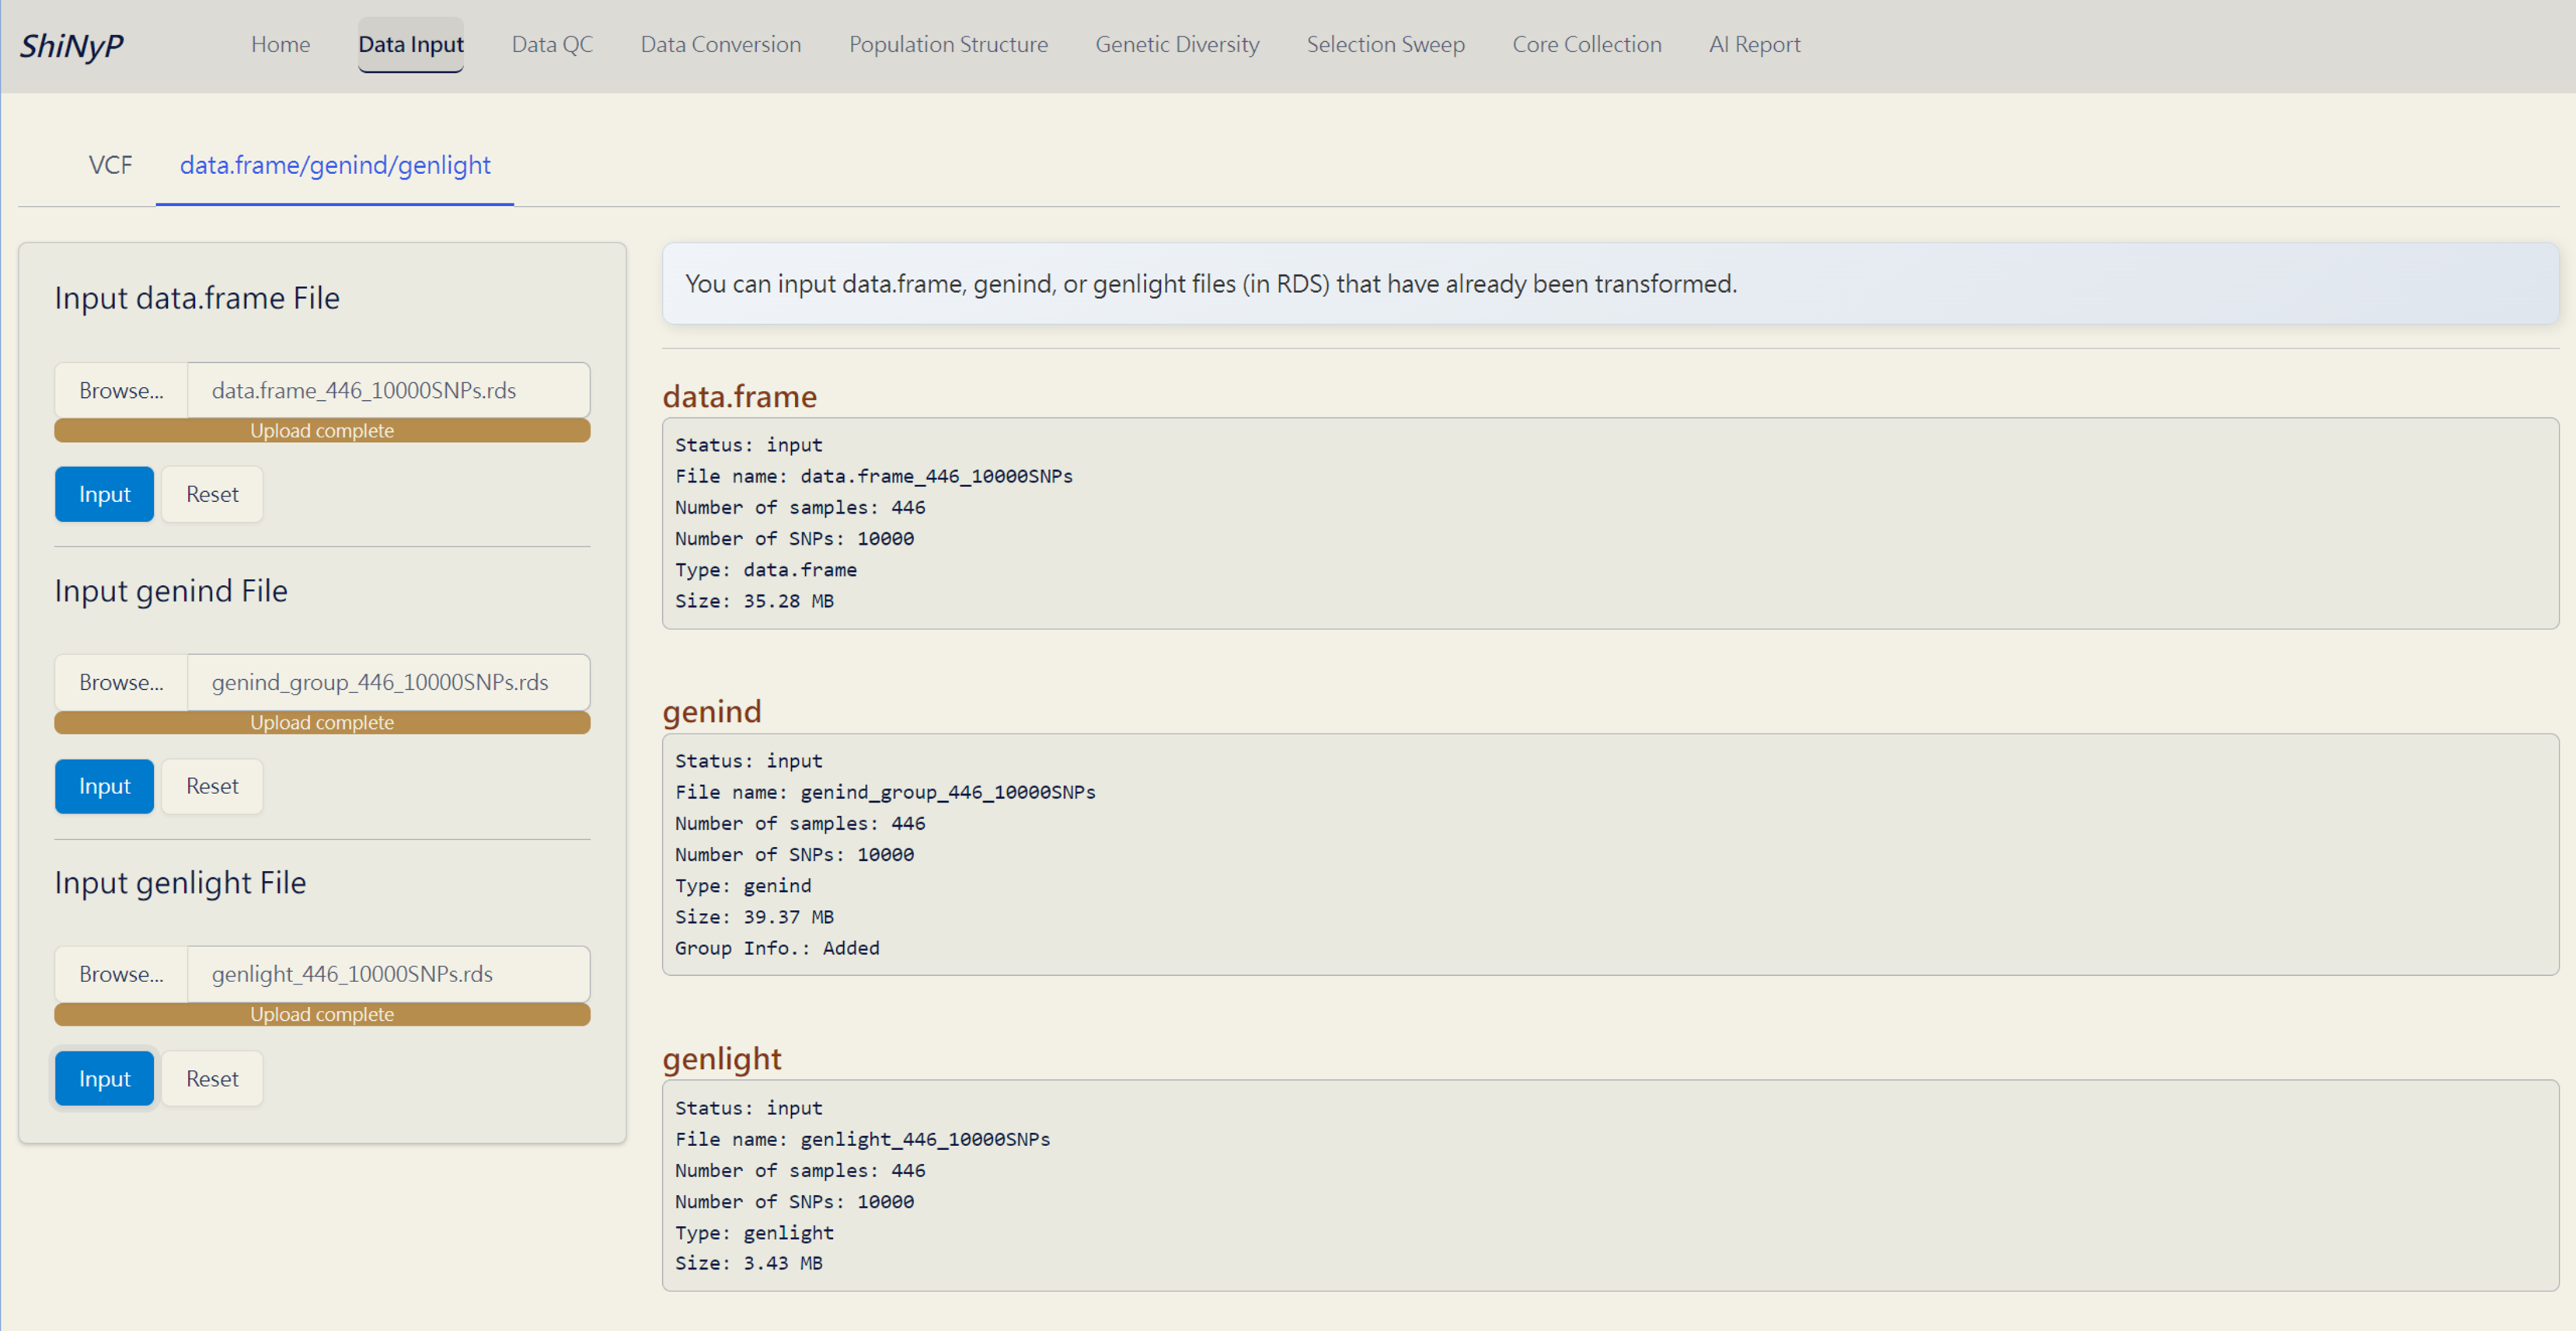
\includegraphics[width=8.33333in,height=\textheight]{images/圖片17.png}

{\textbf{\emph{\texttt{data.frame}}}}\emph{/{\textbf{\texttt{genind}}}/{\textbf{\texttt{genlight}}} Data Input!}

\chapter{Data QC}\label{sec-data-qc}

➡️ This section contains three subpages: \ul{\textbf{Sample QC}}, \ul{\textbf{SNP QC}}, and \ul{\textbf{SNP Density}}, allowing you to assess the quality of samples and SNPs in {\textbf{\texttt{data.frame}}}, as well as visualize SNP density across the genome.

\section{Sample QC}\label{sample-qc}

\paragraph*{Required Dataset (one of the following):}\label{required-dataset-one-of-the-following-1}
\addcontentsline{toc}{paragraph}{Required Dataset (one of the following):}

\begin{itemize}
\item
  {\textbf{\texttt{data.frame}}} file from the \ul{Data Input} page
\item
  SNP post-QC {\textbf{\texttt{data.frame}}} file from the subpage \ul{Data QC}/\ul{SNP QC}
\end{itemize}

\paragraph*{Step 1: Get Summary}\label{step-1-get-summary}
\addcontentsline{toc}{paragraph}{Step 1: Get Summary}

First, obtain the sample summary statistics (missing rate and heterozygosity rate) by clicking both {\textbf{Summary}} buttons and you will see the results.

\paragraph*{Step 2: Sample QC}\label{step-2-sample-qc}
\addcontentsline{toc}{paragraph}{Step 2: Sample QC}

Adjust the thresholds and click the {\textbf{Sample QC by Thresholds}} button. This will generate the Post-QC {\textbf{\texttt{data.frame}}} file.

\begin{quote}
\textbf{Note:} If you prefer not to perform sample QC by sample missing rate or heterozygosity rate, please set the threshold to 0.
\end{quote}

\paragraph*{Outputs:}\label{outputs-1}
\addcontentsline{toc}{paragraph}{Outputs:}

\begin{itemize}
\item
  \textbf{data.frame (RDS)}: Updated {\textbf{\texttt{data.frame}}} file. It's necessary for downstream analyses, \emph{please download and save it!}
\item
  \textbf{Site Info. (RDS)}: Updated SNP site information file. It's necessary for downstream analyses, \emph{please download and save it!}
\end{itemize}

\includegraphics[width=8.33333in,height=\textheight]{images/圖片19.png}

\emph{Sample QC Complete!}

\section{SNP QC}\label{snp-qc}

\paragraph*{Required Dataset (one of the following):}\label{required-dataset-one-of-the-following-2}
\addcontentsline{toc}{paragraph}{Required Dataset (one of the following):}

\begin{itemize}
\item
  {\textbf{\texttt{data.frame}}} file from the \ul{Data Input} page
\item
  Sample post-QC {\textbf{\texttt{data.frame}}} file from the subpage \ul{Data QC}/\ul{Sample QC}
\end{itemize}

\paragraph*{Step 1: Get Summary}\label{step-1-get-summary-1}
\addcontentsline{toc}{paragraph}{Step 1: Get Summary}

First, obtain the SNP summary statistics {[}missing rate, minor allele frequency (MAF), heterozygosity rate, and Hardy-Weinberg equilibrium (HWE){]} by clicking all {\textbf{Summary}} buttons and you will see the results.

\paragraph*{Step 2: Sample QC}\label{step-2-sample-qc-1}
\addcontentsline{toc}{paragraph}{Step 2: Sample QC}

Adjust the thresholds and click the {\textbf{SNP QC by Thresholds}} button. This will generate the Post-QC {\textbf{\texttt{data.frame}}} file.

\begin{quote}
\textbf{Note:} If you prefer not to perform QC based on SNP missing rate or heterozygosity rate, set the missing rate threshold to 1, the MAF to 0, and the heterozygosity rate to 0 and 1. Additionally, leave the `Do SNP QC by HWE' checkbox unticked to skip QC based on SNP HWE.
\end{quote}

\paragraph*{Outputs:}\label{outputs-2}
\addcontentsline{toc}{paragraph}{Outputs:}

\begin{itemize}
\item
  \textbf{data.frame (RDS)}: Updated {\textbf{\texttt{data.frame}}} file. It's necessary for downstream analyses, \emph{please download and save it!}
\item
  \textbf{Site Info. (RDS)}: Updated SNP site information file. It's necessary for downstream analyses, \emph{please download and save it!}
\end{itemize}

\includegraphics[width=8.33333in,height=\textheight]{images/圖片21.png}

\emph{SNP QC Complete!}

\section{SNP Density}\label{snp-density}

\paragraph*{Required Dataset (one of the following):}\label{required-dataset-one-of-the-following-3}
\addcontentsline{toc}{paragraph}{Required Dataset (one of the following):}

\begin{itemize}
\item
  \textbf{Site Info.} \textbf{(RDS)} of the current \textbf{\texttt{data.frame}}, downloadable from \ul{Data Input} or \ul{Data QC} pages.
\item
  \textbf{Chromosome Info.} \textbf{(CSV)}: Reference genome information of the current study.

  \textbf{\emph{Click here}}\emph{: Download an example of \textbf{Chromosome Info.(CSV)}.}

  ▼ Example: The \textbf{Chromosome Info.} of rice (Data source: https://www.ncbi.nlm.nih.gov/datasets/genome/GCF\_034140825.1/)

  \begin{longtable}[]{@{}lll@{}}
  \toprule\noalign{}
  Chr & Start & End \\
  \midrule\noalign{}
  \endhead
  \bottomrule\noalign{}
  \endlastfoot
  Chr01 & 0 & 43929697 \\
  Chr02 & 0 & 36447916 \\
  Chr03 & 0 & 37399924 \\
  Chr04 & 0 & 36078568 \\
  Chr05 & 0 & 30400764 \\
  Chr06 & 0 & 32122276 \\
  Chr07 & 0 & 29936421 \\
  Chr08 & 0 & 28605474 \\
  Chr09 & 0 & 27474823 \\
  Chr10 & 0 & 23931887 \\
  Chr11 & 0 & 31111469 \\
  Chr12 & 0 & 28271460 \\
  \end{longtable}
\end{itemize}

\paragraph*{Steps:}\label{steps}
\addcontentsline{toc}{paragraph}{Steps:}

\begin{enumerate}
\def\labelenumi{\arabic{enumi}.}
\item
  {Upload} \textbf{Site Info.} \textbf{(RDS)} and \textbf{Chromosome Info. (CSV)}.
\item
  Choose a window size in kilobases (kb).
\item
  Click the {\textbf{Summary}} button. This will calculate the density of SNPs across the genome.
\end{enumerate}

\paragraph*{Outputs:}\label{outputs-3}
\addcontentsline{toc}{paragraph}{Outputs:}

\begin{itemize}
\item
  \textbf{SNP Density Plot (PDF):} An ideogram visualizing SNP density across the genome within a defined window size. A gradient color palette is used to represent varying SNP densities: \emph{green} for \ul{lower densities}, \emph{yellow} for \ul{medium densities}, and \emph{red} for \ul{higher densities}, with \emph{grey} indicating regions with \ul{zero SNP}.
\item
  \textbf{SNP Density (CSV):} A table detailing SNP density across each chromosome. \emph{bp\_over\_SNPs}: The total base pairs (bp) per SNP in each window, representing the average spacing between SNPs. \emph{SNPs\_over\_1000bp}: The number of SNPs per 1,000 base pairs, providing a normalized measure of SNP density across the genome.
\end{itemize}

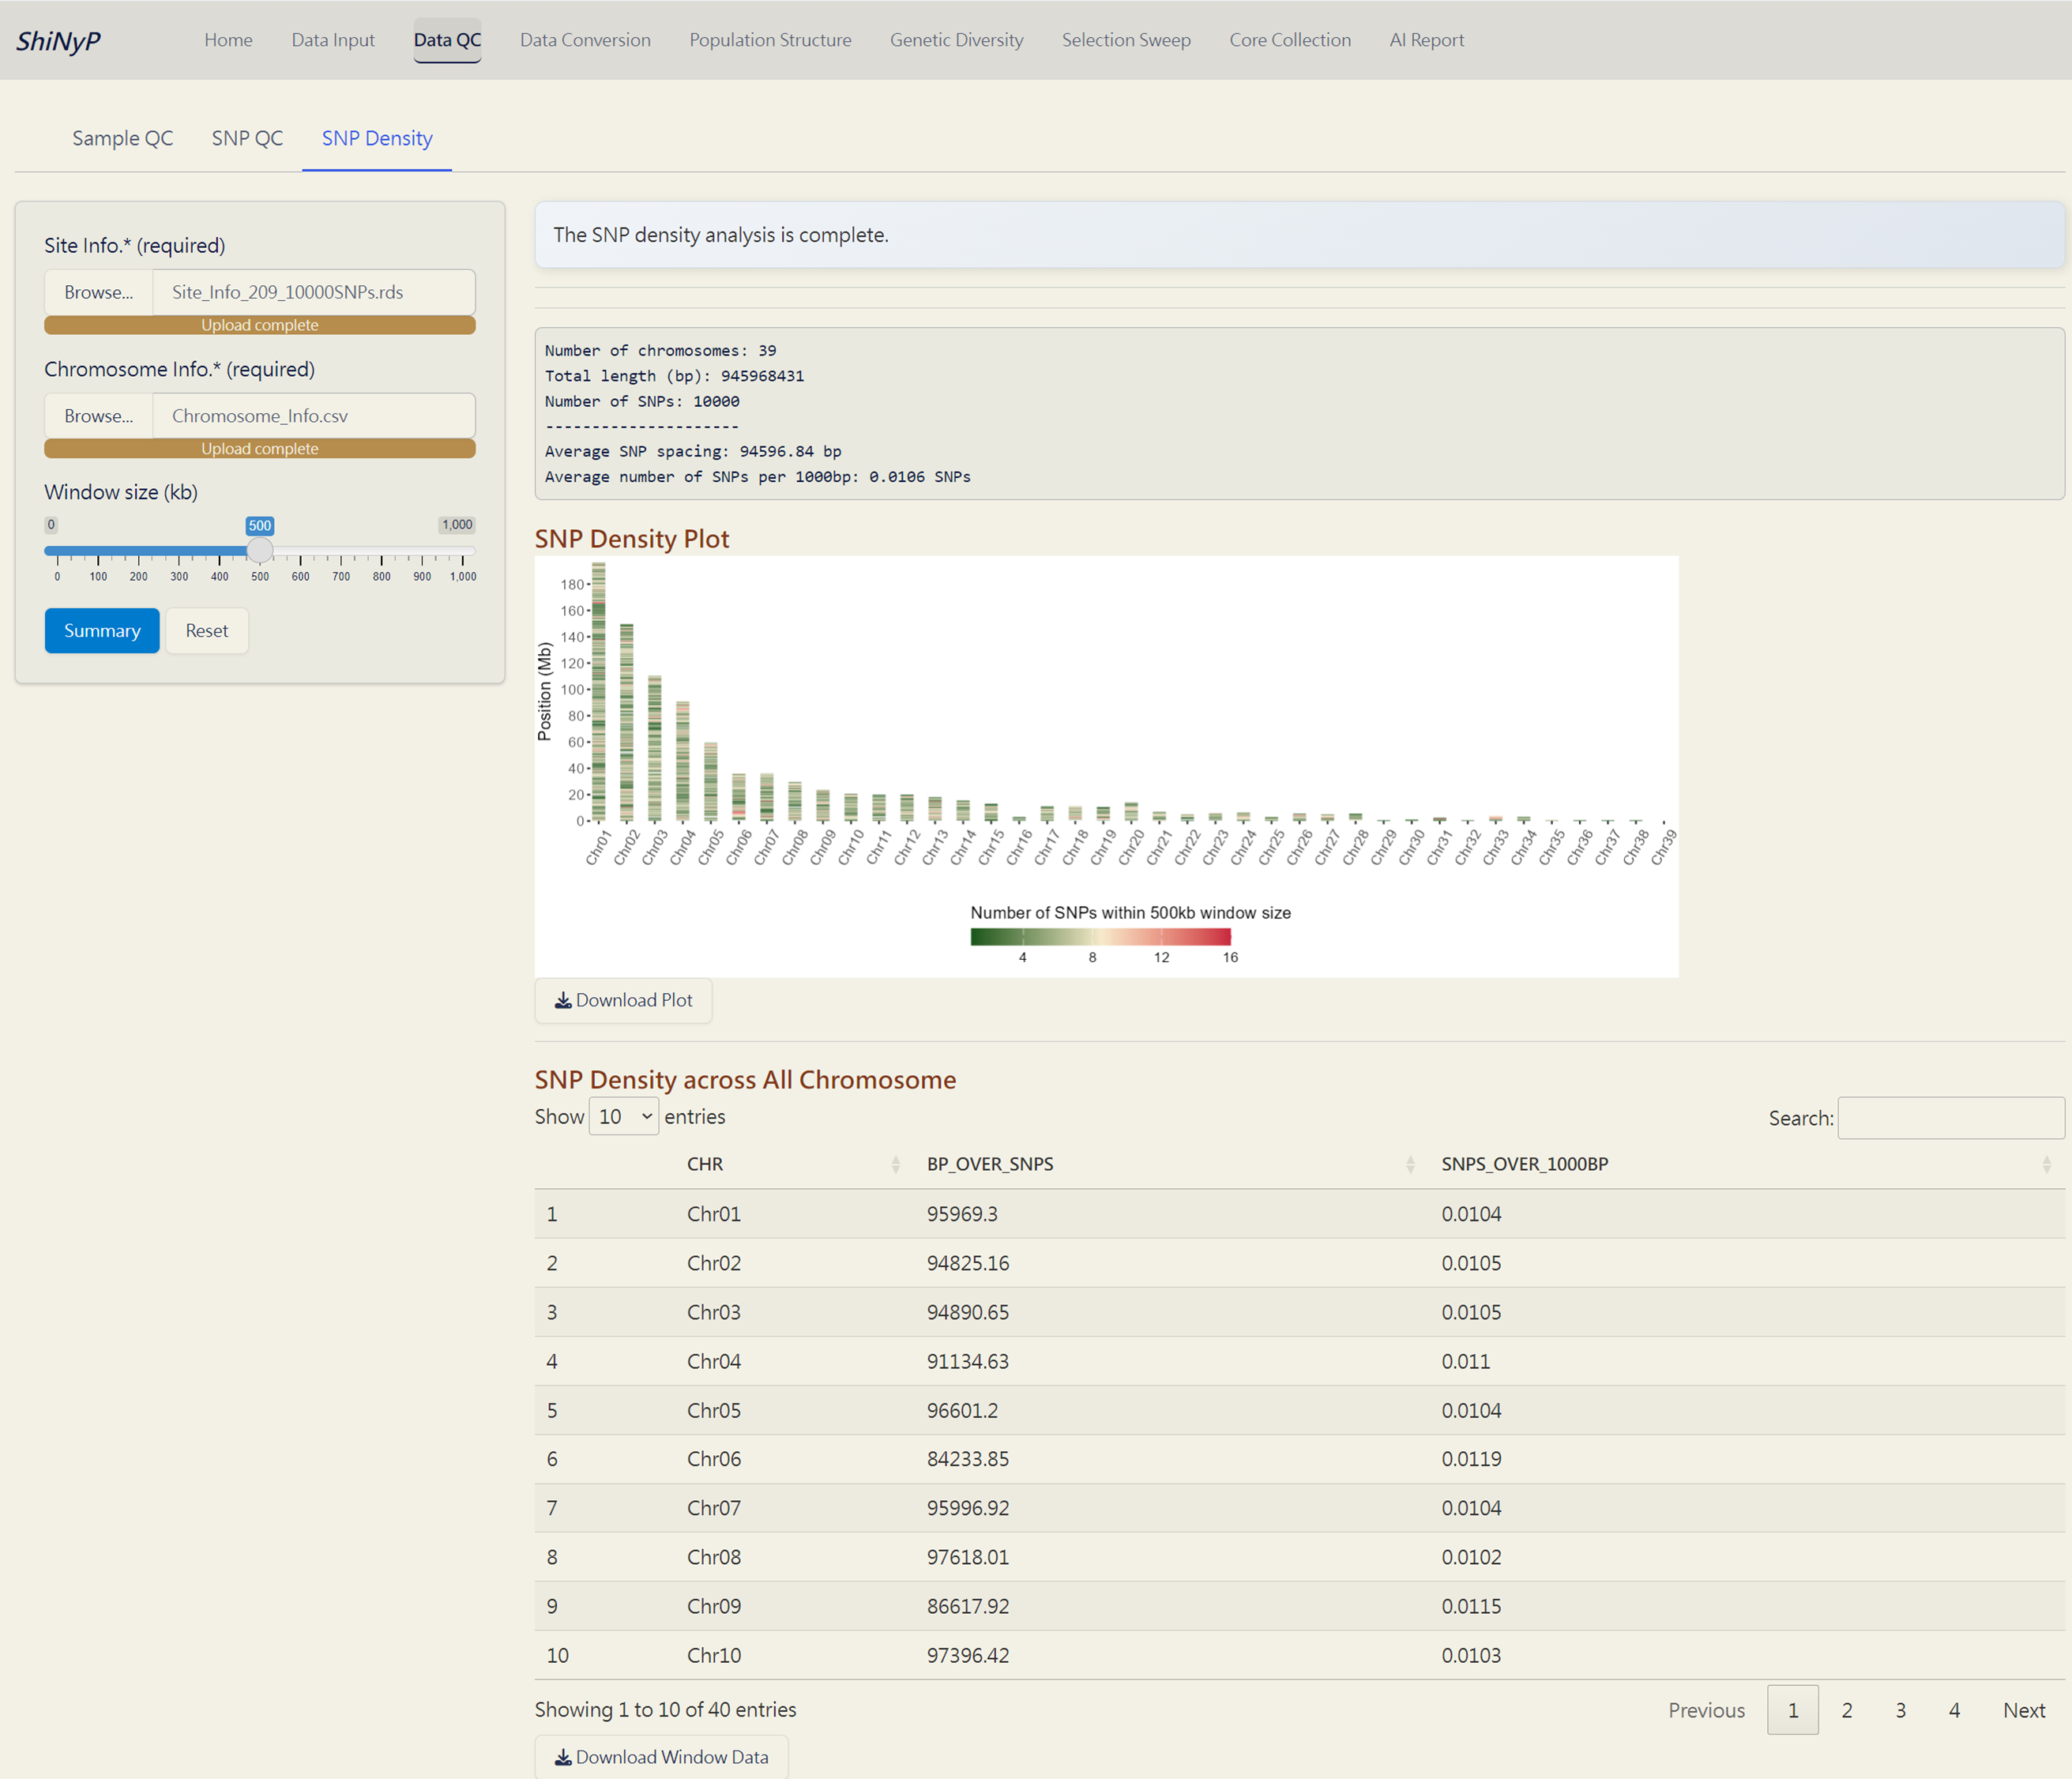
\includegraphics[width=8.33333in,height=\textheight]{images/clipboard-3331950775.png}

\emph{SNP Density Complete!}

\chapter{Data Transform}\label{sec-data-conversion}

➡️ This section allow you to convert your SNP data in {\textbf{\texttt{data.frame}}} into {\textbf{\texttt{genind}}} and {\textbf{\texttt{genlight}}}.

\paragraph*{Required Dataset (one of the following):}\label{required-dataset-one-of-the-following-4}
\addcontentsline{toc}{paragraph}{Required Dataset (one of the following):}

\begin{itemize}
\item
  Input VCF Data ({\textbf{\texttt{data.frame}}} file) from the \ul{Data Input} page.
\item
  Post-QC Data ({\textbf{\texttt{data.frame}}} file) from the \ul{Data QC} page.
\end{itemize}

\paragraph*{\texorpdfstring{Step 1: Transform {\textbf{\texttt{data.frame}}} to {\textbf{\texttt{genind}}}}{Step 1: Transform data.frame to genind}}\label{step-1-transform-data.frame-to-genind}
\addcontentsline{toc}{paragraph}{Step 1: Transform {\textbf{\texttt{data.frame}}} to {\textbf{\texttt{genind}}}}

Click the {\textbf{Transform to genind}} button. This will generate the {\textbf{\texttt{genind}}} file.

\begin{quote}
\textbf{Note:} After obtaining the clustering results from the \ul{Population Structure}/\ul{DAPC} subpage, you can add \textbf{Group Info.} to the {\textbf{\texttt{genind}}} file by inputting the `\textbf{DAPC\_Group\_Info.csv}'. This step is necessary for analyses like `Genetic Distance' and `AMOVA'.
\end{quote}

\paragraph*{\texorpdfstring{Step 2: Transform {\textbf{\texttt{genind}}} to {\textbf{\texttt{genlight}}}}{Step 2: Transform genind to genlight}}\label{step-2-transform-genind-to-genlight}
\addcontentsline{toc}{paragraph}{Step 2: Transform {\textbf{\texttt{genind}}} to {\textbf{\texttt{genlight}}}}

Click the {\textbf{Transform to genlight}} button. This will generate the {\textbf{\texttt{genlight}}} file.

\paragraph*{Outputs:}\label{outputs-4}
\addcontentsline{toc}{paragraph}{Outputs:}

\begin{itemize}
\item
  \textbf{genind (RDS)}: {\textbf{\texttt{genind}}} file. It's necessary for downstream analyses, \emph{please download and save it!}
\item
  \textbf{genlight (RDS)}: {\textbf{\texttt{genlight}}} file. It's necessary for downstream analyses, \emph{please download and save it!}
\end{itemize}

\begin{quote}
\textbf{Note:} Please download and save your {\textbf{\texttt{data.frame}}}, {\textbf{\texttt{genind}}}, and {\textbf{\texttt{genlight}}} files after transformation. This will save you from having to input the large VCF file again next time.
\end{quote}

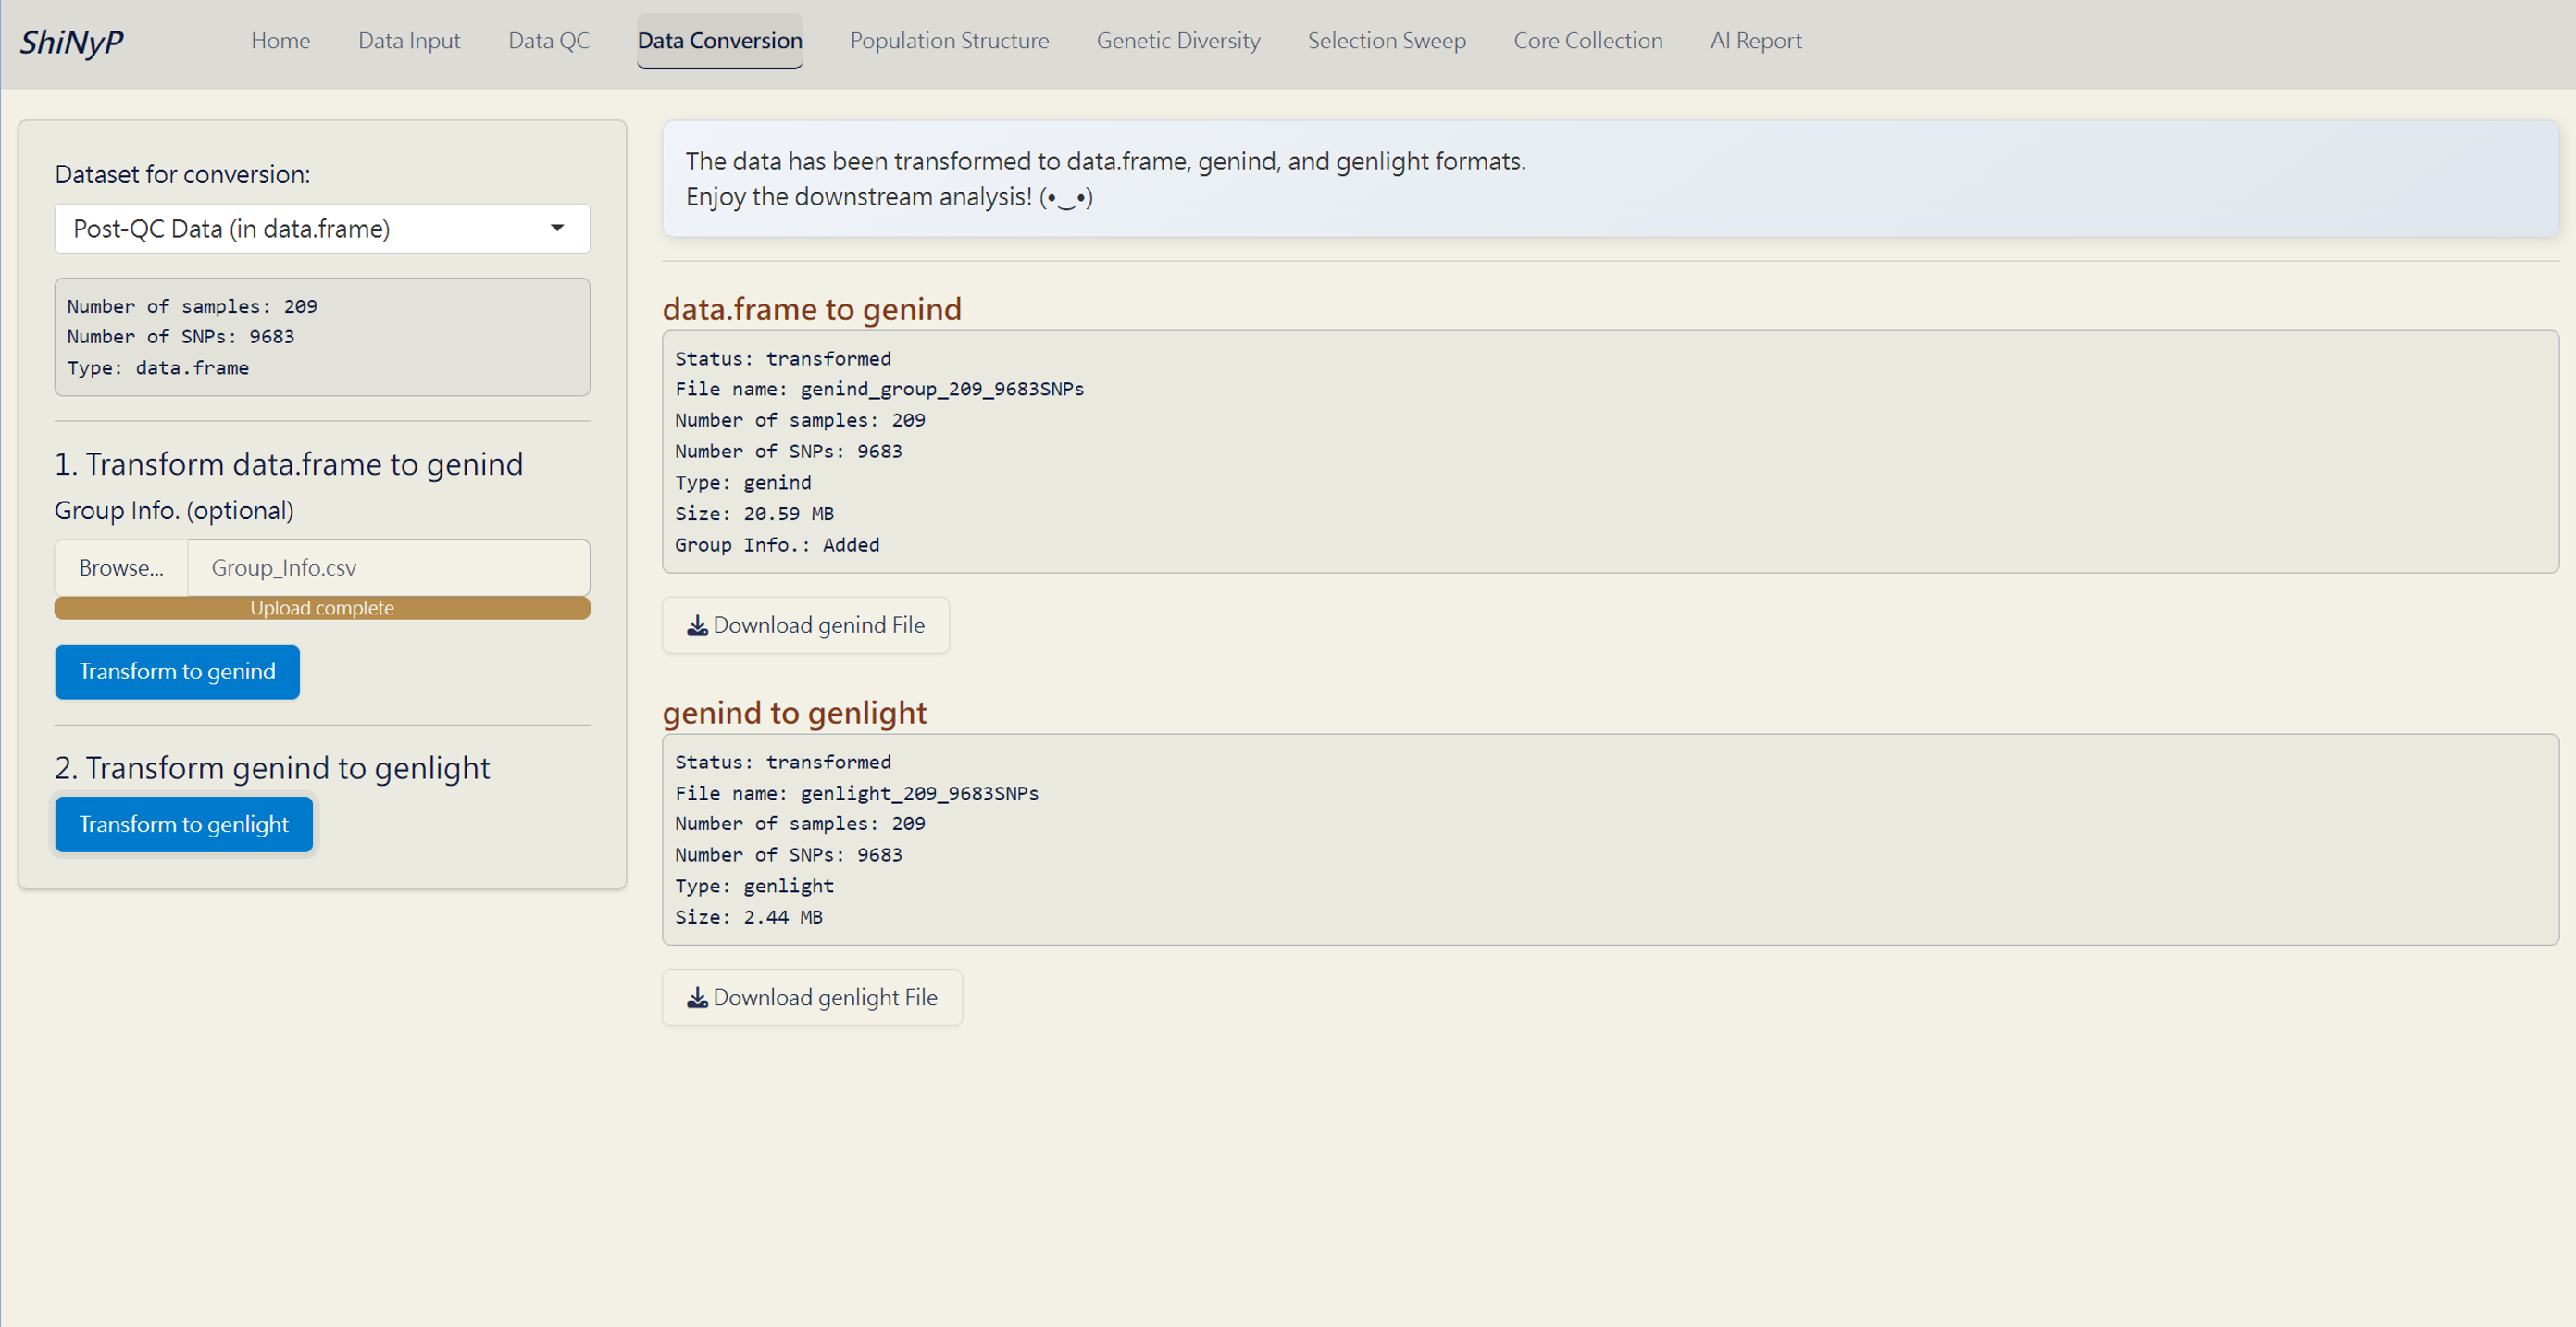
\includegraphics{images/圖片22.png}

\emph{Data Transformation Complete!}

\chapter{Population Structure}\label{sec-population-structure}

➡️ This section contains seven subpages: \ul{\textbf{PCA}}, \ul{\textbf{DAPC}}, \ul{\textbf{UPGMA Tree}}, \ul{\textbf{NJ Tree}}, \ul{\textbf{Kinship}}, \ul{\textbf{Scatter Plot}}\textsuperscript{\textbf{Plus}}, and \ul{\textbf{Tree Plot}}\textsuperscript{\textbf{Plus}} allowing you to conduct various population structure analyses and customize your plot.

\includegraphics{images/Supp. Fig. 1-5_頁面_2.jpg}

\section{PCA (Principal Component Analysis)}\label{pca-principal-component-analysis}

A widely used method to uncover underlying population structure by reducing the dimensionality of genetic data.

\paragraph*{Required Dataset:}\label{required-dataset-1}
\addcontentsline{toc}{paragraph}{Required Dataset:}

\begin{itemize}
\tightlist
\item
  {\textbf{\texttt{data.frame}}}
\end{itemize}

\paragraph*{\texorpdfstring{\textbf{One Step:}}{One Step:}}\label{one-step-1}
\addcontentsline{toc}{paragraph}{\textbf{One Step:}}

\begin{enumerate}
\def\labelenumi{\arabic{enumi}.}
\tightlist
\item
  Click the {\textbf{Run PCA}} button to generate PCA plots and the following downloadable files.
\end{enumerate}

\begin{quote}
\textbf{Note}: You can upload the \textbf{Group Info.} (from \ul{Population Structure}/\ul{DAPC}) or \textbf{Core Sample Info.} (from \ul{Core Collection}/\ul{Core Sample Set}) to classify individuals and color them in the PCA Scatter Plot.
\end{quote}

\paragraph*{Outputs:}\label{outputs-5}
\addcontentsline{toc}{paragraph}{Outputs:}

\begin{itemize}
\item
  \textbf{PCA Scatter Plot (PDF)}: A scatter plot showing the distribution of samples based on principal components, with each dot representing an individual.
\item
  \textbf{PC Explained Variance Plot (PDF)}: Visualizes the variance explained by each principal component.
\item
  \textbf{Explained Variance (CSV)}: Contains the explained variance of each principal component.
\item
  \textbf{PCA Transformed Data (CSV)}: Dataset transformed into principal components, with samples as rows and principal components as columns.
\item
  \textbf{PCA Object (RDS)}: Contains all PCA results for future use and reproducibility, and can be used as input data in the \ul{Population Structure}/\ul{Scatter Plot}\textsuperscript{Plus} subpage.
\end{itemize}

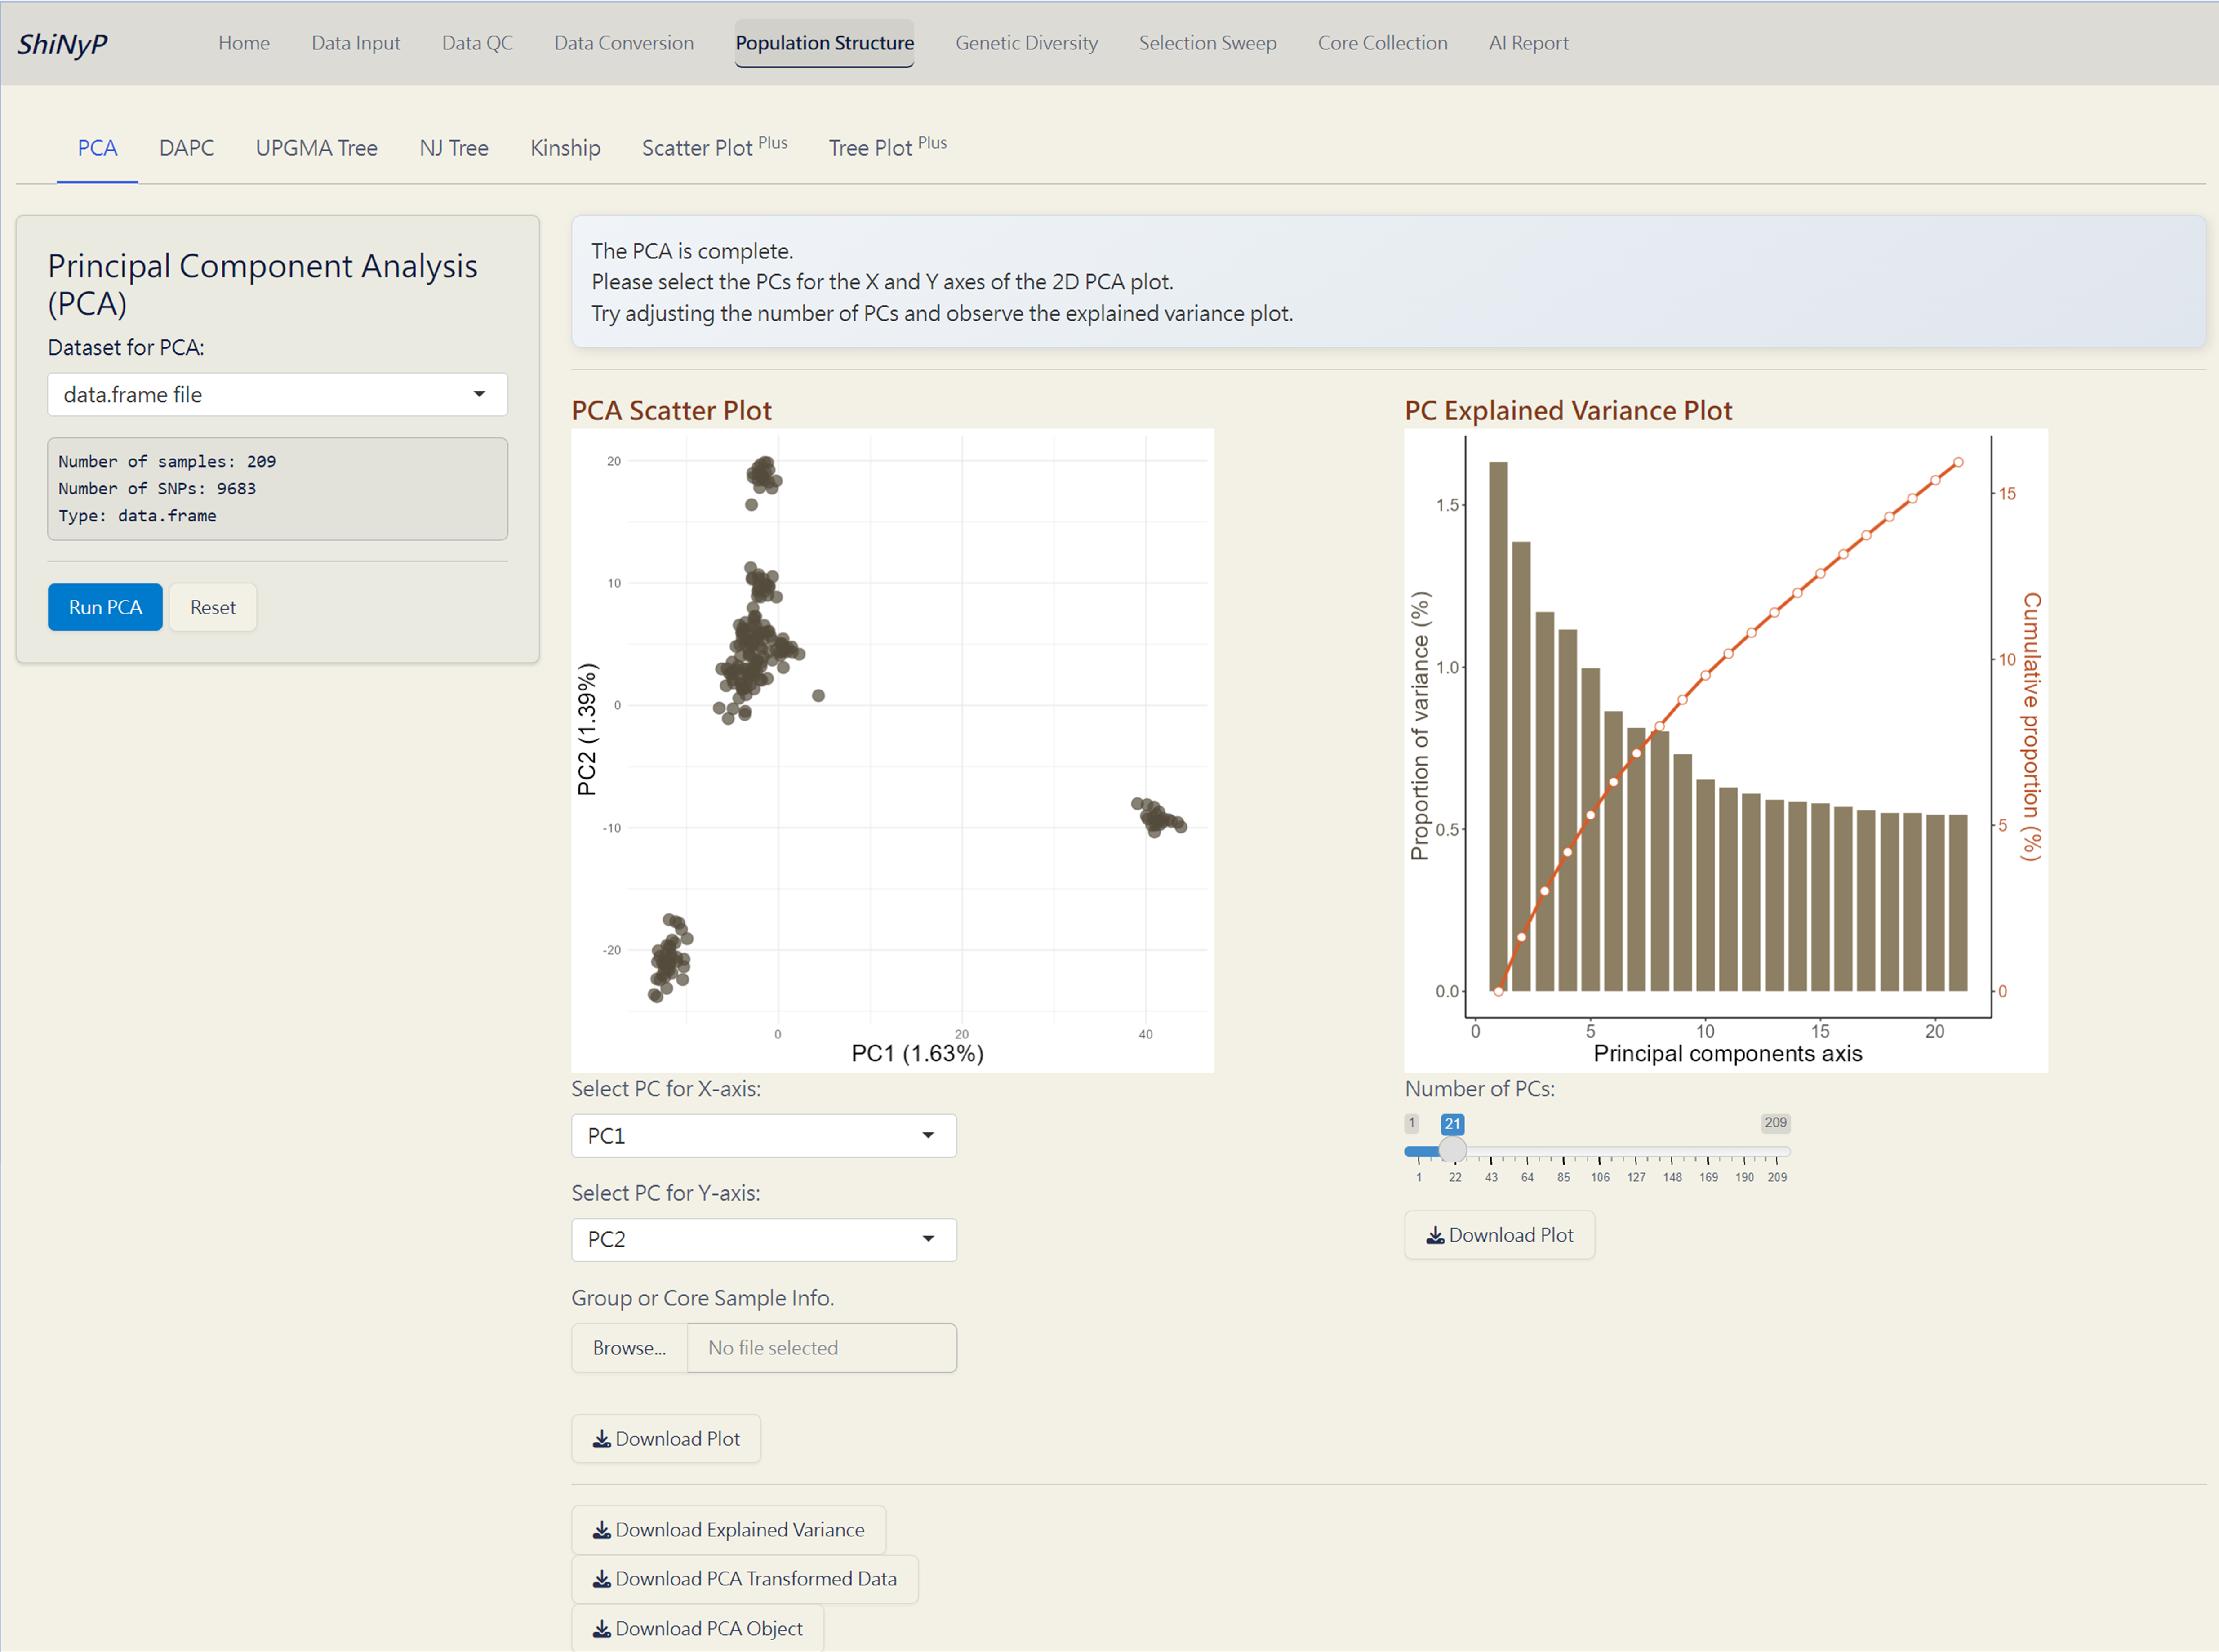
\includegraphics{images/clipboard-534056671.png}

\emph{PCA Complete!}

\section{DAPC (Discriminant Analysis of Principal Components)}\label{dapc-discriminant-analysis-of-principal-components}

A multivariate method for identifying and visualizing genetic clusters by combining PCA and Linear Discriminant Analysis (LDA) \citep{jombart2010}. For more information, visit https://adegenet.r-forge.r-project.org/files/tutorial-dapc.pdf.

\paragraph*{Required Dataset:}\label{required-dataset-2}
\addcontentsline{toc}{paragraph}{Required Dataset:}

\begin{itemize}
\tightlist
\item
  {\textbf{\texttt{genind}}}
\end{itemize}

\paragraph*{\texorpdfstring{Step 1: \textbf{Cluster Identification}}{Step 1: Cluster Identification}}\label{step-1-cluster-identification}
\addcontentsline{toc}{paragraph}{Step 1: \textbf{Cluster Identification}}

\begin{enumerate}
\def\labelenumi{\arabic{enumi}.}
\tightlist
\item
  Click the {\textbf{Run DAPC I}} button to determine the optimal number of clusters (the lowest BIC value indicates the optimal number of clusters).
\end{enumerate}

\begin{quote}
\textbf{Note:} The default number of PC axes for cluster identification is set to retain PCs that capture up to 80\% of the total variance. You can refer the ``PC Explained Variance Plot'' in the \ul{Population Structure}/\ul{PCA} subpage.
\end{quote}

\paragraph*{\texorpdfstring{Step 2: \textbf{DAPC Analysis}}{Step 2: DAPC Analysis}}\label{step-2-dapc-analysis}
\addcontentsline{toc}{paragraph}{Step 2: \textbf{DAPC Analysis}}

\begin{enumerate}
\def\labelenumi{\arabic{enumi}.}
\item
  Choose the number of cluster (K) based on the ``Bayesian Information Criterion (BIC) Plot''.
\item
  Click the {\textbf{Run DAPC II}} button to generate DAPC plots and the following downloadable files.
\end{enumerate}

\begin{quote}
\textbf{Note}: You can download the ``DAPC Object'' and upload it on \ul{Population Structure}/\ul{Scatter Plot}\textsuperscript{Plus} subpage to customize your 2D and 3D scatter plots.
\end{quote}

\paragraph*{Outputs:}\label{outputs-6}
\addcontentsline{toc}{paragraph}{Outputs:}

\begin{itemize}
\item
  \textbf{Bayesian Information Criterion (BIC) Plot (PDF)}: Visual representation of the BIC for model selection.
\item
  \textbf{Density Plot of First \& Second Discriminant Function} \textbf{(PDF)}: Displays the density of the first and second discriminant functions, with each row bar representing an individual.
\item
  \textbf{DAPC Scatter Plot (PDF)}: A scatter plot showing the distribution of samples based on discriminant functions (x-axis: first discriminant function; y-axis: second discriminant function), with each dot representing an individual.
\item
  \textbf{DAPC Membership Probability Plot (PDF)}: Visualizes membership probabilities of individuals in different groups, with each row bar representing an individual.
\item
  \textbf{DAPC Group Info. (CSV)}: Contains the group assignments for each individual based on DAPC. This file used in various subpages.
\item
  \textbf{DAPC Transformed Data (CSV)}: Dataset transformed into discriminant functions with samples as rows and discriminant functions as columns.
\item
  \textbf{DAPC Object (RDS)}: Contains all results from the DAPC analysis for future reproducibility. It can be used as input data in the \ul{Population Structure}/\ul{Scatter Plot}\textsuperscript{Plus} and \ul{Core Collection}/\ul{Core SNP Set} subpages.
\end{itemize}

\includegraphics{images/clipboard-1914132278.png}

\emph{DAPC Complete!}

\section{UPGMA (Unweighted Pair Group Method with Arithmetic mean) Tree}\label{upgma-unweighted-pair-group-method-with-arithmetic-mean-tree}

A classic approaach for constructing rooted trees based on genetic distance data. UPGMA tree is generated by \emph{poppr} and \emph{ggtree} packages \citep{yu2016, kamvar2014}.

\paragraph*{Required Dataset:}\label{required-dataset-3}
\addcontentsline{toc}{paragraph}{Required Dataset:}

\begin{itemize}
\tightlist
\item
  {\textbf{\texttt{genlight}}}
\end{itemize}

\paragraph*{\texorpdfstring{\textbf{Steps}:}{Steps:}}\label{steps-1}
\addcontentsline{toc}{paragraph}{\textbf{Steps}:}

\begin{enumerate}
\def\labelenumi{\arabic{enumi}.}
\item
  Choose the number of bootstrap replicates, which will be used for assessing the confidence of the branching structure.
\item
  Click the {\textbf{Run UPGMA}} button to generate tree plot.
\end{enumerate}

\begin{quote}
\textbf{Note}: You can download the ``UPGMA Object'' and upload it on \ul{Population Structure}/\ul{Tree Plot}\textsuperscript{Plus} subpage to customize your phylogenetic tree.
\end{quote}

\paragraph*{Outputs:}\label{outputs-7}
\addcontentsline{toc}{paragraph}{Outputs:}

\begin{itemize}
\item
  \textbf{UPGMA Phylogenetic Tree (PDF)}: A UPGMA rooted tree with a user-defined layout style.
\item
  \textbf{UPGMA Object (RDS)}: Contains all information of the UPGMA tree, and can be used as input data in the \ul{Population Structure}/\ul{Tree Plot}\textsuperscript{Plus} subpage.
\end{itemize}

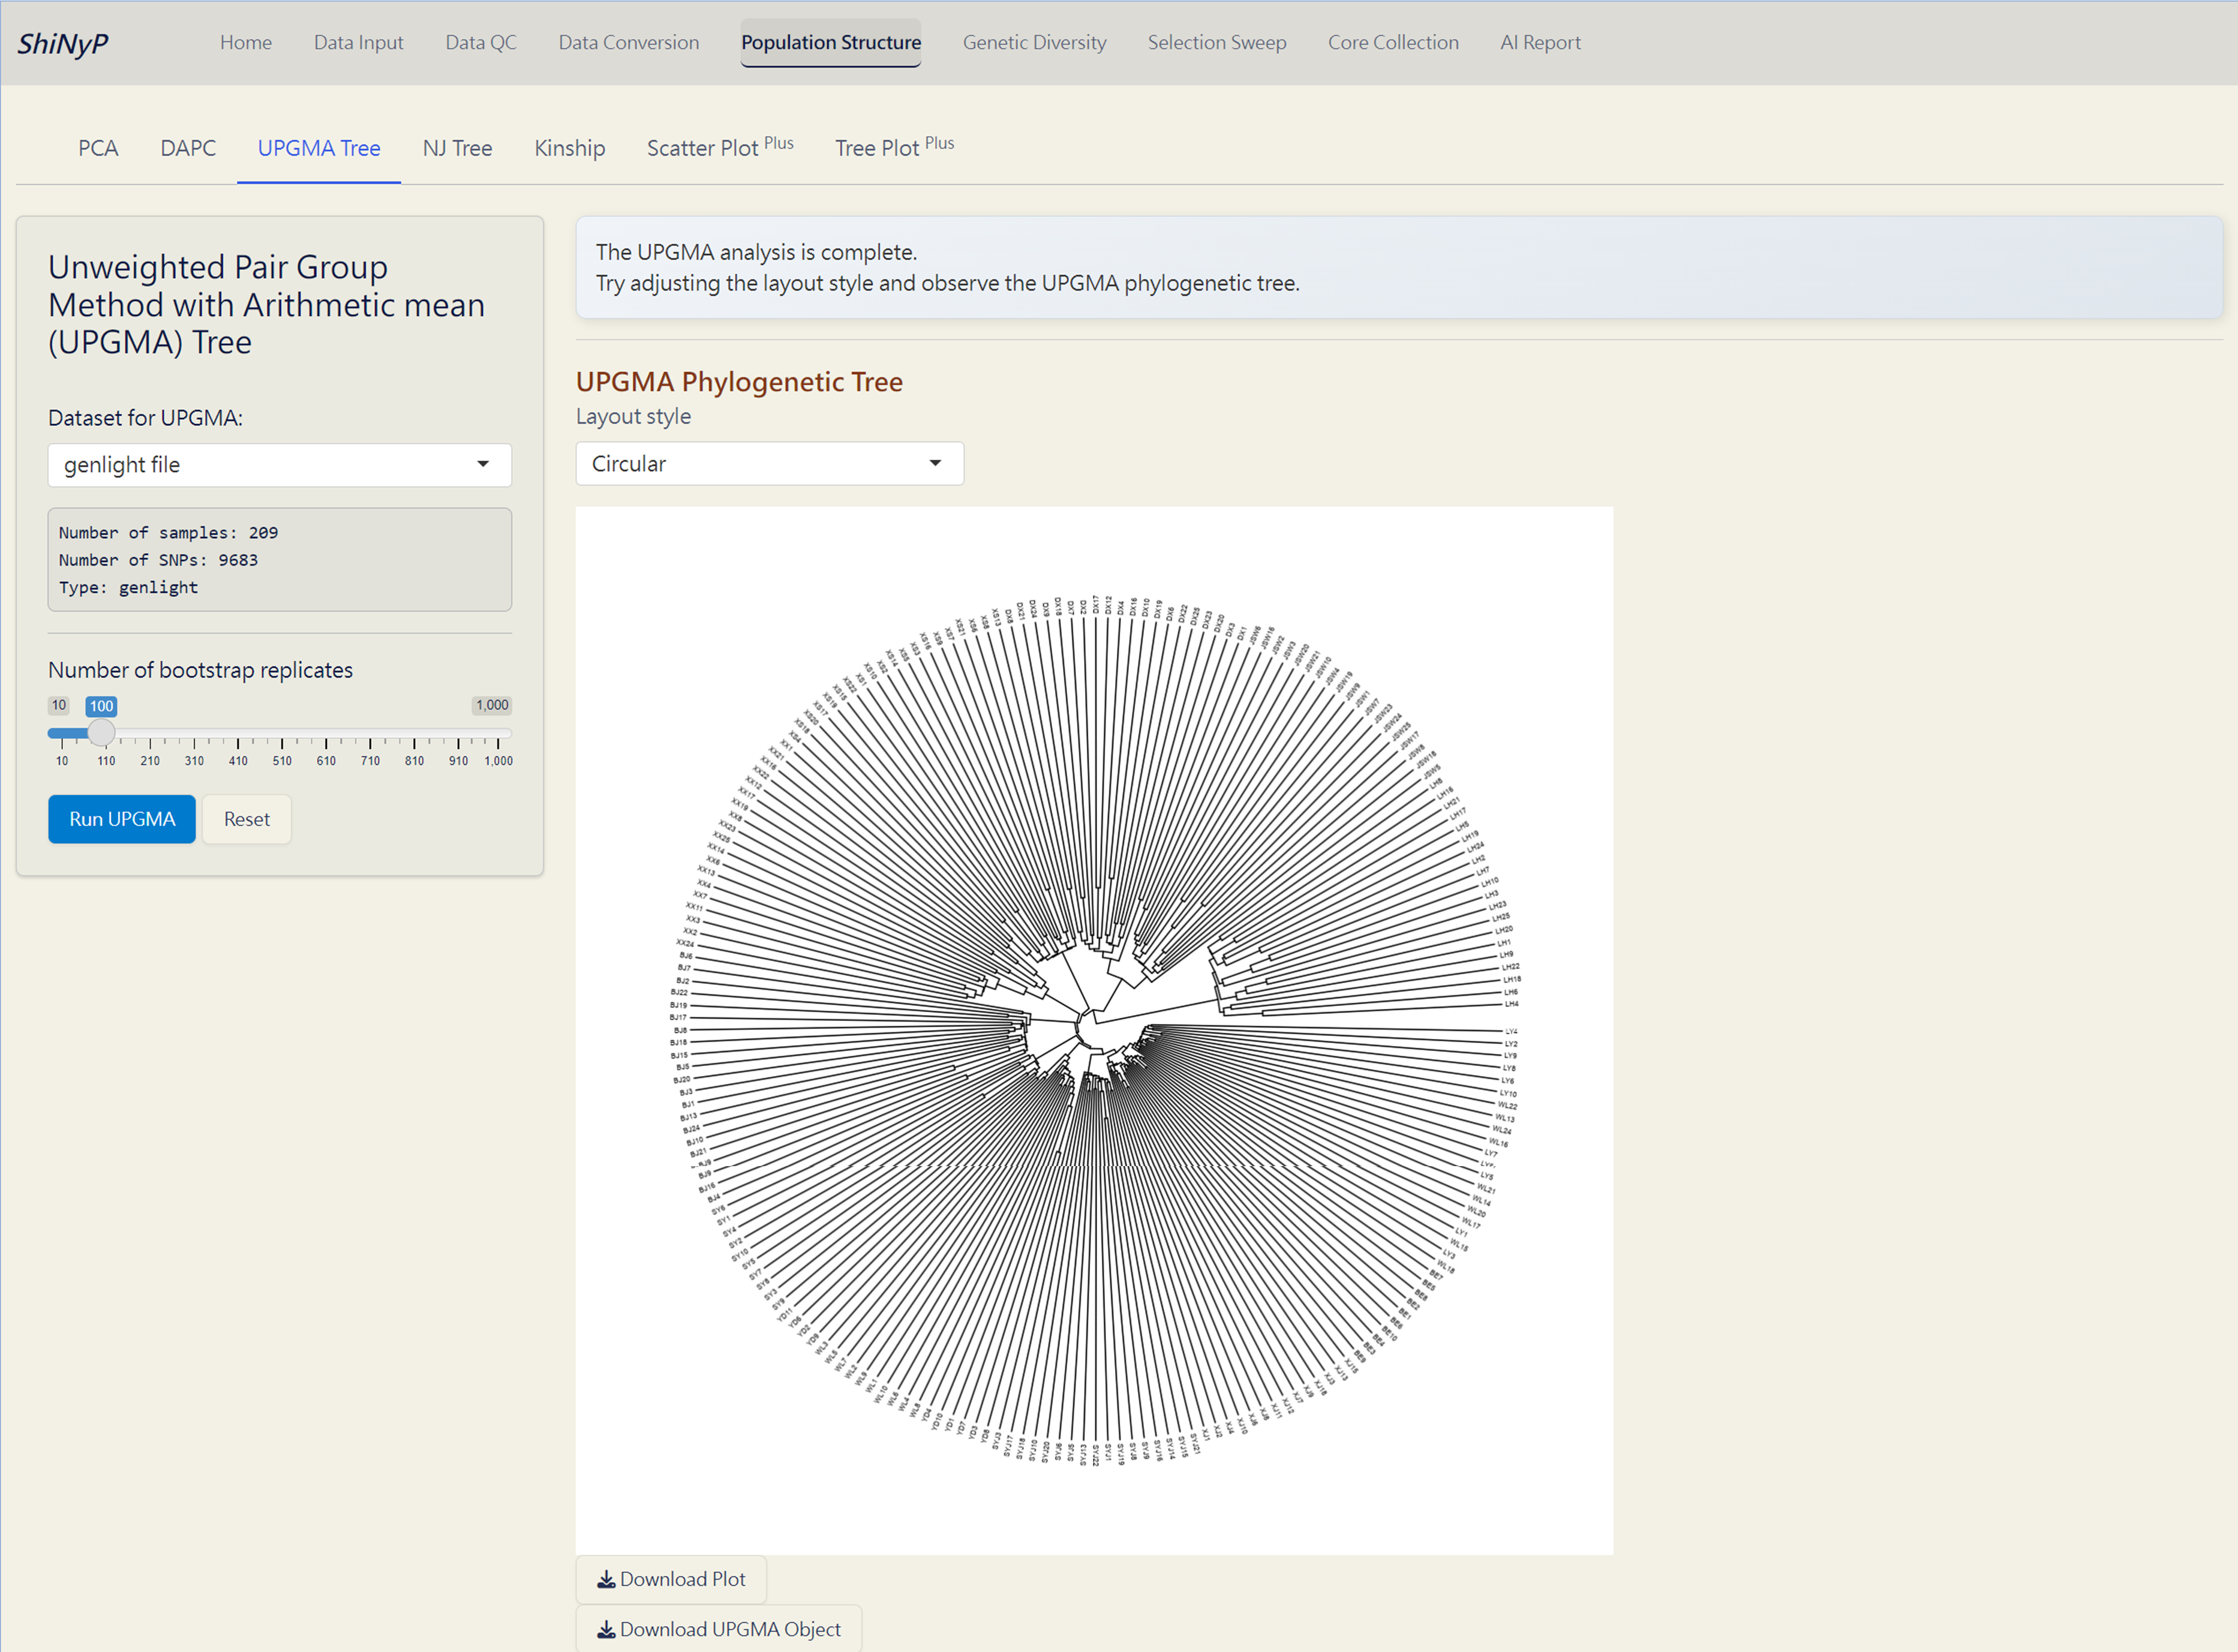
\includegraphics{images/clipboard-3531175086.png}

\emph{UPGMA Tree Complete!}

\section{NJ (Neighbor-Joining) Tree}\label{nj-neighbor-joining-tree}

A method for building unrooted trees using genetic distance data. NJ tree is generated by \emph{ape} and \emph{ggtree} packages \citep{paradis2018, yu2016}.

\paragraph*{Required Dataset:}\label{required-dataset-4}
\addcontentsline{toc}{paragraph}{Required Dataset:}

\begin{itemize}
\tightlist
\item
  {\textbf{\texttt{genlight}}}
\end{itemize}

\paragraph*{\texorpdfstring{\textbf{One Step:}}{One Step:}}\label{one-step-2}
\addcontentsline{toc}{paragraph}{\textbf{One Step:}}

\begin{enumerate}
\def\labelenumi{\arabic{enumi}.}
\tightlist
\item
  Click the {\textbf{Run NJ}} button to generate tree plot.
\end{enumerate}

\begin{quote}
\textbf{Note}: You can download the ``NJ Object'' and upload it on \ul{Population Structure}/\ul{Tree Plot}\textsuperscript{Plus} subpage to customize your phylogenetic tree.
\end{quote}

\paragraph*{Outputs:}\label{outputs-8}
\addcontentsline{toc}{paragraph}{Outputs:}

\begin{itemize}
\item
  \textbf{NJ Phylogenetic Tree (PDF)}: A NJ unrooted tree with a user-defined layout style.
\item
  \textbf{NJ Object (RDS)}: Contains all information of the NJ tree, and can be used as input data in the \ul{Population Structure}/\ul{Tree Plot}\textsuperscript{Plus} subpage.
\end{itemize}

\includegraphics{images/clipboard-1096590194.png}

\emph{NJ Tree Complete!}

\section{Kinship Analysis}\label{kinship-analysis}

A statistical method for assessing genetic relationships and relatedness among individuals based on shared alleles \citep{kang2010}. Kinship matrix is generated by \emph{statgenGWAS} package.For more information, visit https://rdrr.io/cran/statgenGWAS/man/kinship.html.

\paragraph*{Required Dataset:}\label{required-dataset-5}
\addcontentsline{toc}{paragraph}{Required Dataset:}

\begin{itemize}
\tightlist
\item
  {\textbf{\texttt{data.frame}}}
\end{itemize}

\paragraph*{\texorpdfstring{\textbf{Steps:}}{Steps:}}\label{steps-2}
\addcontentsline{toc}{paragraph}{\textbf{Steps:}}

\begin{enumerate}
\def\labelenumi{\arabic{enumi}.}
\item
  {Upload} \textbf{Group Info.} from \ul{Population Structure}/\ul{DAPC} (optional). If uploaded, the order of samples will follow the group assignment; otherwise, it will follow the order of the original VCF data.
\item
  Choose a method to run kinship analysis.
\item
  Click the {\textbf{Run Kinship}} button to generate the kinship matrix.
\end{enumerate}

\paragraph*{Outputs:}\label{outputs-9}
\addcontentsline{toc}{paragraph}{Outputs:}

\begin{itemize}
\item
  \textbf{Kinship Matrix Plot (PDF)}: A visual representation of the kinship matrix.
\item
  \textbf{Kinship Matrix (RDS)}: Contains the kinship matrix data.
\end{itemize}

\begin{quote}
Note: This kinship matrix can be directly used as input for \emph{GAPIT} package in genome-wide association studies (GWAS), helping to control for confounding effects.
\end{quote}

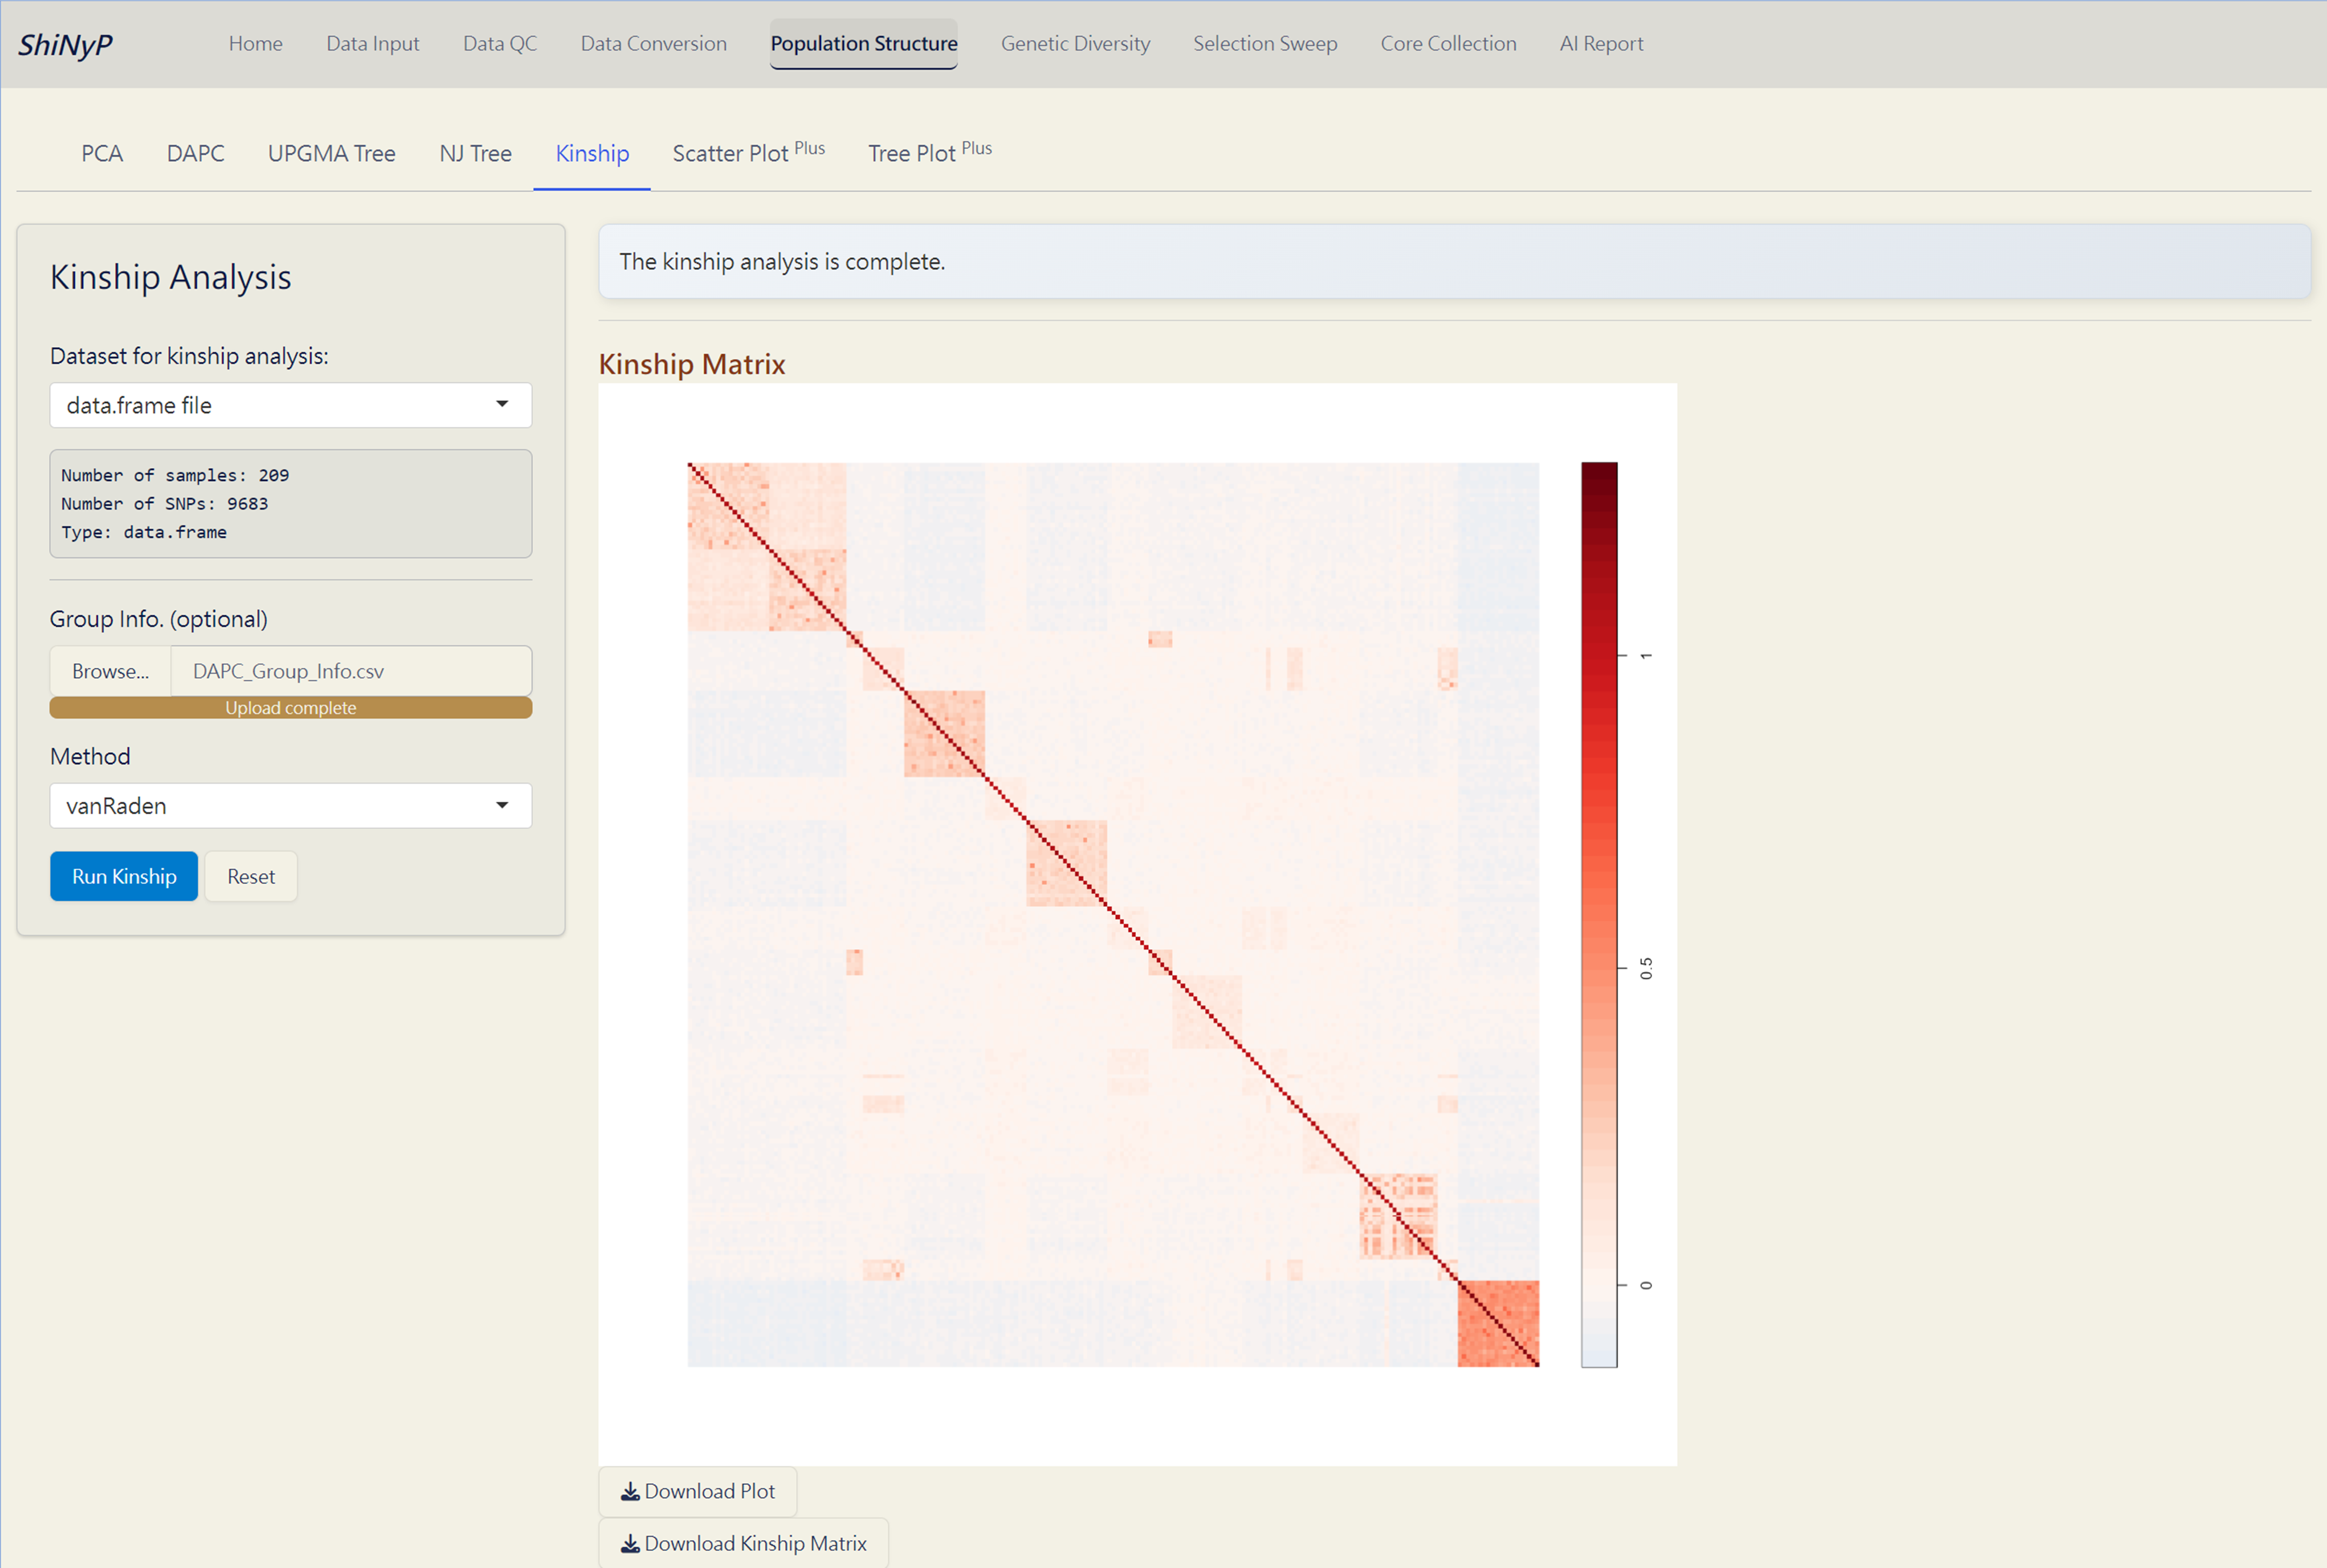
\includegraphics{images/clipboard-2215706632.png}

\emph{Kinship Analysis Complete!}

\section{\texorpdfstring{Scatter Plot \textsuperscript{Plus}}{Scatter Plot Plus}}\label{scatter-plot-plus}

Customize your scatter plot based on the results from \ul{Population Structure}/\ul{PCA} or \ul{Population Structure}/\ul{DAPC}.

\paragraph*{Required Files:}\label{required-files}
\addcontentsline{toc}{paragraph}{Required Files:}

\begin{itemize}
\tightlist
\item
  \textbf{PCA Object} (PCA\_prcomp\_Object.rds file) or \textbf{DAPC Object} (DAPC\_dapc\_Object.rds file)
\item
  \textbf{Group and Other Info.} (modifiable from DAPC\_Group\_Info.csv)
\end{itemize}

\begin{quote}
\textbf{Note}: You can add more information about samples by adding new variables to the Group Info. file. Ensure that the sample order remains unchanged.
\end{quote}

▼ Example of Group Info. file (CSV).

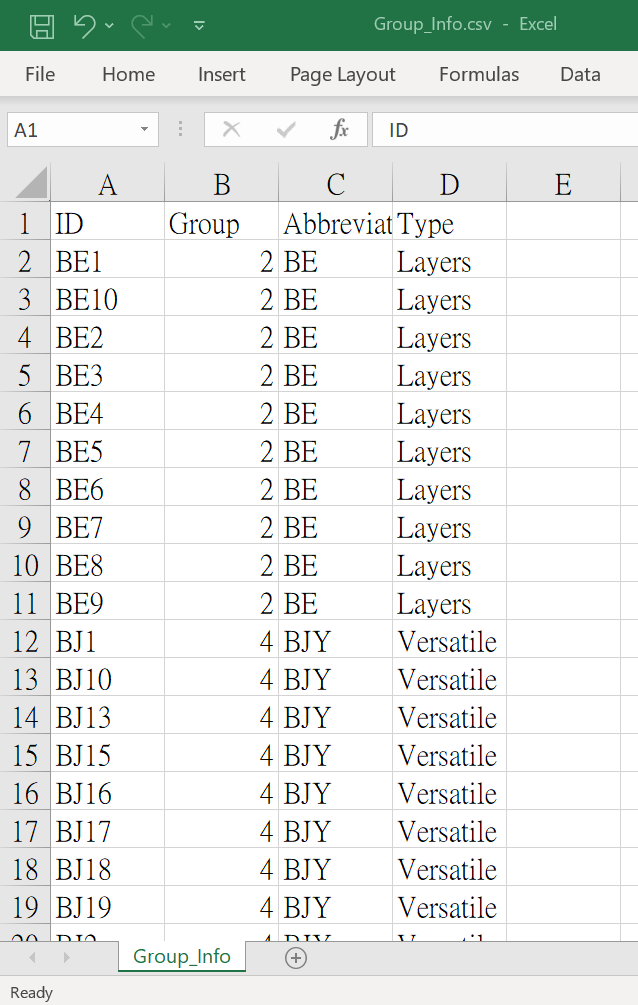
\includegraphics[width=3.64583in,height=\textheight]{images/clipboard-4028088589.png}

\paragraph*{}\label{section}
\addcontentsline{toc}{paragraph}{}

\paragraph*{\texorpdfstring{\textbf{Steps:}}{Steps:}}\label{steps-3}
\addcontentsline{toc}{paragraph}{\textbf{Steps:}}

\begin{enumerate}
\def\labelenumi{\arabic{enumi}.}
\item
  {Upload} \textbf{PCA or DAPC Object (RDS)}
\item
  {Upload} \textbf{Group and Other Info. (CSV)}
\item
  Click the {\textbf{Run Scatter Plot}} button to generate the 2D and 3D interactive scatter plots.
\item
  Customize the scatter plot and click the {\textbf{Run Scatter Plot}} button again.
\end{enumerate}

\begin{quote}
\textbf{Note}: The scatter plots are downloaded as HTML files and can be opened with browsers like Chrome or Edge.
\end{quote}

\paragraph*{Outputs:}\label{outputs-10}
\addcontentsline{toc}{paragraph}{Outputs:}

\begin{itemize}
\item
  \textbf{2D Scatter Plot (HTML)}: Two-dimensional interactive scatter plot with user-defined attributes.
\item
  \textbf{3D Scatter Plot (HTML)}: Three-dimensional interactive scatter plot with user-defined attributes.
\end{itemize}

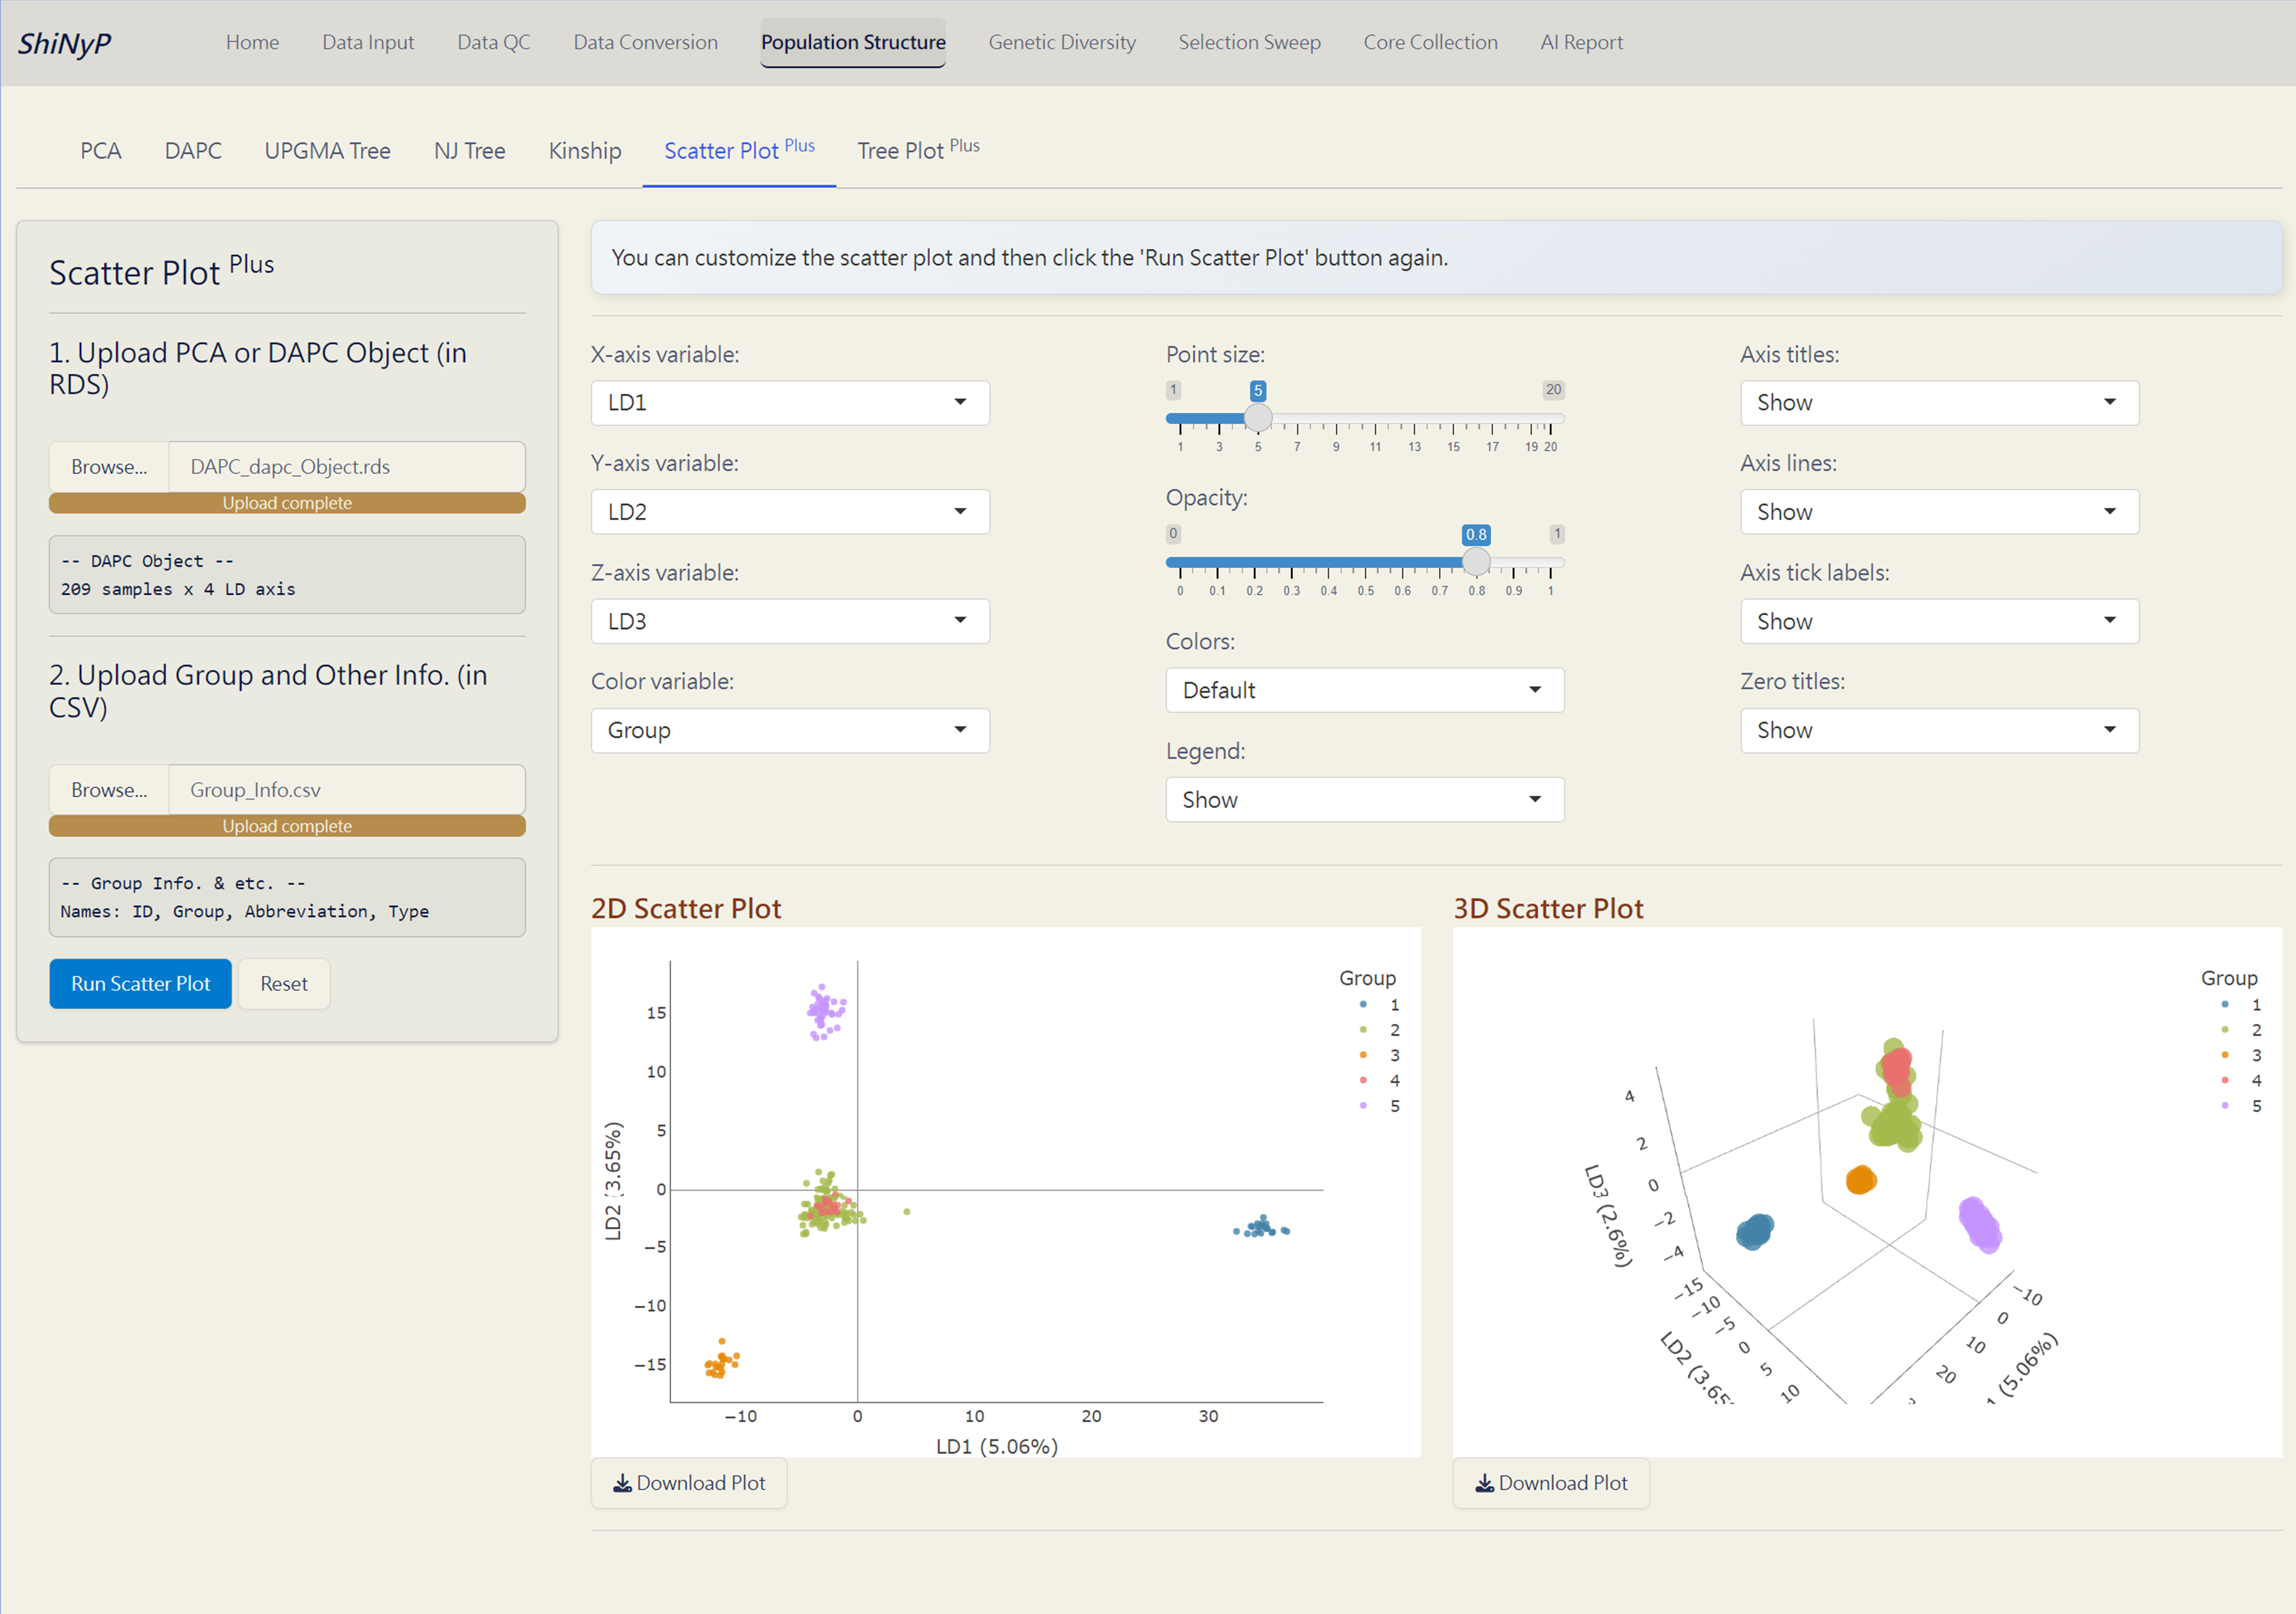
\includegraphics{images/clipboard-1525634301.png}

\emph{Scatter Plot \textsuperscript{Plus} Complete!}

\section{\texorpdfstring{Tree Plot \textsuperscript{Plus}}{Tree Plot Plus}}\label{tree-plot-plus}

Customize your phylogenetic tree plot based on the results from \ul{Population Structure}/\ul{UPGMA} or \ul{Population Structure}/\ul{NJ}.

\paragraph*{Required Files:}\label{required-files-1}
\addcontentsline{toc}{paragraph}{Required Files:}

\begin{itemize}
\tightlist
\item
  \textbf{UPGMA Object} (UPGMA\_phylo\_Object.rds file) or \textbf{NJ Object} (NJ\_phylo\_Object.rds file)
\item
  \textbf{Group and Other Info.} (modifiable from DAPC\_Group\_Info.csv)
\end{itemize}

\begin{quote}
\textbf{Note}: You can add more information about samples by adding new variables to the Group Info. file. Ensure that the sample order remains unchanged.
\end{quote}

\paragraph*{\texorpdfstring{\textbf{Steps:}}{Steps:}}\label{steps-4}
\addcontentsline{toc}{paragraph}{\textbf{Steps:}}

\begin{enumerate}
\def\labelenumi{\arabic{enumi}.}
\item
  {Upload} \textbf{UPGMA or NJ Object (RDS)}
\item
  {Upload} \textbf{Group and Other Info. (CSV)}
\item
  Click the {\textbf{Run Tree Plot}} button to generate the tree plot.
\item
  Customize the tree plot and click the {\textbf{Run Tree Plot}} button again.
\end{enumerate}

\paragraph*{Outputs:}\label{outputs-11}
\addcontentsline{toc}{paragraph}{Outputs:}

\begin{itemize}
\tightlist
\item
  \textbf{Phylogenetic Tree Plot (PDF)}: A phylogenetic tree plot with user-defined layout style and attributes.
\end{itemize}

\includegraphics{images/clipboard-2211908142.png}

\emph{Tree Plot \textsuperscript{Plus} Complete!}

\chapter{Genetic Diversity}\label{sec-genetic-diversity}

➡️ This section contains four subpages: \ul{\textbf{Diversity Parameter}}, \ul{\textbf{Circos Plot}}, \ul{\textbf{Genetic Distance}}, and \ul{\textbf{AMOVA}}, allowing you to conduct various population diversity and differentiation analyses.

\includegraphics{images/Supp. Fig. 1-5_頁面_3.jpg}

\section{Diversity Parameter}\label{diversity-parameter}

Calculate key diversity parameters for each SNP site. This approach is performed using the function from \emph{snpReady} package \citep{granato2018}.

\paragraph*{Required Datasets:}\label{required-datasets}
\addcontentsline{toc}{paragraph}{Required Datasets:}

\begin{itemize}
\tightlist
\item
  {\textbf{\texttt{data.frame}}}
\item
  \textbf{Site Info.} \textbf{(RDS)} of the current \textbf{\texttt{data.frame}}, downloadable from \ul{Data Input} or \ul{Data QC} pages.
\end{itemize}

\paragraph*{\texorpdfstring{\textbf{Steps:}}{Steps:}}\label{steps-5}
\addcontentsline{toc}{paragraph}{\textbf{Steps:}}

\begin{enumerate}
\def\labelenumi{\arabic{enumi}.}
\item
  {Upload} \textbf{Site Info.} (required).
\item
  {Upload} \textbf{Group Info.} from DAPC (optional). If uploaded, population-based parameters will be calculated.
\item
  Click the {\textbf{Run Diversity Analysis}} button to generate genetic diversity and the following downloadable files.
\end{enumerate}

\paragraph*{Outputs:}\label{outputs-12}
\addcontentsline{toc}{paragraph}{Outputs:}

\begin{itemize}
\item
  \textbf{Plot of Genetic Diversity Statistics per Site (PDF)}: A genome-wide scatter plot visualizing the user-selected parameter.
\item
  \textbf{Plot of Genetic Diversity Statistics by Group (PDF)}: A lollipop plot visualizing the user-selected parameter.
\item
  \textbf{Genetic Diversity per Site (RDS)}: Contains site information and diversity statistics, can be used as input data in the \ul{Selection Sweep}/\ul{Manhattan Plot}\textsuperscript{Plus}.
\item
  \textbf{Genetic Diversity Object (RDS)}: Contains all genetic diversity results for future use and reproducibility.
\item
  \textbf{Genetic Diversity by Group} \textbf{(CSV)}: A table showing genetic diversity based on defined group assignments.
\item
  \textbf{Fst Matrix (CSV)}: A table showing pairwise Fst based on defined group assignments.
\end{itemize}

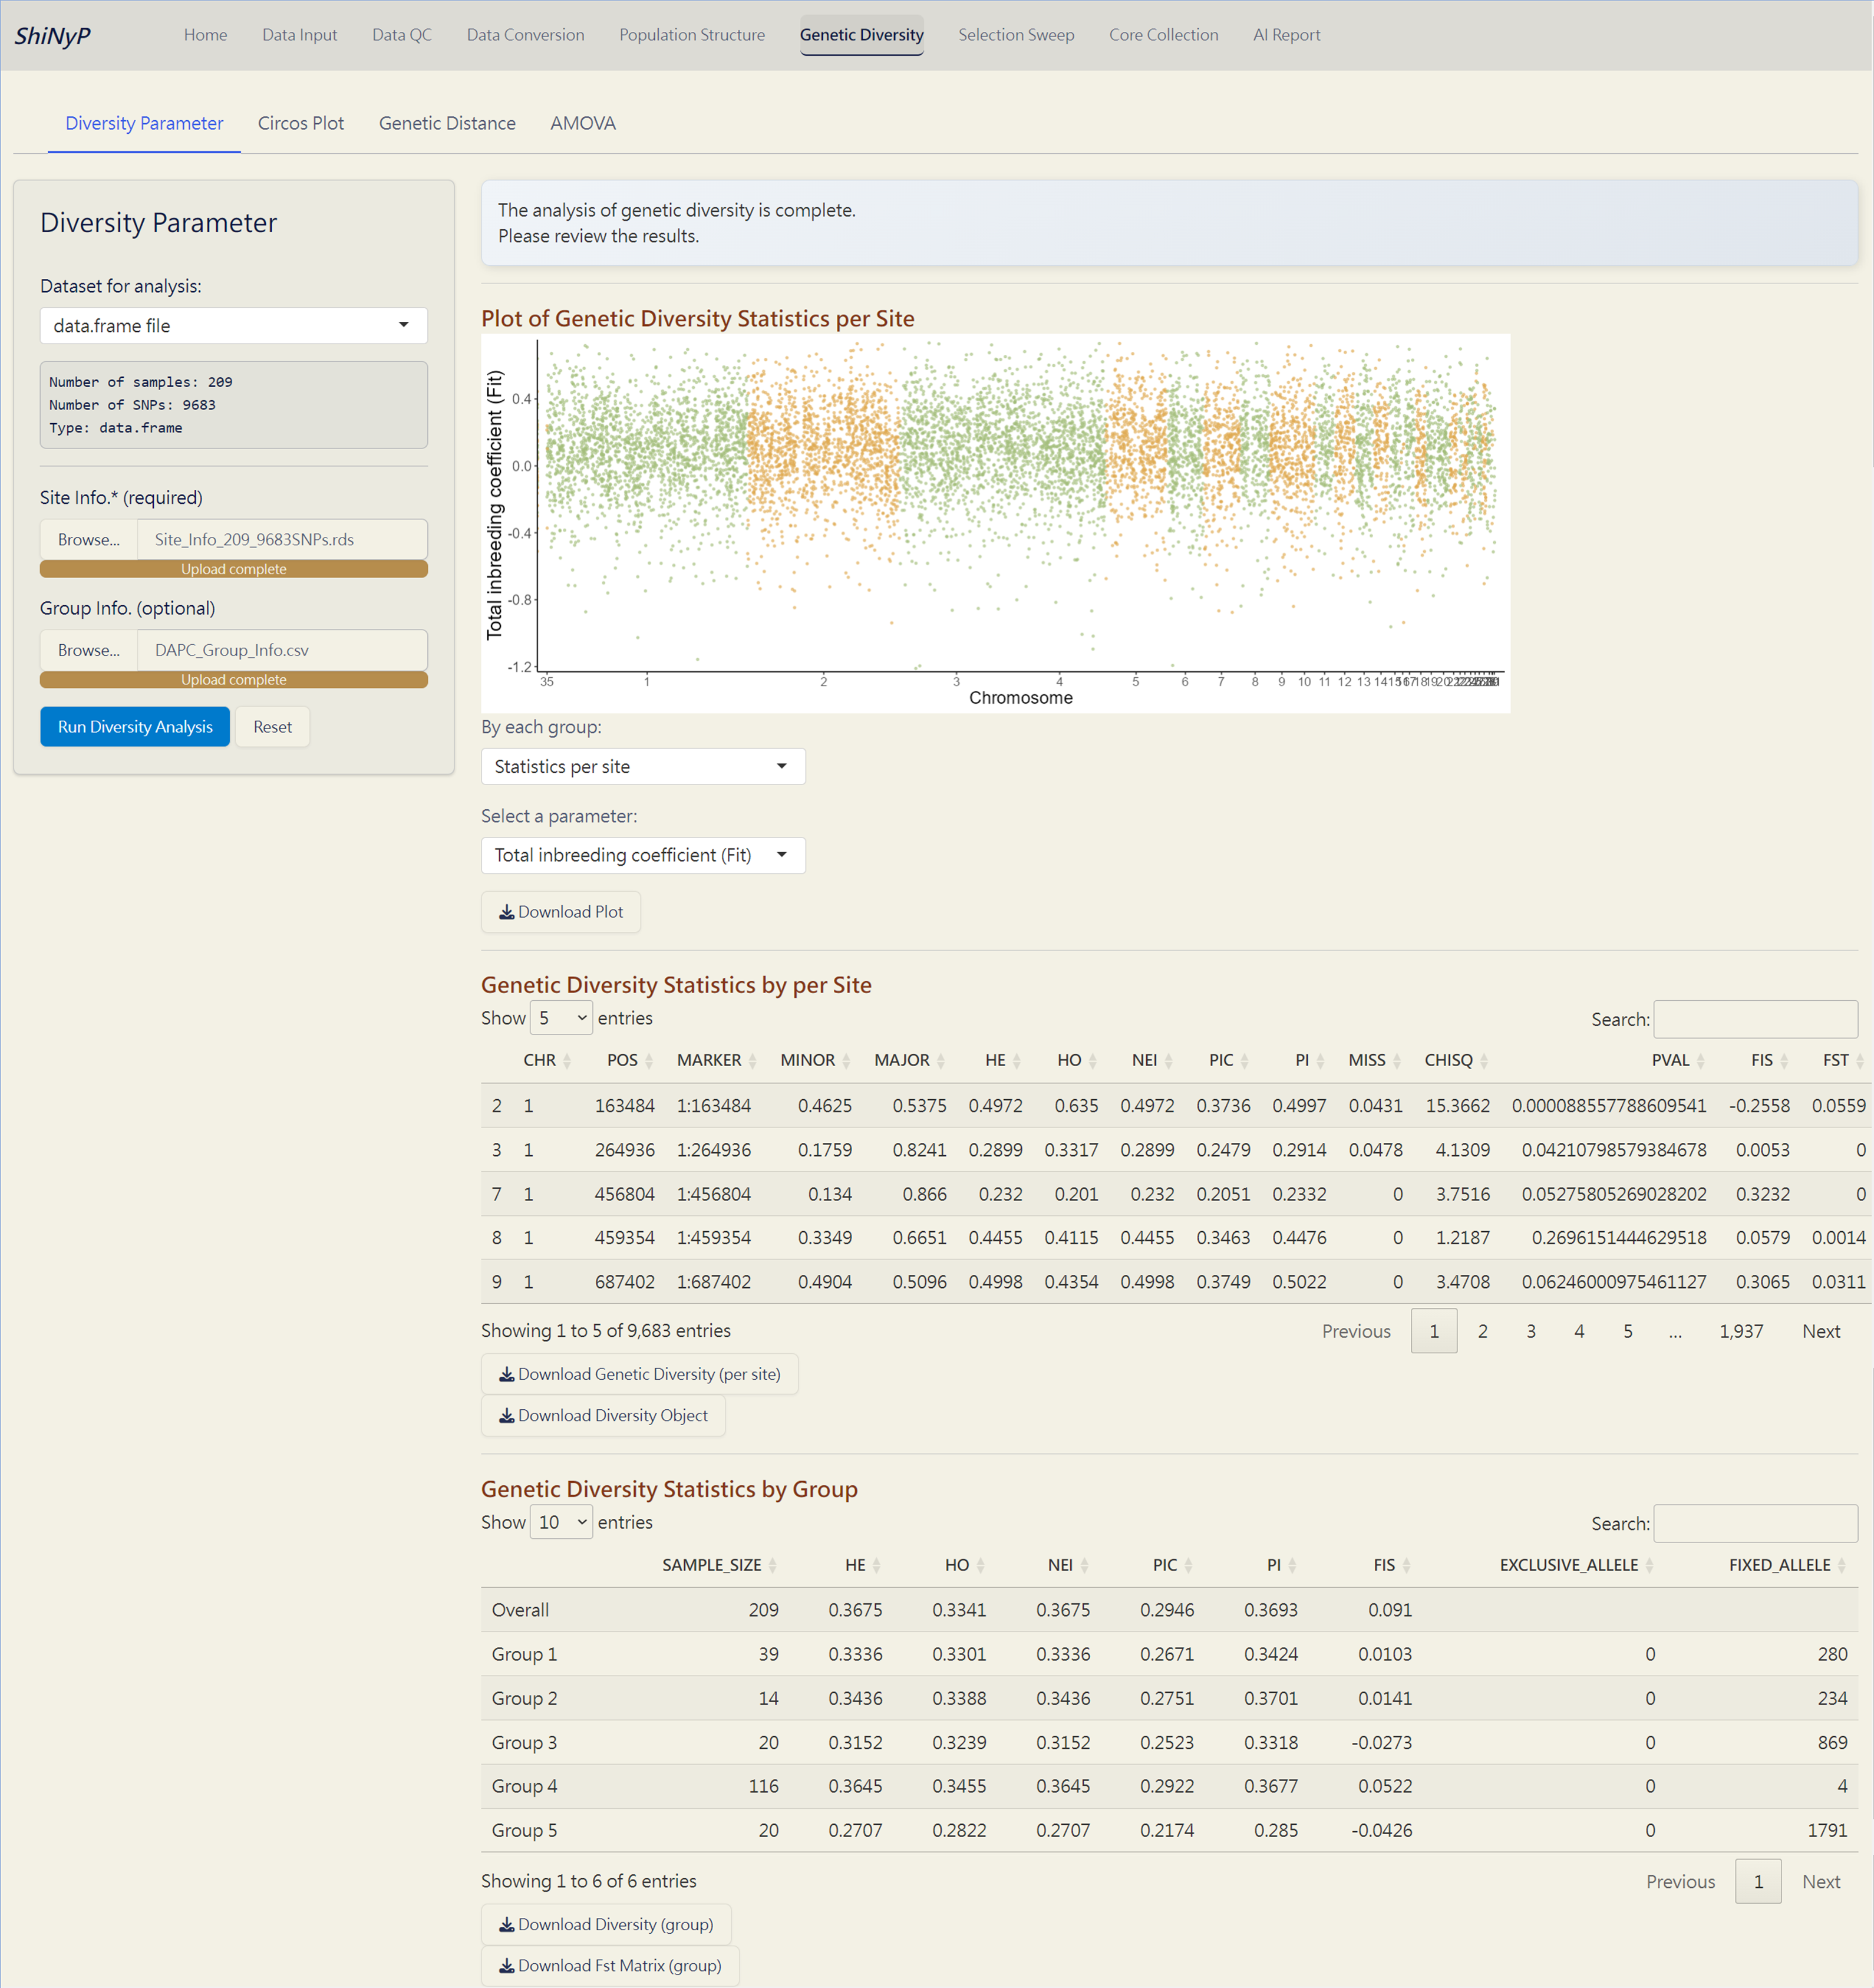
\includegraphics{images/clipboard-4215023438.png}

\emph{Diversity Analysis Complete!}

\section{Circos Plot}\label{circos-plot}

Genome-wide diversity is visualized using Circos plots generated with the \emph{circlize} package \citep{gu2014} based on results of diversity parameters in a sliding window format.

\paragraph*{Required Dataset:}\label{sec-required-dataset-chr}
\addcontentsline{toc}{paragraph}{Required Dataset:}

\begin{itemize}
\item
  Auto-import the results from the \ul{Genetic Diversity}/\ul{Diversity Parameter} subpage.
\item
  \textbf{Chromosome Info.} \textbf{(CSV)}: Reference genome information of the current study. For more details about this file, refer to \textbf{Section} \ref{snp-density} \textbf{(SNP Density)}.
\end{itemize}

\paragraph*{\texorpdfstring{\textbf{Step 1: Sliding Window}}{Step 1: Sliding Window}}\label{step-1-sliding-window}
\addcontentsline{toc}{paragraph}{\textbf{Step 1: Sliding Window}}

\begin{enumerate}
\def\labelenumi{\arabic{enumi}.}
\item
  Select parameters to generate sliding window data.
\item
  Choose window size (kb) and step size (kp).
\item
  Click the {\textbf{Run Sliding Window}} button to generate sliding window data for circos plot.
\end{enumerate}

\paragraph*{\texorpdfstring{\textbf{Step 2: Circos Plot}}{Step 2: Circos Plot}}\label{step-2-circos-plot}
\addcontentsline{toc}{paragraph}{\textbf{Step 2: Circos Plot}}

\begin{enumerate}
\def\labelenumi{\arabic{enumi}.}
\item
  {Upload} \textbf{Chromosome Info. (CSV)}.
\item
  Select a parameter for each track, and add tracks if necessary (up to a maximum of 6).
\item
  Click the {\textbf{Run Circos Plot}} button to generate the circos plot.
\end{enumerate}

\paragraph*{Outputs:}\label{outputs-13}
\addcontentsline{toc}{paragraph}{Outputs:}

\begin{itemize}
\item
  \textbf{Sliding Window Data (CSV)}: A sliding window dataset based on user-selected parameters.
\item
  \textbf{Circos Plot (PDF)}: A circos plot visualizing the user-selected parameters, with the top 1\% of each parameter colored in red.
\end{itemize}

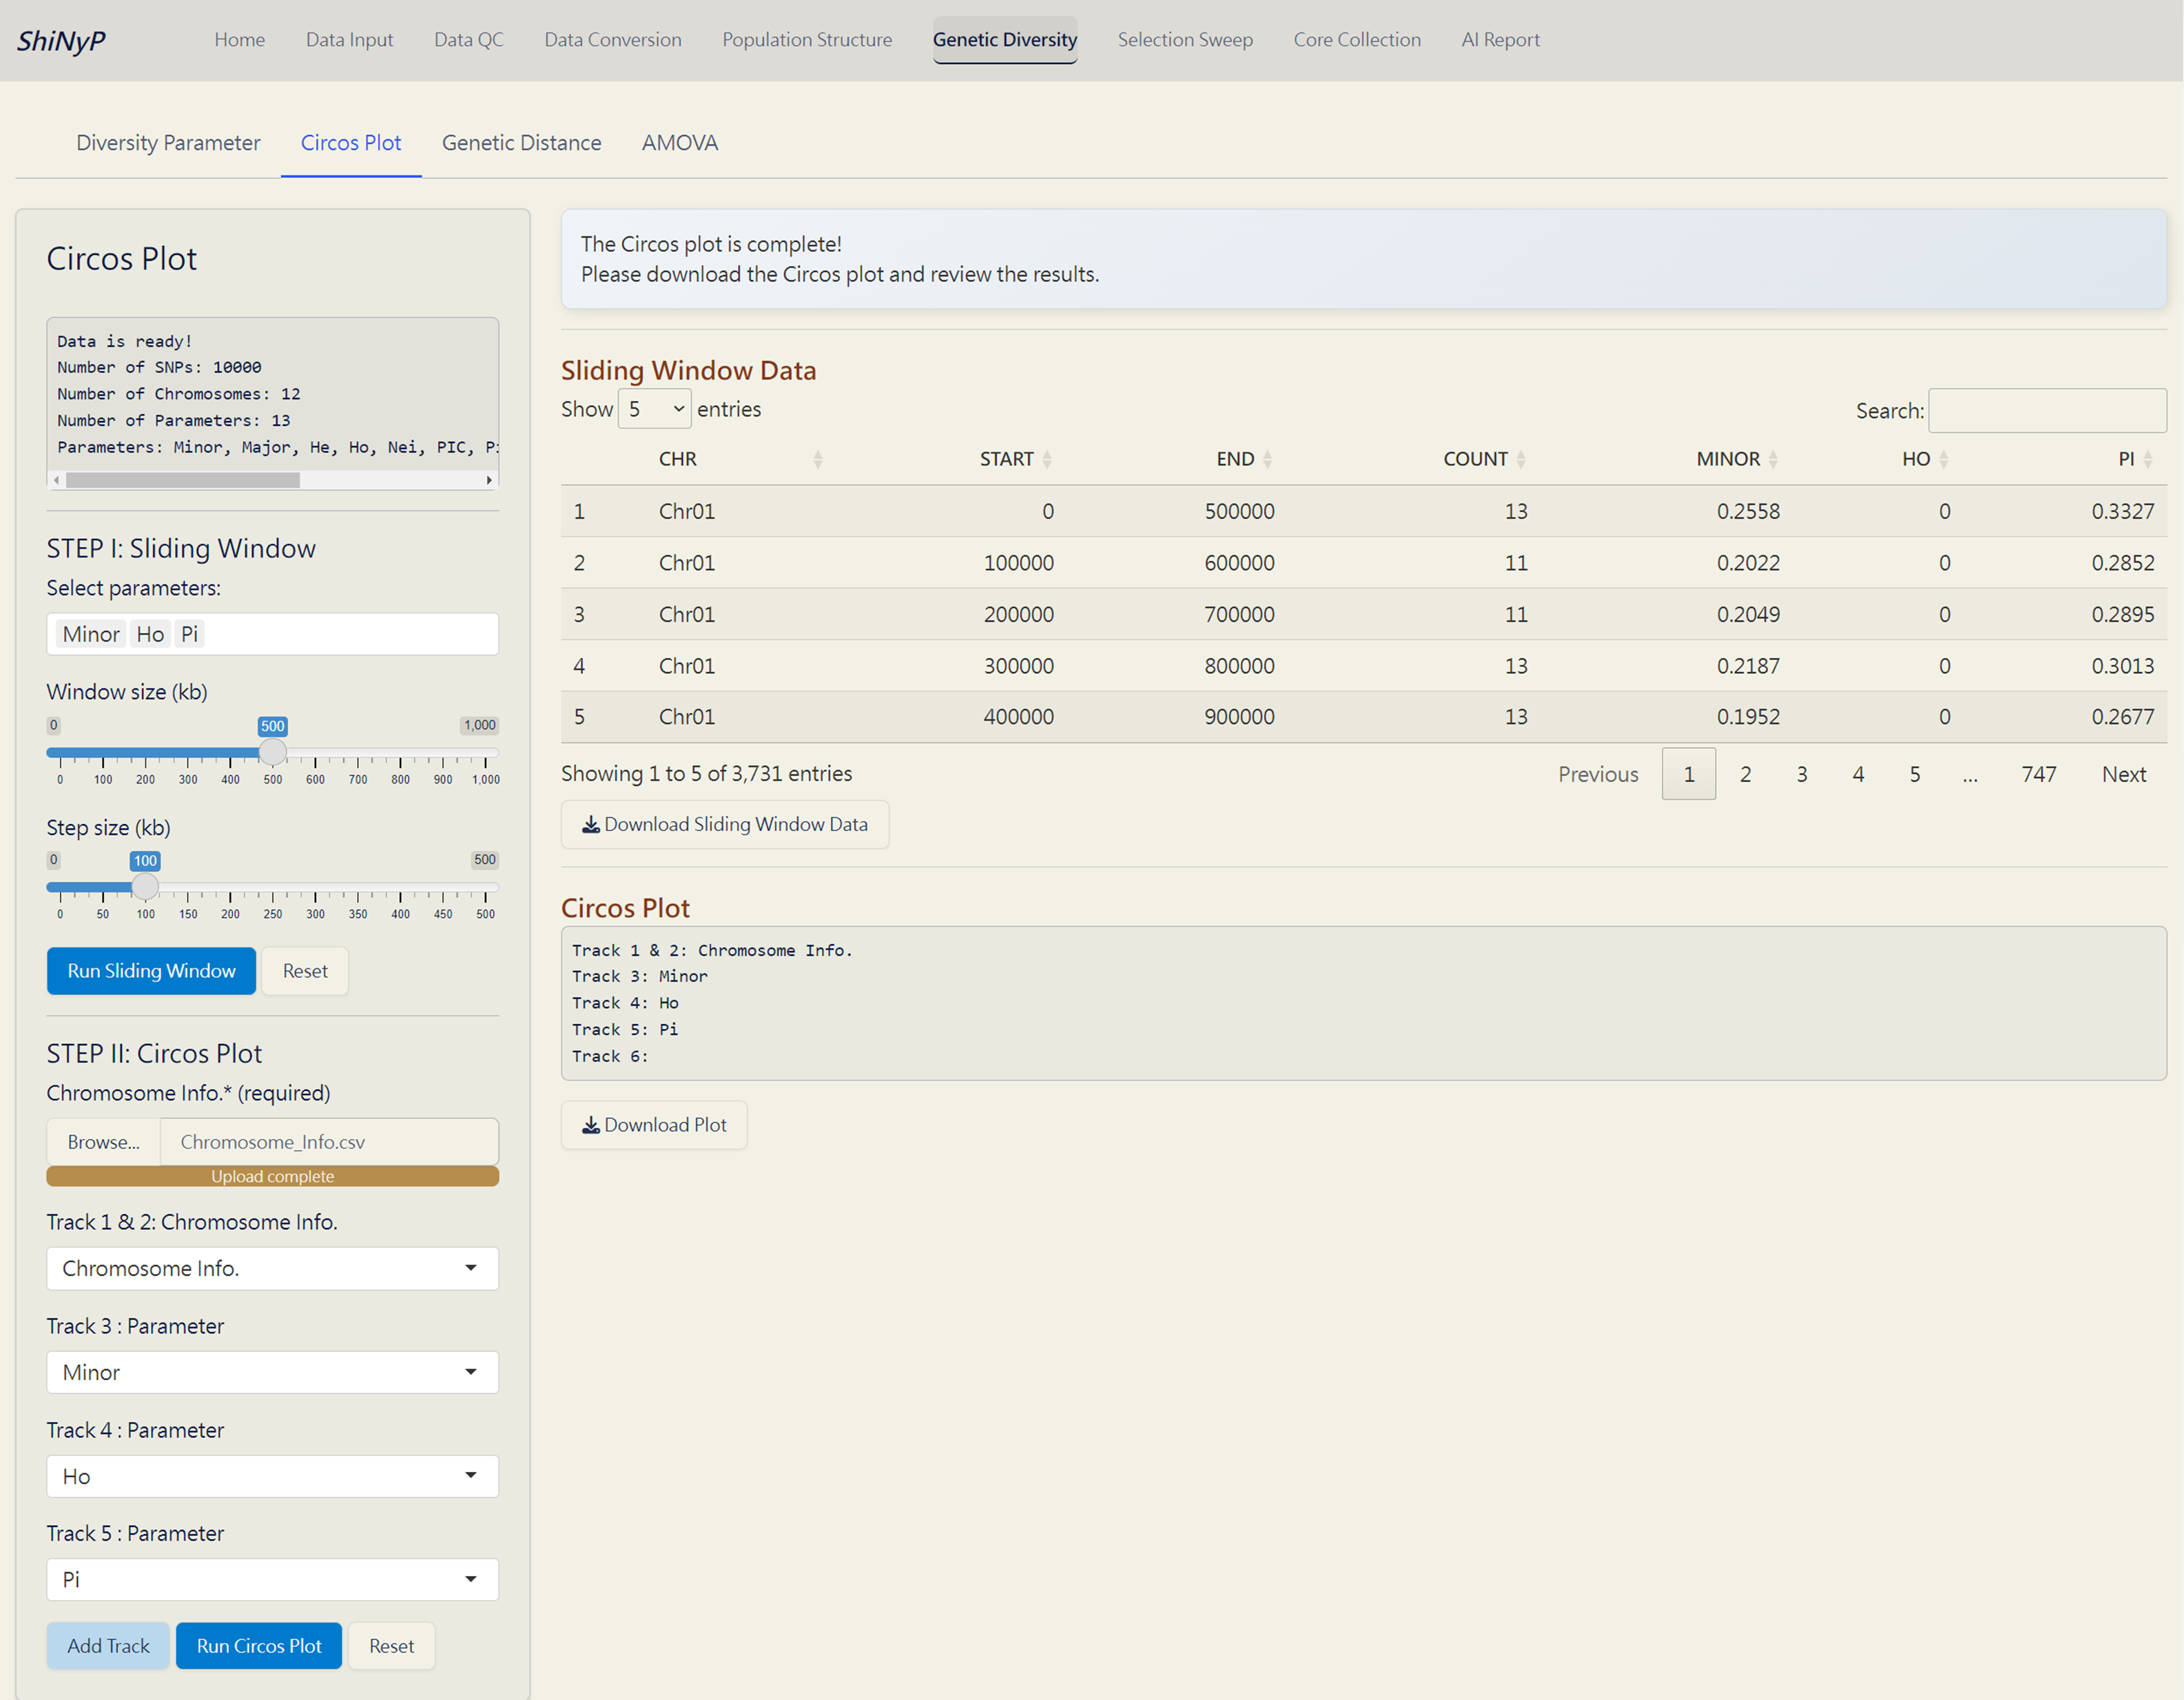
\includegraphics{images/clipboard-3157688358.png}

\emph{Circos Plot Complete!}

\section{Genetic Distance}\label{genetic-distance}

Pairwise genetic distance between populations is computed using \emph{hierfstat} package. For more information, visit https://rdrr.io/cran/hierfstat/man/genet.dist.html.

\paragraph*{Required Dataset:}\label{required-dataset-6}
\addcontentsline{toc}{paragraph}{Required Dataset:}

\begin{itemize}
\tightlist
\item
  {\textbf{\texttt{genind}}} with `Group Info.', downloadable from \ul{Data Conversion} page after you have both the {\textbf{\texttt{data.frame}}} and Group Info.
\end{itemize}

\paragraph*{\texorpdfstring{\textbf{Steps:}}{Steps:}}\label{steps-6}
\addcontentsline{toc}{paragraph}{\textbf{Steps:}}

\begin{enumerate}
\def\labelenumi{\arabic{enumi}.}
\item
  Select a method.
\item
  Click the {\textbf{Run Genetic Distance}} button to generate the pairwise genetic distance.
\end{enumerate}

\paragraph*{Outputs:}\label{outputs-14}
\addcontentsline{toc}{paragraph}{Outputs:}

\begin{itemize}
\item
  \textbf{Genetic Distance Plot (PDF)}: A plot of the pairwise genetic distance matrix based on the user-selected method.
\item
  \textbf{Genetic Distance Matrix (CSV)}: A pairwise genetic distance matrix based on the user-selected method.
\end{itemize}

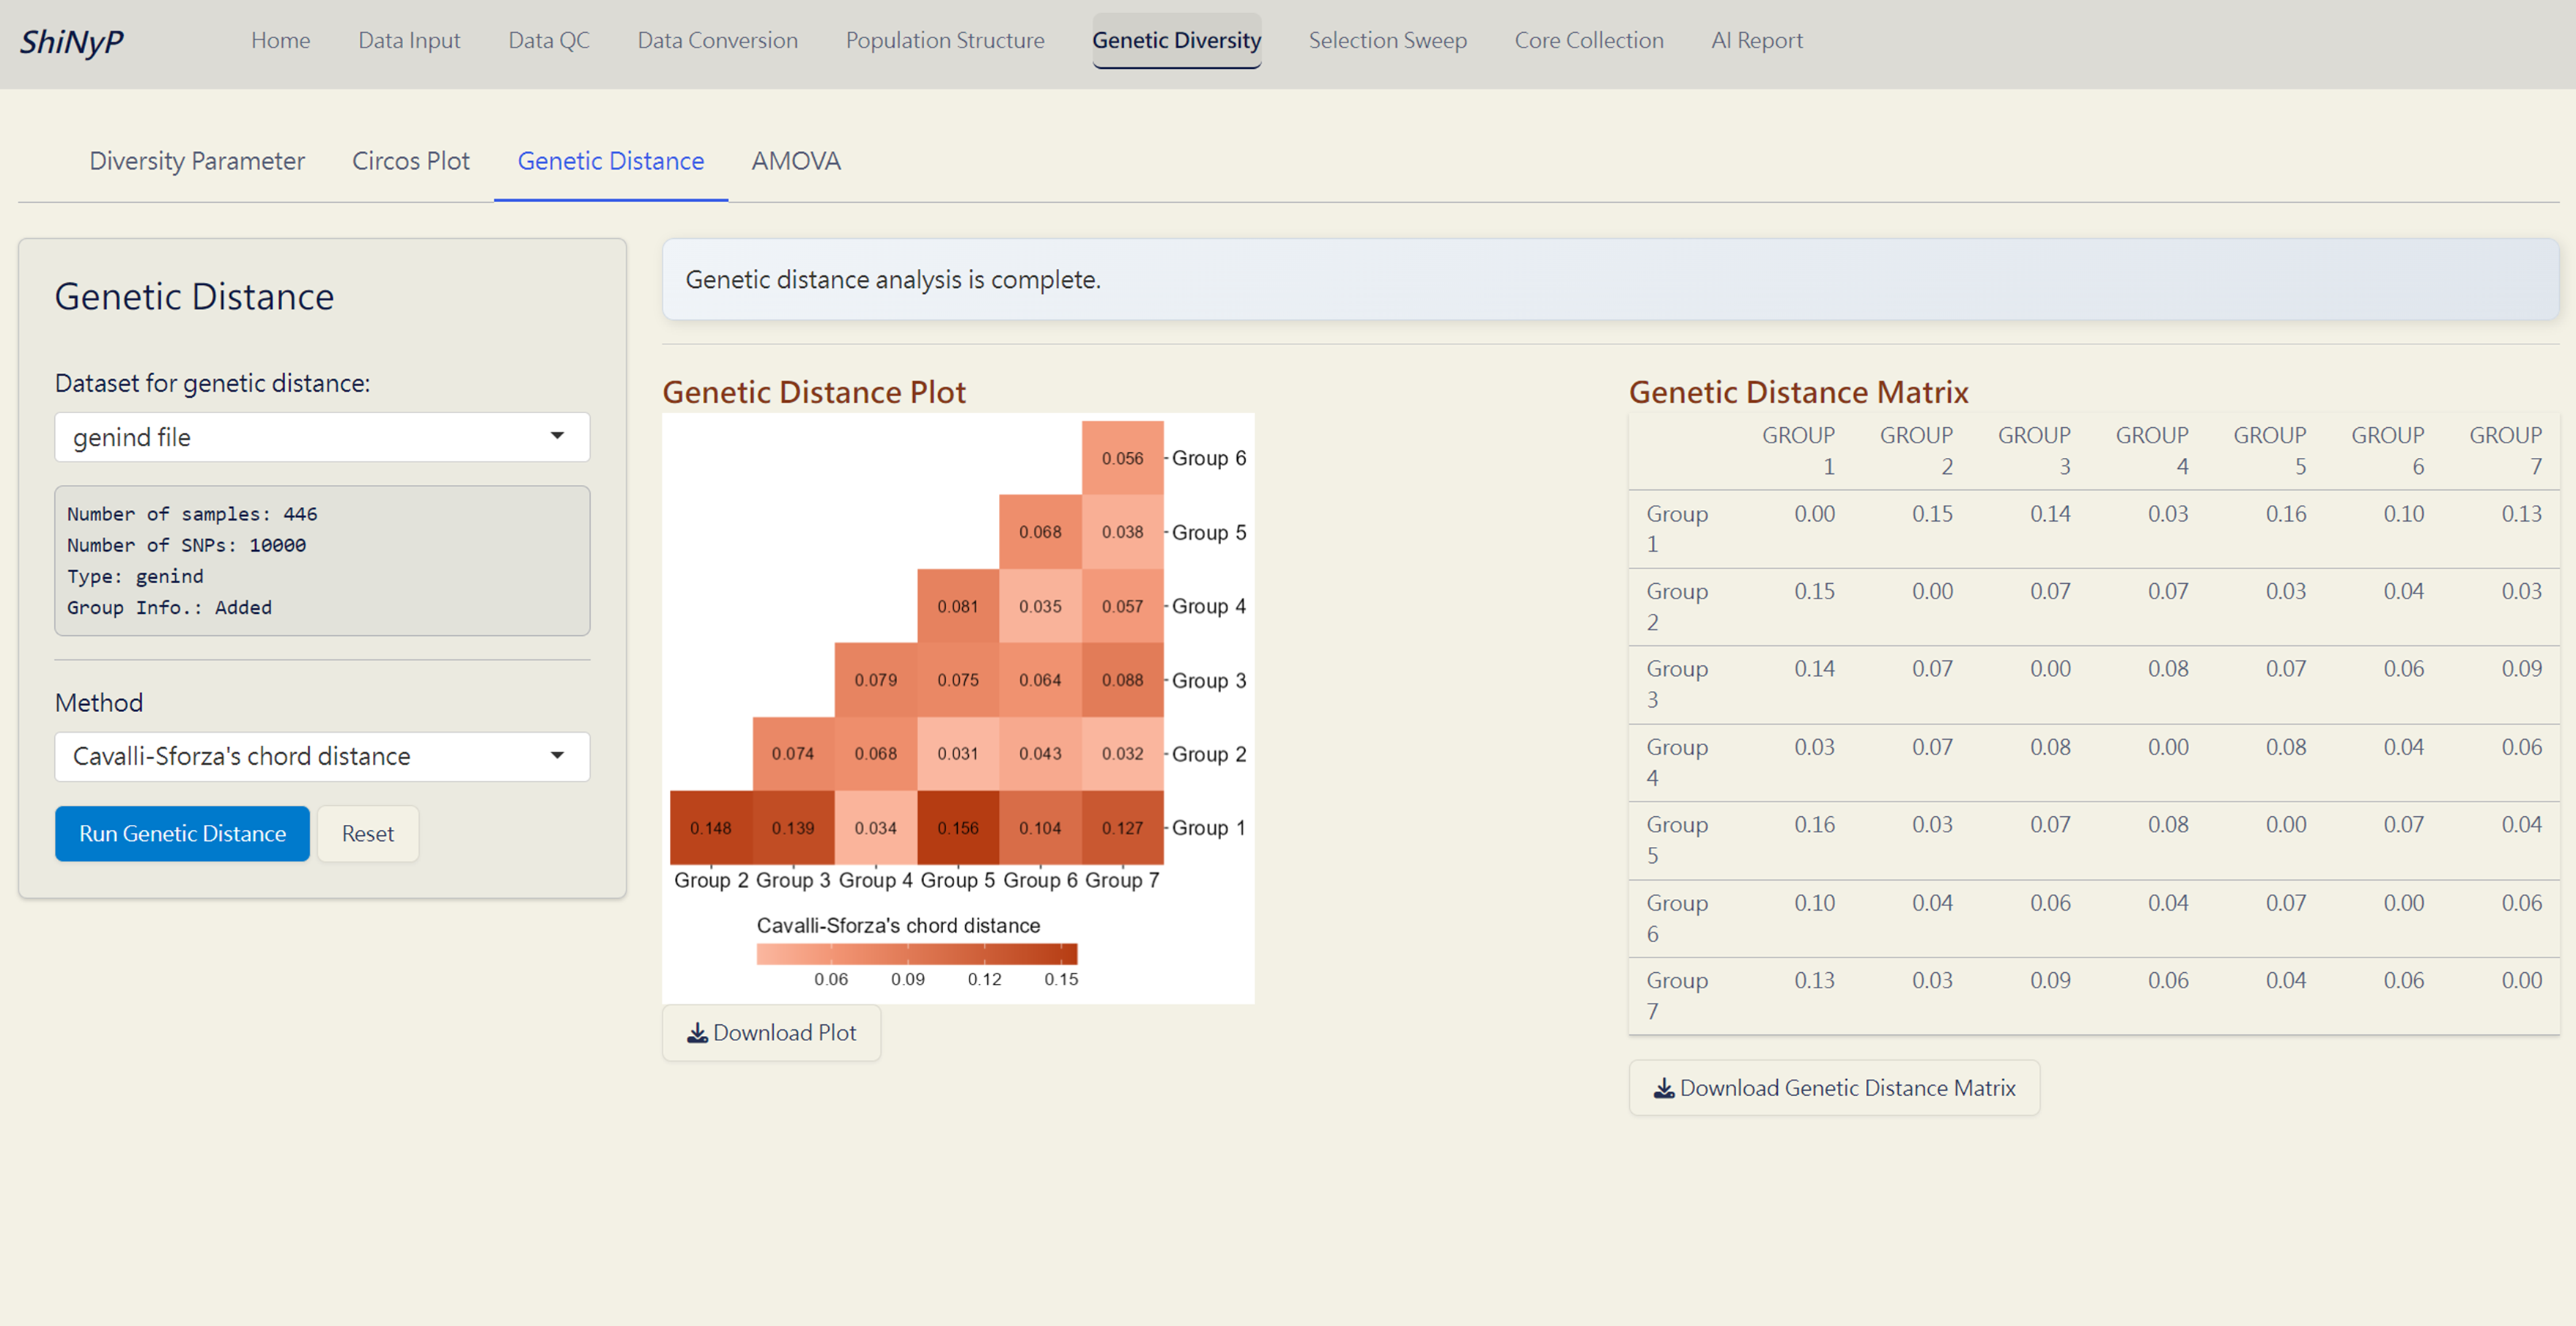
\includegraphics{images/clipboard-124406020.png}

\emph{Genetic Distance Complete!}

\section{AMOVA (Analysis of MOlecular VAriance)}\label{amova-analysis-of-molecular-variance}

A method for assessing genetic variations and relationships within and between populations \citep{excoffier1992}.This approach is performed using the function from \emph{hierfstat} and \emph{poppr} packages \citep{kamvar2014, goudet2004}.

\paragraph*{Required Dataset:}\label{required-dataset-7}
\addcontentsline{toc}{paragraph}{Required Dataset:}

\begin{itemize}
\tightlist
\item
  {\textbf{\texttt{genind}}} with `Group Info.', downloadable from \ul{Data Conversion} page after you have both the {\textbf{\texttt{data.frame}}} and Group Info.
\end{itemize}

\paragraph*{\texorpdfstring{\textbf{Step 1: Run AMOVA}}{Step 1: Run AMOVA}}\label{step-1-run-amova}
\addcontentsline{toc}{paragraph}{\textbf{Step 1: Run AMOVA}}

\begin{enumerate}
\def\labelenumi{\arabic{enumi}.}
\tightlist
\item
  Click the {\textbf{Run AMOVA}} button to partition genetic variation among and within populations.
\end{enumerate}

\paragraph*{\texorpdfstring{\textbf{Step 2: Run} Permutation Test}{Step 2: Run Permutation Test}}\label{step-2-run-permutation-test}
\addcontentsline{toc}{paragraph}{\textbf{Step 2: Run} Permutation Test}

\begin{enumerate}
\def\labelenumi{\arabic{enumi}.}
\item
  Choose the number of randomizations for the permutation test to detect the significance of three hierarchical levels. We recommend using 9, 99 (default), 199, 499, 799, or 999 permutations for more classical \emph{p}-values.
\item
  Click the {\textbf{Run Permutation Test}} button to perform the statistical test.
\end{enumerate}

\paragraph*{Outputs:}\label{outputs-15}
\addcontentsline{toc}{paragraph}{Outputs:}

\begin{itemize}
\item
  \textbf{AMOVA Variance Plot (PDF)}: A pie chart showing the explained genetic variance of population strata among defined groups.
\item
  \textbf{AMOVA Variance Test (PDF)}: A plot showing the significance test of population strata among defined groups. The histograms depict randomized strata distributions, with the black line representing genetic variance components.
\item
  \textbf{AMOVA Table (CSV)}: A table with detailed AMOVA results.
\end{itemize}

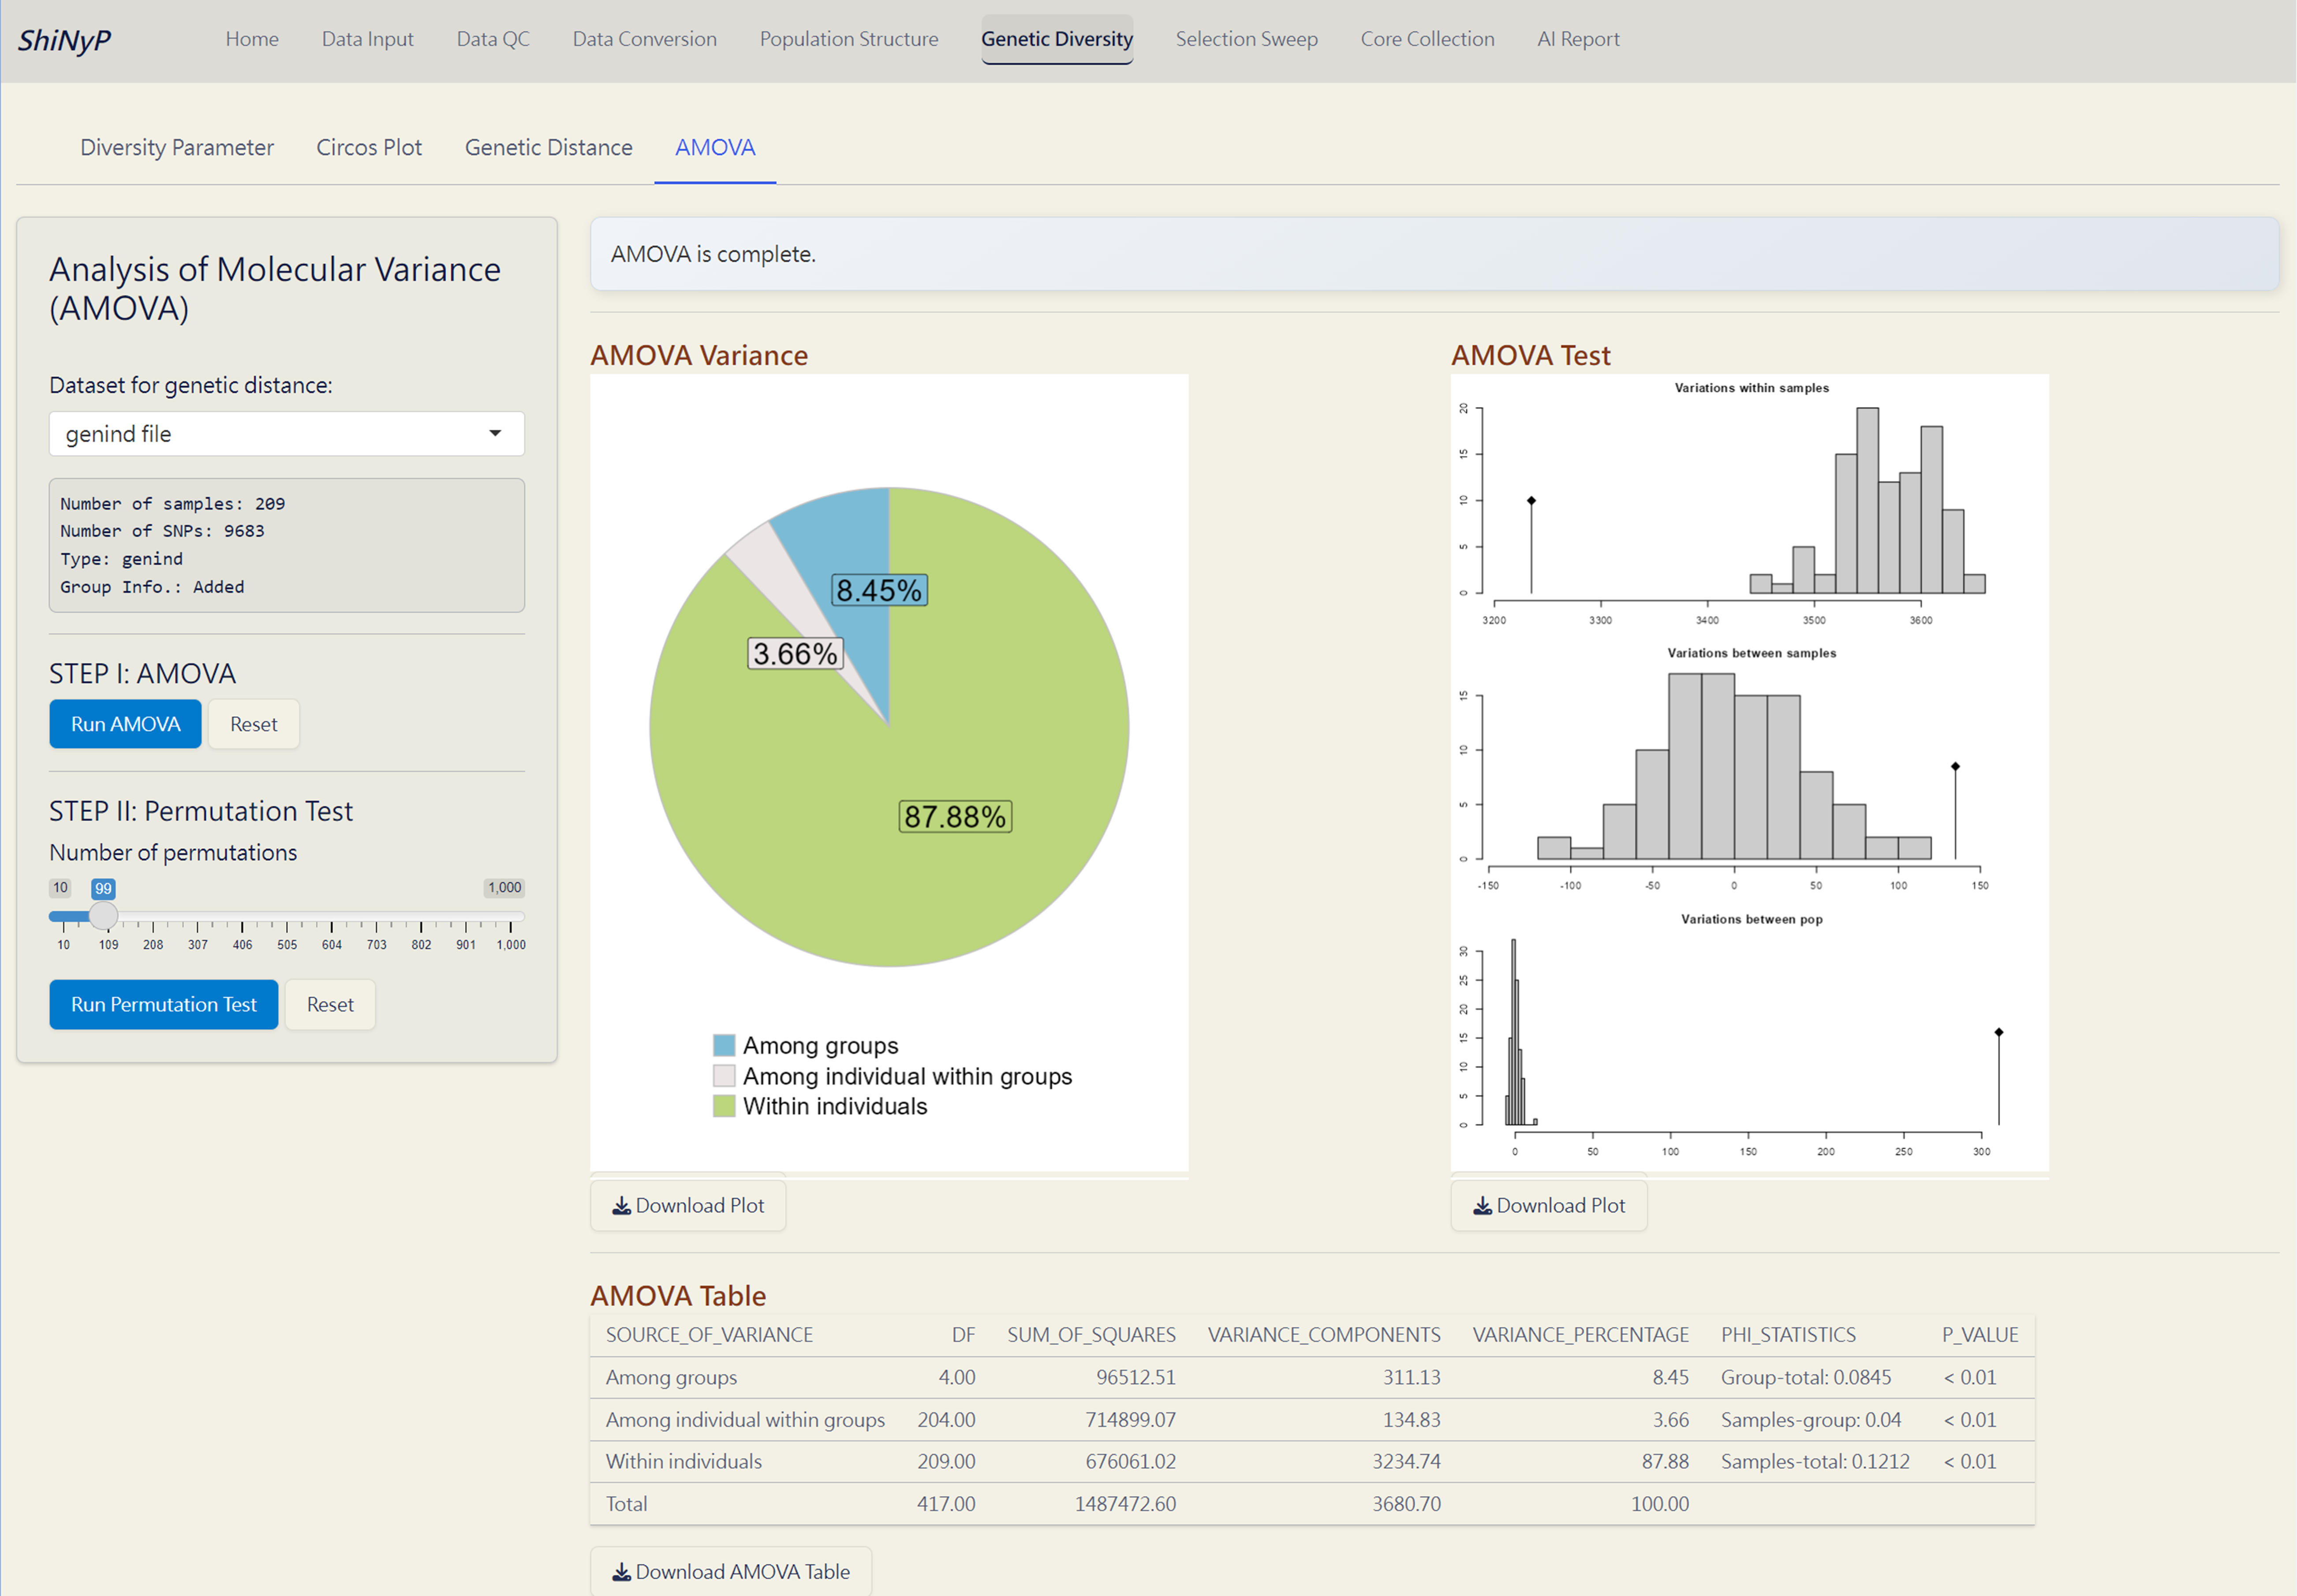
\includegraphics{images/clipboard-1689228022.png}

\emph{AMOVA Complete!}

\chapter{Selection Sweep}\label{sec-selection-sweep}

➡️ This section contains four subpages: \ul{\textbf{pcadapt}}, \ul{\textbf{OutFLANK}}, \ul{\textbf{IBS}}, and \ul{\textbf{Manhattan Plot}}\textsuperscript{\textbf{Plus}}, allowing you to detect selection signatures in different scenario and customize your plot.

\includegraphics{images/Supp. Fig. 1-5_頁面_4.jpg}

\section{pcadapt}\label{pcadapt}

A PCA-based approach identifies selective outliers relative to population structure \citep{Luu2017}.

\paragraph*{Required Datasets:}\label{required-datasets-1}
\addcontentsline{toc}{paragraph}{Required Datasets:}

\begin{itemize}
\tightlist
\item
  {\textbf{\texttt{data.frame}}}
\item
  \textbf{Site Info.} \textbf{(RDS)} of the current {\textbf{\texttt{data.frame}}}, downloadable from \ul{Data Input} or \ul{Data QC} pages.
\end{itemize}

\paragraph*{\texorpdfstring{\textbf{Steps:}}{Steps:}}\label{steps-7}
\addcontentsline{toc}{paragraph}{\textbf{Steps:}}

\begin{enumerate}
\def\labelenumi{\arabic{enumi}.}
\item
  {Upload} \textbf{Site Info.} (required).
\item
  Click {SNP Thinning} button (optional) and choose window size (number of SNPs) and r² threshold. For more information, visit https://bcm-uga.github.io/pcadapt/articles/pcadapt.html.
\item
  Click the {\textbf{Run pcadapt}} button to perform genome scan for selection.
\end{enumerate}

\paragraph*{Outputs:}\label{outputs-16}
\addcontentsline{toc}{paragraph}{Outputs:}

\begin{itemize}
\item
  \textbf{pcadapt p-value per site (RDS)}: A dataset containing p-values and adjusted p-values for each site.
\item
  \textbf{pcadapt Manhattan Plot (PDF)}: A Manhattan plot visualizing the p-values per site across the genome. Significant SNPs are highlighted in red.
\item
  \textbf{pcadapt QQ Plot (PDF)}: A QQ plot comparing the distribution of observed p-values to the expected distribution under the null hypothesis.
\item
  \textbf{pcadapt Histogram of p-values (PDF)}: A histogram showing the distribution of p-values across all sites.
\item
  \textbf{pcadapt Histogram of Test Statistics (PDF)}: A histogram showing the distribution of test statistics across all sites.
\item
  \textbf{pcadapt Significant SNPs (CSV)}: A table listing SNPs identified as significant by pcadapt, including their site info., p-values, and adjusted p-values.
\end{itemize}

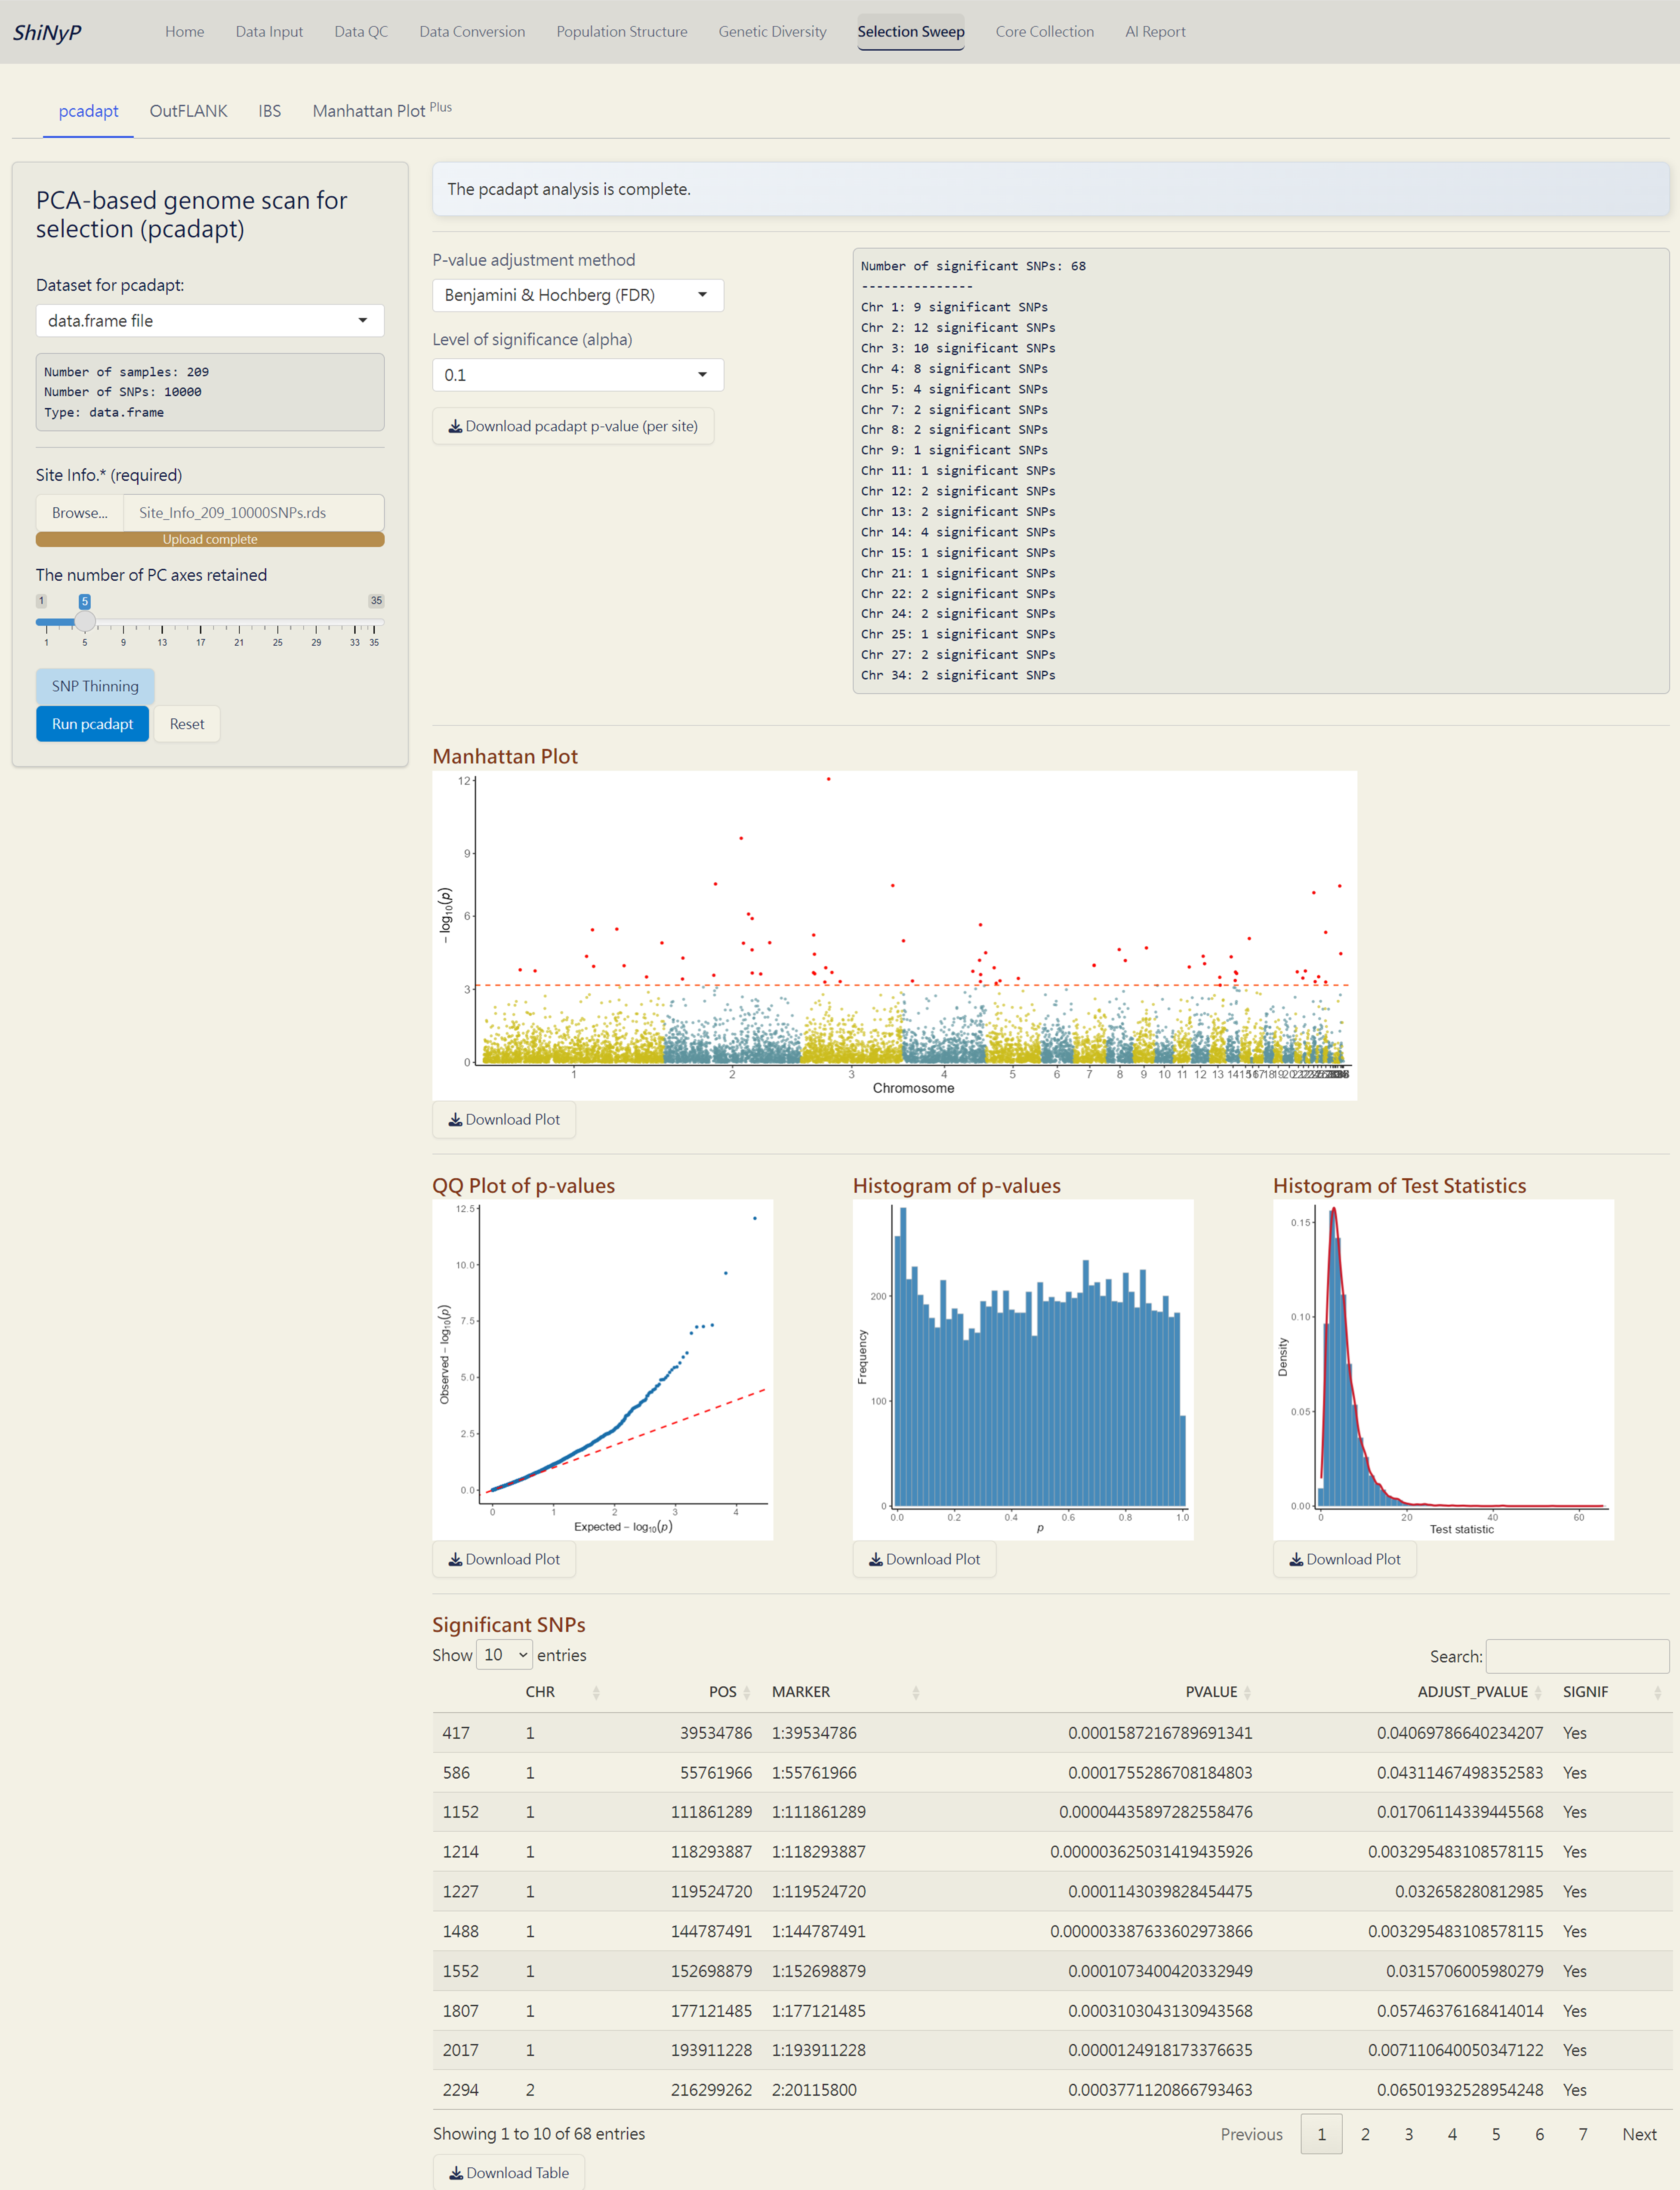
\includegraphics{images/clipboard-1914990218.png}

\emph{The pcadapt Complete!}

\section{OutFLANK}\label{outflank}

A Fst-based approach detects selection signals by comparing genetic differentiation between defined group assignments \citep{whitlock2015}. For more information, visit https://rpubs.com/lotterhos/outflank.

\paragraph*{Required Datasets:}\label{required-datasets-2}
\addcontentsline{toc}{paragraph}{Required Datasets:}

\begin{itemize}
\tightlist
\item
  {\textbf{\texttt{genind}}} with `Group Info.', downloadable from \ul{Data Conversion} page after you have both the {\textbf{\texttt{data.frame}}} and Group Info.
\item
  \textbf{Site Info.} \textbf{(RDS)} of the current {\textbf{\texttt{data.frame}}}, downloadable from \ul{Data Input} or \ul{Data QC} pages.
\end{itemize}

\paragraph*{\texorpdfstring{\textbf{Steps:}}{Steps:}}\label{steps-8}
\addcontentsline{toc}{paragraph}{\textbf{Steps:}}

\begin{enumerate}
\def\labelenumi{\arabic{enumi}.}
\item
  {Upload} \textbf{Site Info.} (required).
\item
  Click the {\textbf{Run OutFLANK}} button to perform genome scan for selection.
\end{enumerate}

\paragraph*{Outputs:}\label{outputs-17}
\addcontentsline{toc}{paragraph}{Outputs:}

\begin{itemize}
\item
  \textbf{OutFLANK} \textbf{p-value per site (RDS)}: A dataset containing p-values and adjusted p-values for each site.
\item
  \textbf{OutFLANK} \textbf{Manhattan Plot (PDF)}: A Manhattan plot visualizing the p-values per site across the genome. Significant SNPs are highlighted in red.
\item
  \textbf{OutFLANK} \textbf{QQ Plot (PDF)}: A QQ plot comparing the distribution of observed p-values to the expected distribution under the null hypothesis.
\item
  \textbf{OutFLANK} \textbf{Histogram of p-values (PDF)}: A histogram showing the distribution of p-values across all sites.
\item
  \textbf{OutFLANK} \textbf{Histogram of Fst (PDF)}: A histogram showing the distribution of Fst values across all sites.
\item
  \textbf{OutFLANK} \textbf{Significant SNPs (CSV)}: A table listing SNPs identified as significant by OutFLANK, including their site info., Fst values, and p-values.
\end{itemize}

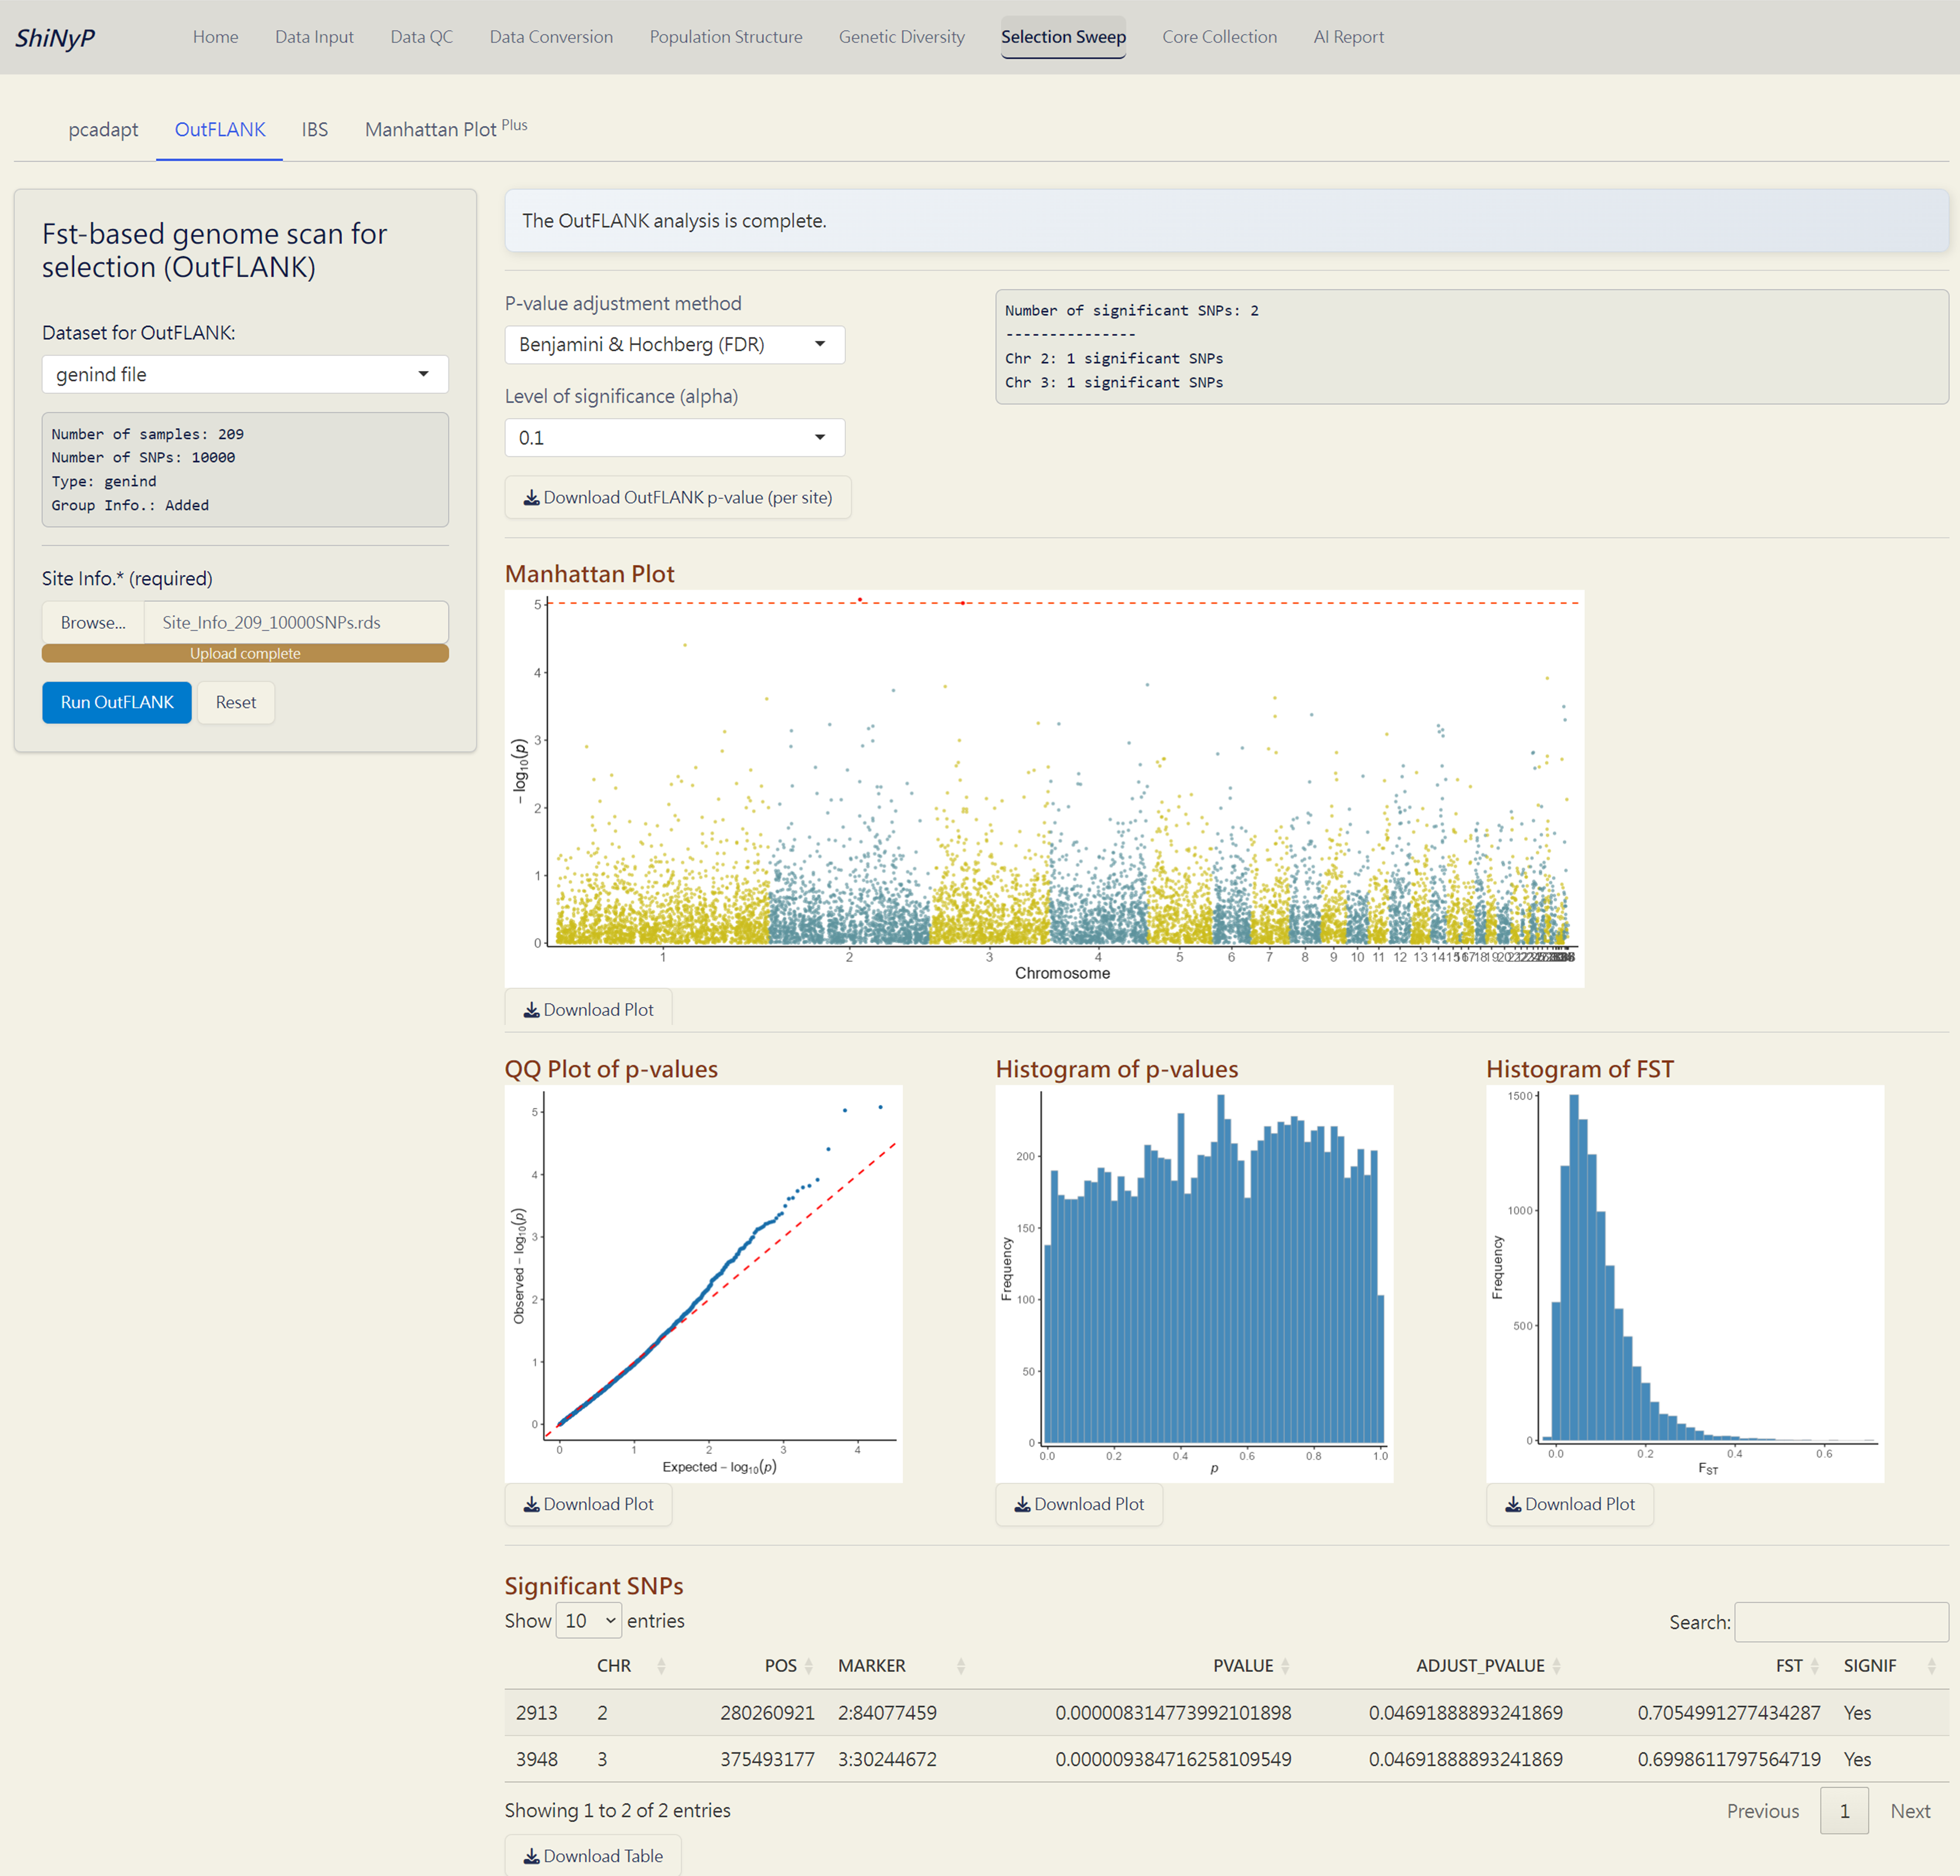
\includegraphics{images/clipboard-1859743608.png}

\emph{The OutFLANK} \emph{Complete!}

\section{IBS (Identity By State)}\label{ibs-identity-by-state}

An approach to detect differences in genomic regions between pairs of individuals, useful for identifying pedigree relationships.

\paragraph*{Required Datasets:}\label{required-datasets-3}
\addcontentsline{toc}{paragraph}{Required Datasets:}

\begin{itemize}
\tightlist
\item
  {\textbf{\texttt{data.frame}}}
\item
  \textbf{Site Info.} \textbf{(RDS)} of the current {\textbf{\texttt{data.frame}}}, downloadable from \ul{Data Input} or \ul{Data QC} pages.
\item
  \textbf{Chromosome Info.} \textbf{(CSV)}: Reference genome information of the current study. For more details about this file, refer to \textbf{Section} \ref{snp-density} \textbf{(SNP Density)}.
\end{itemize}

\paragraph*{\texorpdfstring{\textbf{Steps:}}{Steps:}}\label{steps-9}
\addcontentsline{toc}{paragraph}{\textbf{Steps:}}

\begin{enumerate}
\def\labelenumi{\arabic{enumi}.}
\item
  {Upload} \textbf{Site Info.} (required).
\item
  {Upload} \textbf{Chromosome Info.} \textbf{(CSV)} (required).
\item
  Choose the reference and comparison samples.
\item
  Select window size (kb) and step size (kp).
\item
  To remove heterozygous SNPs from the reference sample, click the {Remove heterozygous SNPs} checkbox (optional).
\item
  Click the {\textbf{Run IBS}} button to perform IBS analysis.
\end{enumerate}

\paragraph*{Outputs:}\label{outputs-18}
\addcontentsline{toc}{paragraph}{Outputs:}

\begin{itemize}
\item
  \textbf{Chromosome Ideogram (PDF)}: An ideogram visualizing the IBS results, using a gradient palette to represent the differences across chromosomes.
\item
  \textbf{Sliding Window Data (CSV)}: A sliding window dataset with IBS results, including SNP count, different SNPs, and the ratio of different SNPs per window.
\end{itemize}

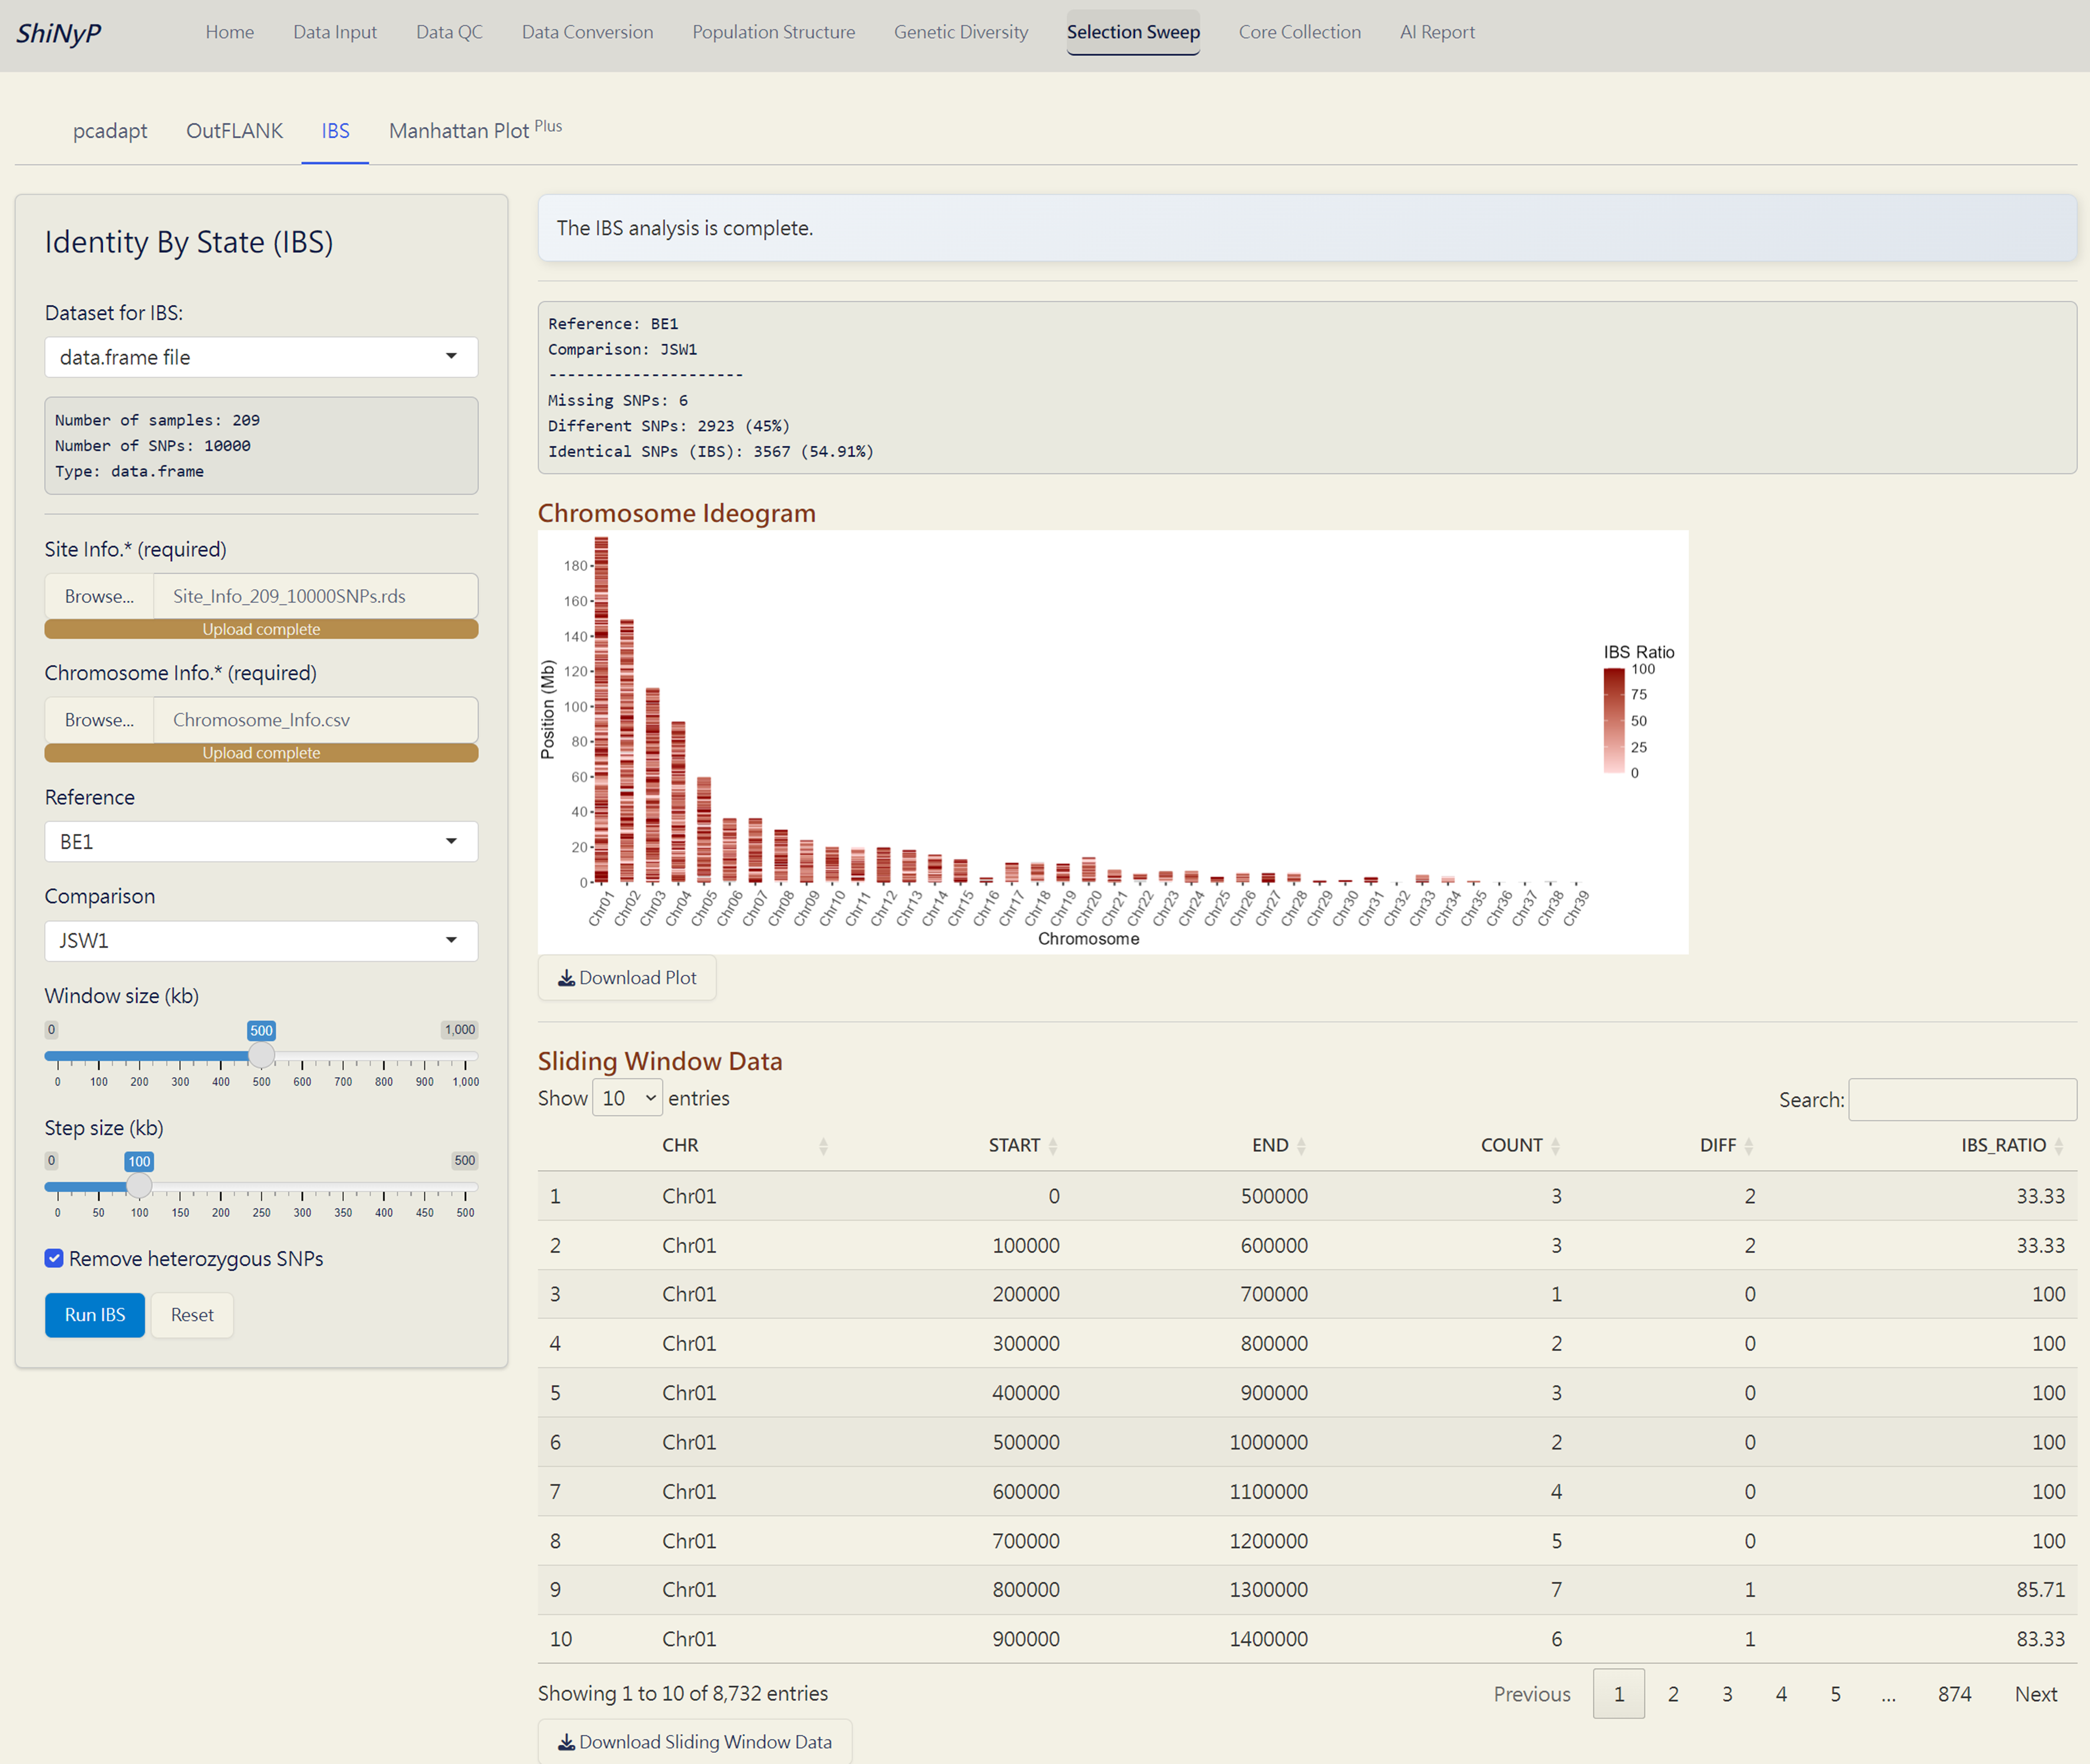
\includegraphics{images/clipboard-4086295864.png}

\emph{The IBS Complete!}

\section{\texorpdfstring{Manhattan Plot \textsuperscript{Plus}}{Manhattan Plot Plus}}\label{manhattan-plot-plus}

Customize your phylogenetic tree plot based on the results from \ul{Genetic Diversity}/\ul{Diversity Parameter}, \ul{Selection Sweep}/\ul{pcadapt}, or \ul{Selection Sweep}/\ul{OutFLANK}.

\paragraph*{Required Files:}\label{required-files-2}
\addcontentsline{toc}{paragraph}{Required Files:}

\begin{itemize}
\tightlist
\item
  \textbf{Genetic Diversity per Site} (Genetic\_Diversity\_per\_Site.rds), \textbf{pcadapt p-value per Site} (pcadapt\_p-value\_per\_site.rds), or \textbf{OutFLANK p-value per Site} (OutFLANK\_p-value\_per\_site.rds).
\item
  \textbf{Chromosome Info.} \textbf{(CSV)}: Reference genome information of the current study. For more details about this file, refer to \textbf{Section} \ref{snp-density} \textbf{(SNP Density)}.
\end{itemize}

\paragraph*{\texorpdfstring{\textbf{Steps:}}{Steps:}}\label{steps-10}
\addcontentsline{toc}{paragraph}{\textbf{Steps:}}

\begin{enumerate}
\def\labelenumi{\arabic{enumi}.}
\item
  {Upload} \textbf{genetic\_diversity/pcadapt\_pvalue/OutFLANK\_pvalue per site (RDS)}.
\item
  {Upload} \textbf{Chromosome Info. (CSV)}.
\item
  Click the {\textbf{Run Manhattan Plot}} button to generate the Manhattan plot.
\item
  Customize the Manhattan plot and click the {\textbf{Run Manhattan Plot}} button again.
\end{enumerate}

\paragraph*{Outputs:}\label{outputs-19}
\addcontentsline{toc}{paragraph}{Outputs:}

\begin{itemize}
\tightlist
\item
  \textbf{Manhattan} \textbf{Plot (PDF)}: A Manhattan plot with user-defined layout style and attributes.
\end{itemize}

\begin{quote}
\textbf{Note}: If generating a plot for p-values, make sure to use `-log10' transformation for the Y axis.
\end{quote}

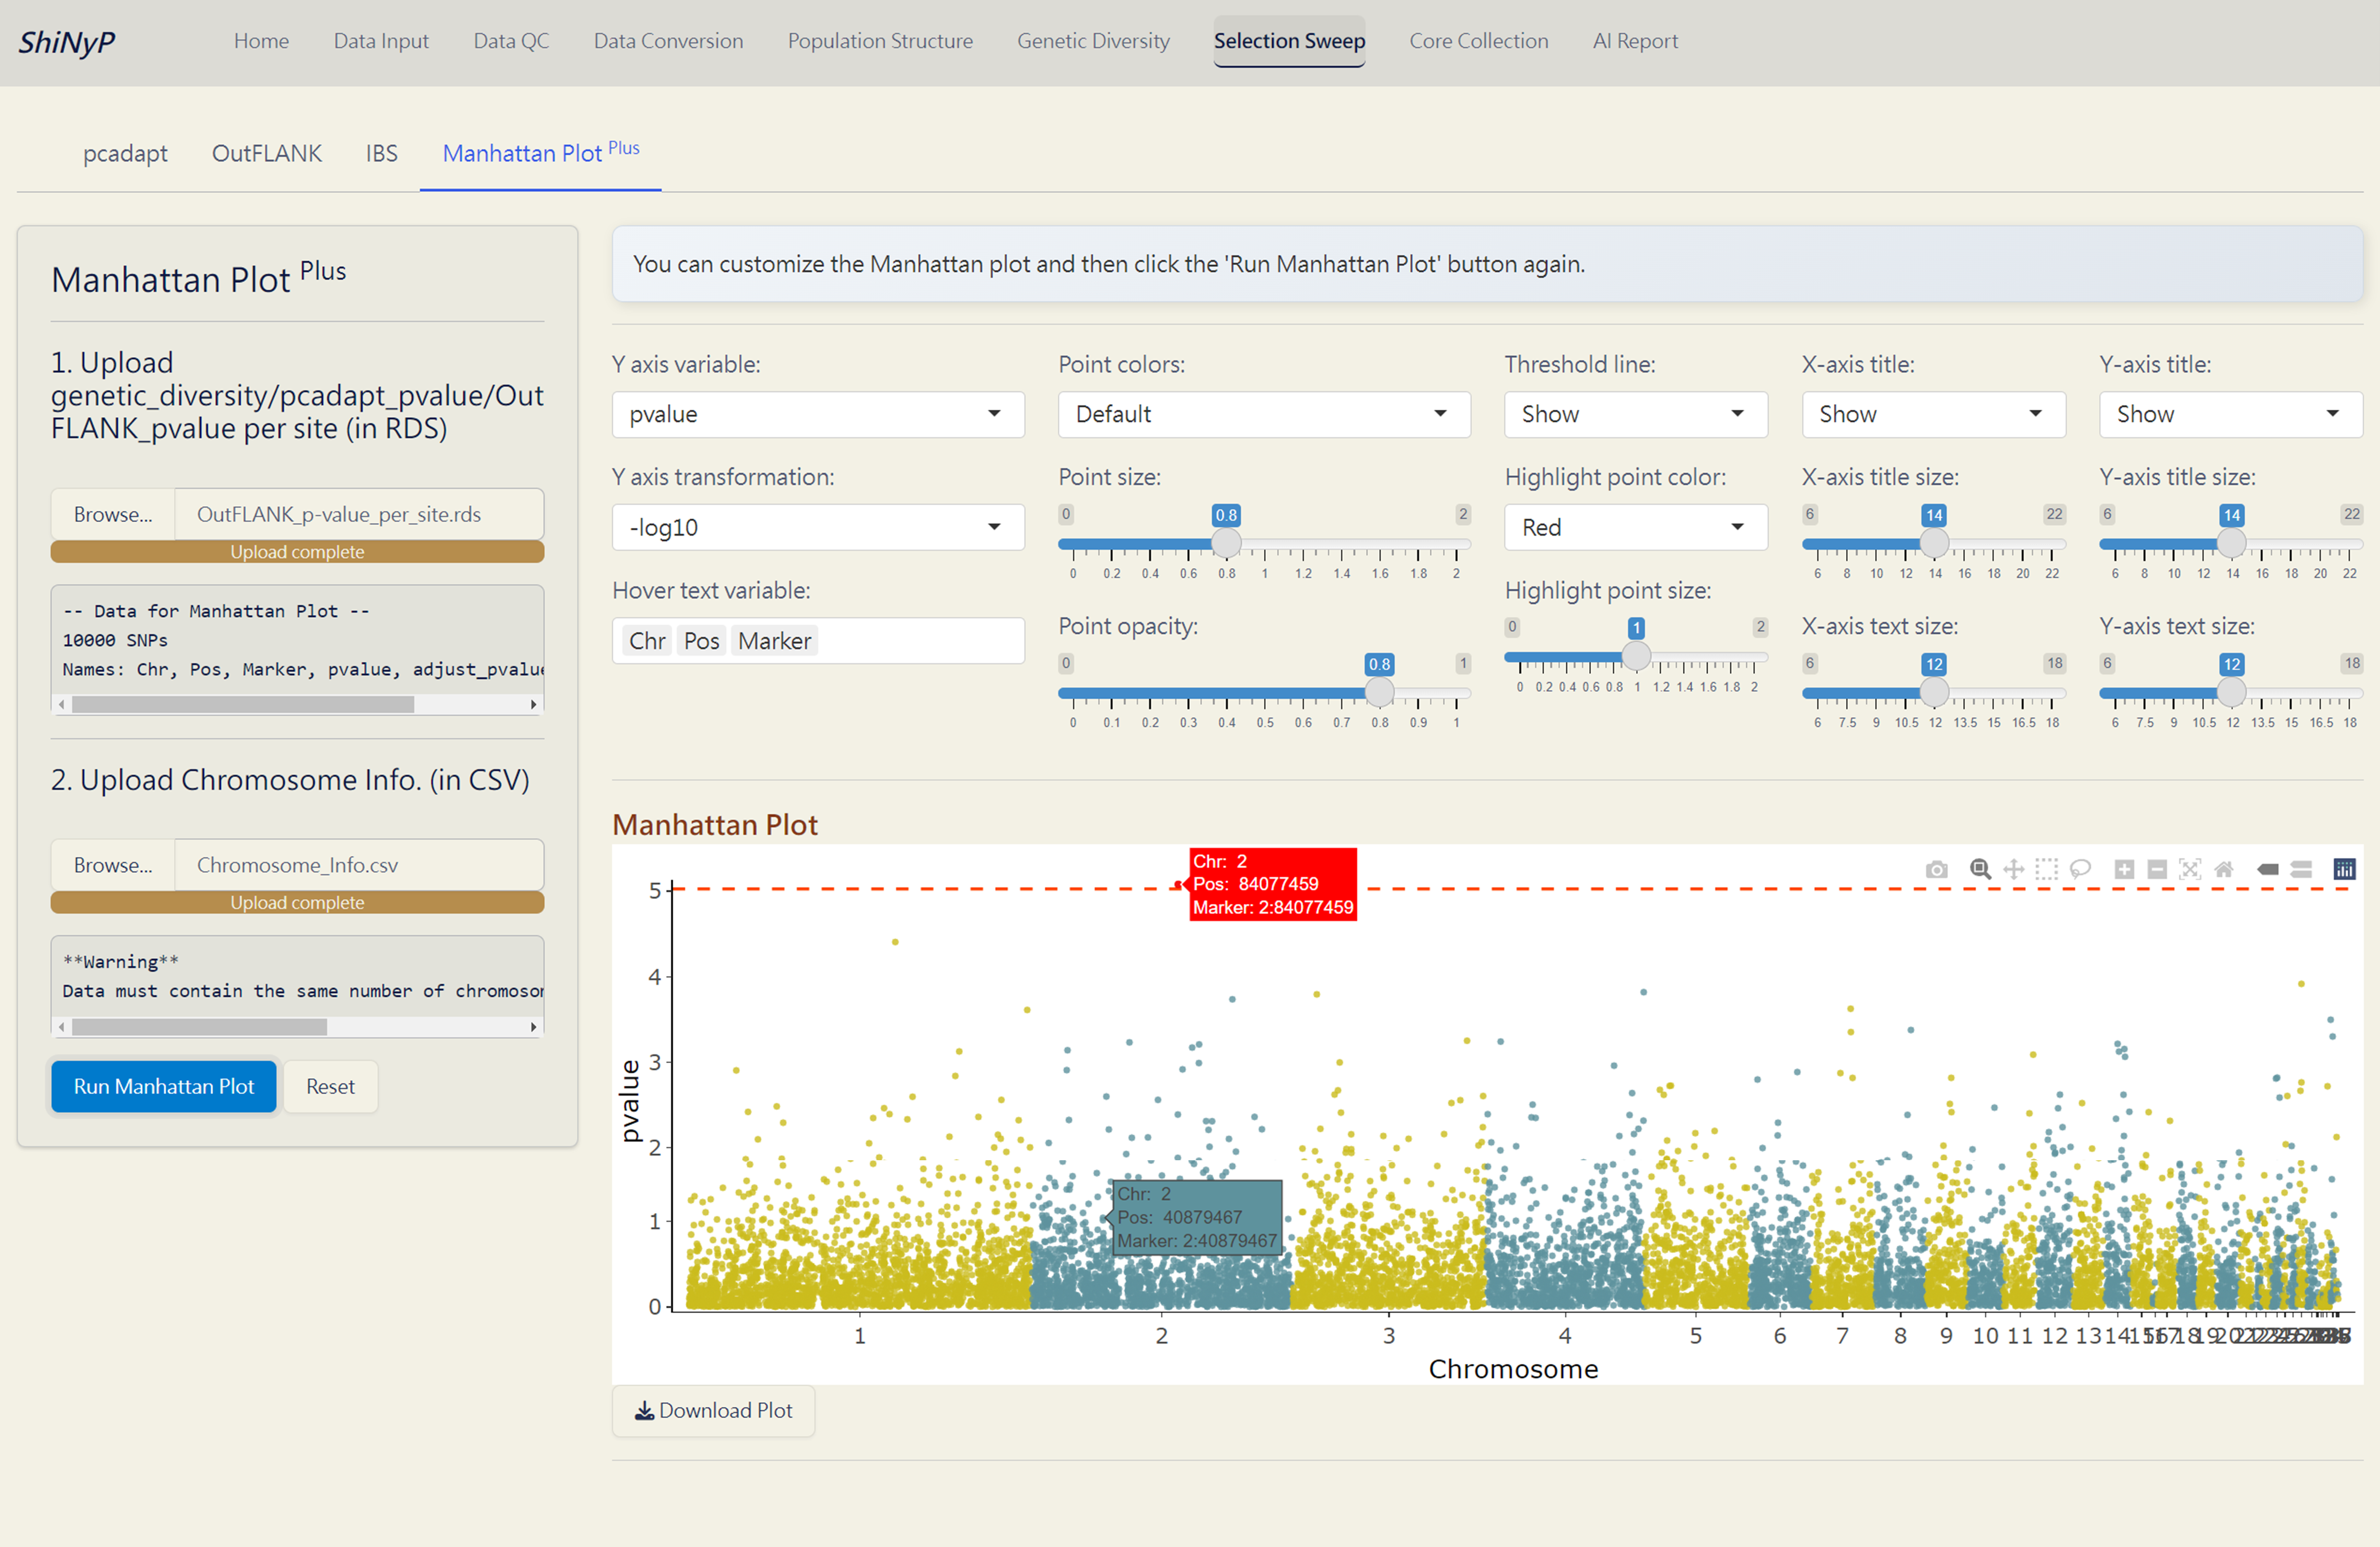
\includegraphics{images/clipboard-2598995324.png}

\emph{Manhattan} \emph{Plot \textsuperscript{Plus} Complete!}

\chapter{Core Collection}\label{sec-core-collection}

➡️ This section contains two subpages: \ul{\textbf{Core Sample Set}}, and \ul{\textbf{Core SNP Set}}, allowing you to capture the key samples and SNPs.


\includegraphics{images/Supp. Fig. 1-5_頁面_5.jpg}

\section{Core Sample Set}\label{core-sample-set}

Establish a core collection that represents the genetic variation of the entire population. This approach is modified function from GenoCore \citep{Jeong2017}.

\paragraph*{Required Datasets:}\label{required-datasets-4}
\addcontentsline{toc}{paragraph}{Required Datasets:}

\begin{itemize}
\tightlist
\item
  {\textbf{\texttt{data.frame}}}
\end{itemize}

\paragraph*{\texorpdfstring{\textbf{Steps:}}{Steps:}}\label{steps-11}
\addcontentsline{toc}{paragraph}{\textbf{Steps:}}

\begin{enumerate}
\def\labelenumi{\arabic{enumi}.}
\item
  Choose the minimum genetic coverage (\%).
\item
  Choose the genetic coverage differences between iterations.
\item
  Click the {\textbf{Run Core Sample}} button to perform core collection.
\end{enumerate}

\paragraph*{Outputs:}\label{outputs-20}
\addcontentsline{toc}{paragraph}{Outputs:}

\begin{itemize}
\item
  \textbf{Core Sample Coverage Data (CSV)}: A table listing the coverage (\%) of each iteration and coverage differences between iterations.
\item
  \textbf{Core Sample Set (RDS)}: A {\textbf{\texttt{data.frame}}} of core samples and their genotypic information.
\item
  \textbf{Core Sample Info. (CSV)}: A table listing whether each sample is included in the core collection or not, and can be used as input data in the \ul{Population Structure}/\ul{PCA} subpage.
\item
  \textbf{Coverage Plot of Core Sample Set (PDF)}: Visualizes the sample coverage by each iteration.
\end{itemize}

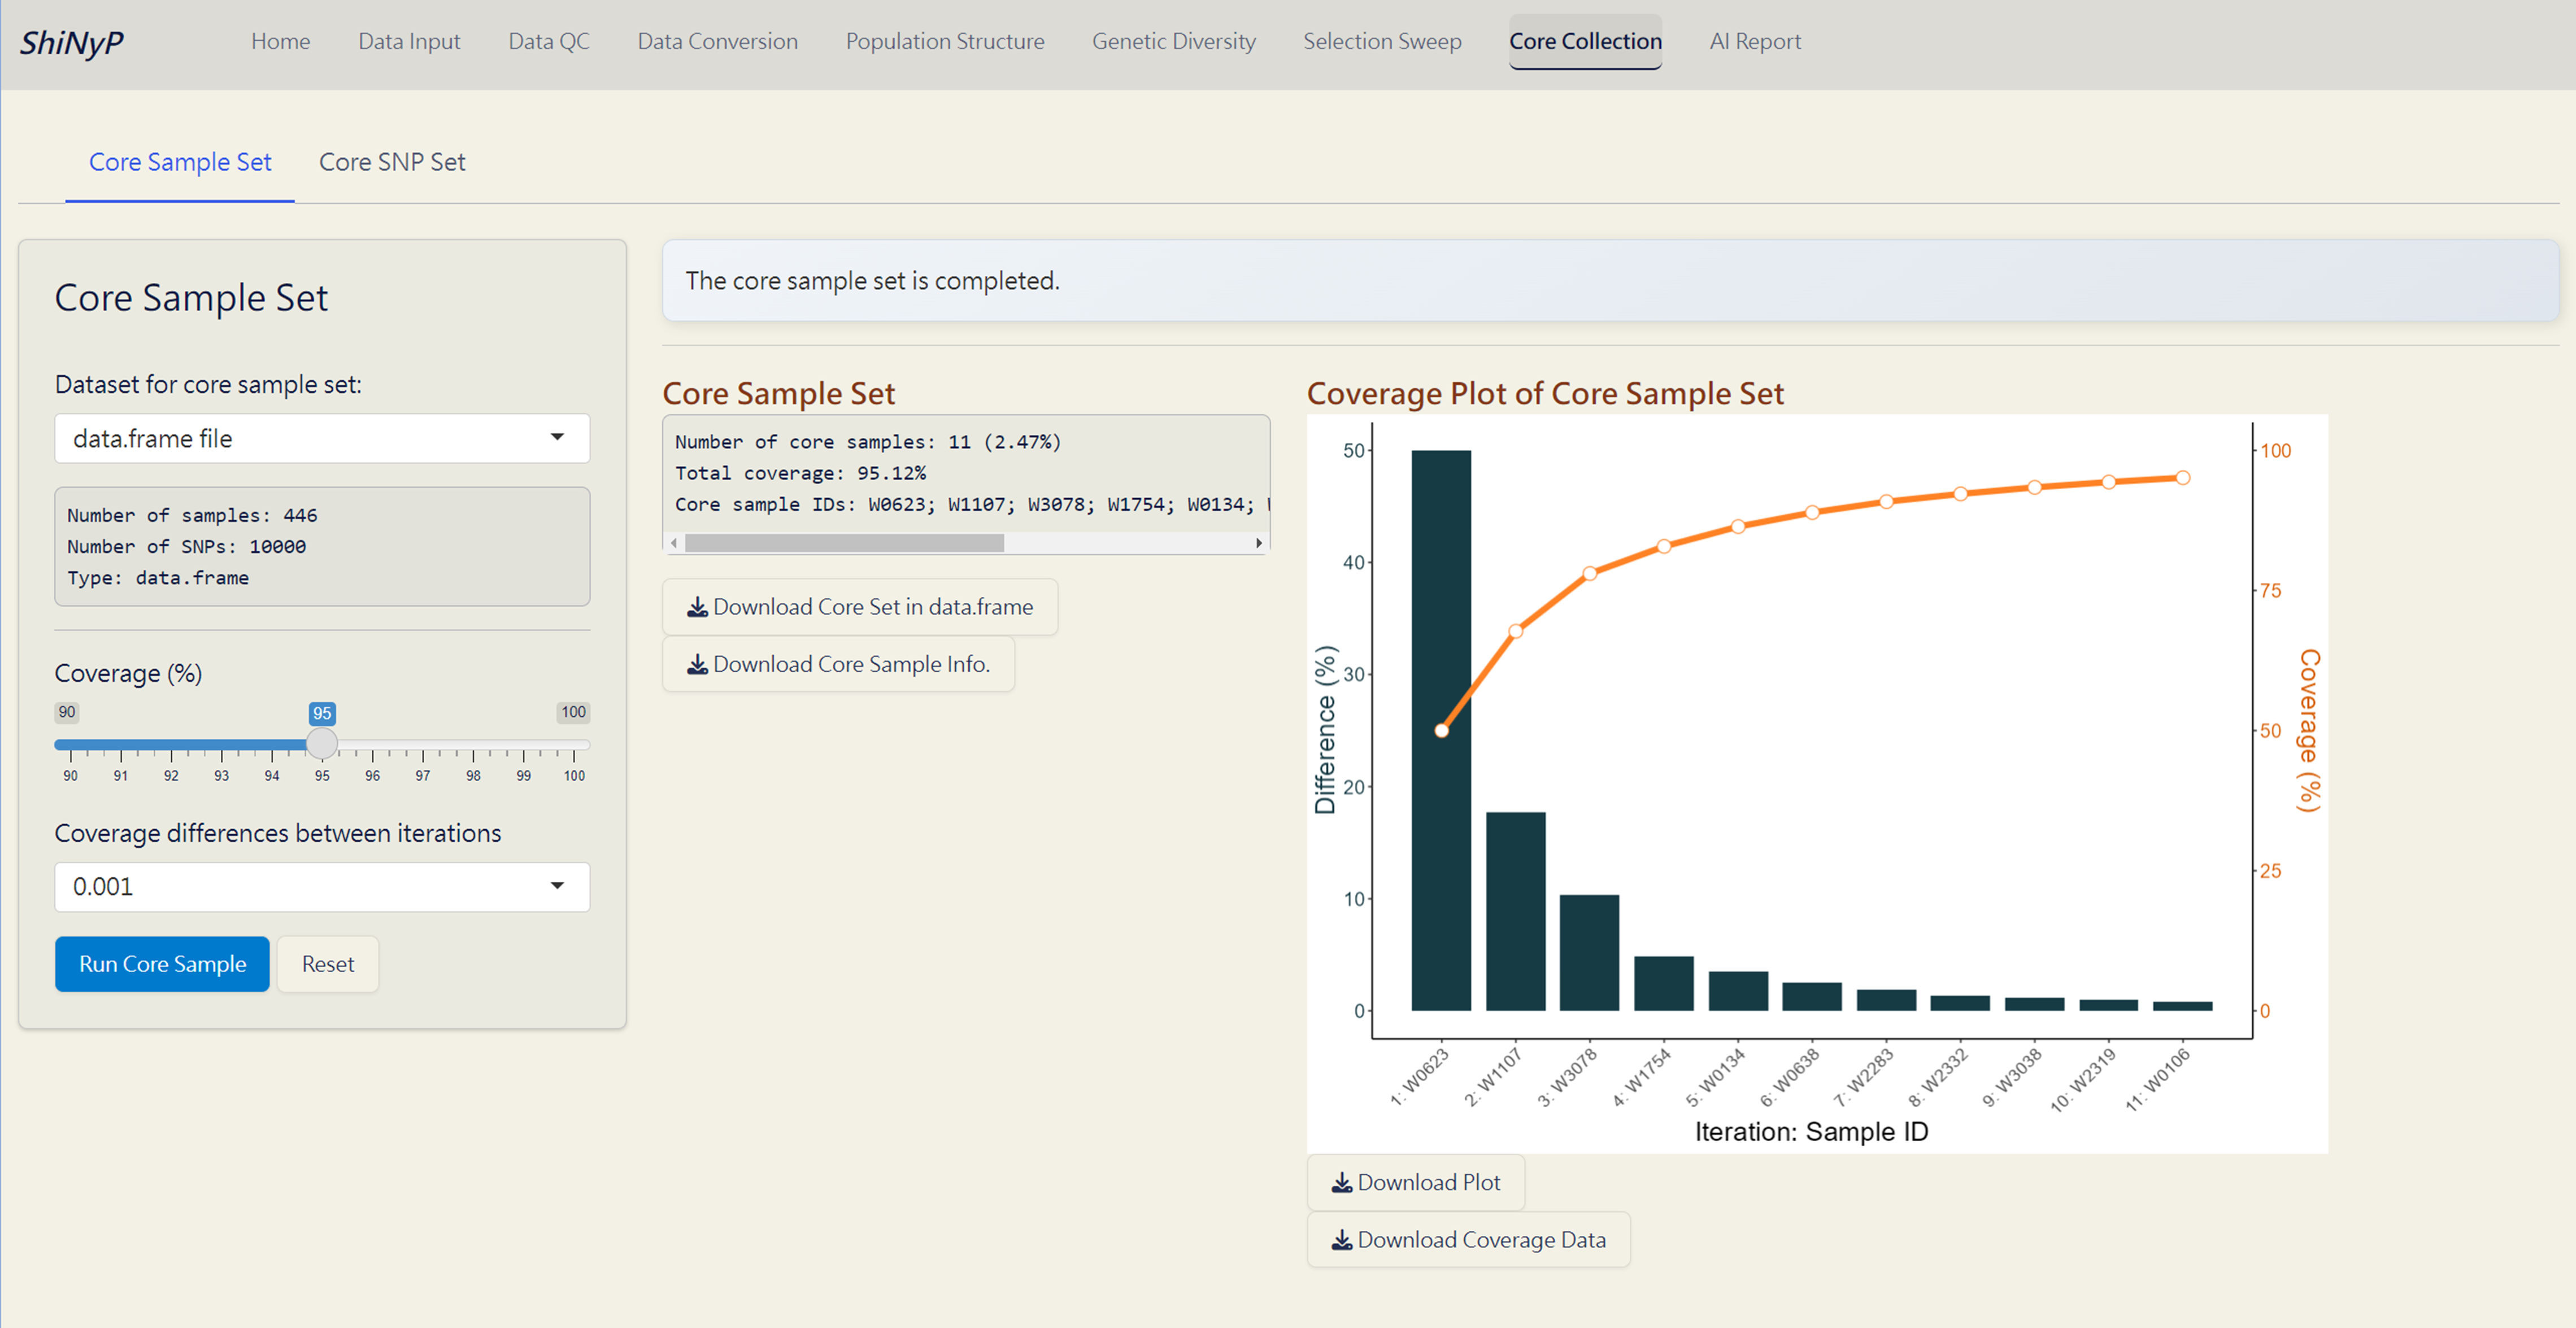
\includegraphics{images/clipboard-675369449.png}

\emph{The Core Sample Set Complete!}

\section{Core SNP Set}\label{core-snp-set}

Establish a core SNP collection that represents the genetic variation observed in the full dataset.

\paragraph*{Required Datasets:}\label{required-datasets-5}
\addcontentsline{toc}{paragraph}{Required Datasets:}

\begin{itemize}
\tightlist
\item
  {\textbf{\texttt{data.frame}}}
\item
  \textbf{Site Info.} \textbf{(RDS)} of the current {\textbf{\texttt{data.frame}}}, downloadable from \ul{Data Input} or \ul{Data QC} pages
\item
  \textbf{Chromosome Info.} \textbf{(CSV)}: Reference genome information of the current study. For more details about this file, refer to \textbf{Section} \ref{snp-density} \textbf{(SNP Density)}.
\item
  \textbf{DAPC Object} (DAPC\_dapc\_Object.rds), downloadable from \ul{Population Structure}/\ul{DAPC}.
\end{itemize}

\paragraph*{\texorpdfstring{\textbf{Steps:}}{Steps:}}\label{steps-12}
\addcontentsline{toc}{paragraph}{\textbf{Steps:}}

\begin{enumerate}
\def\labelenumi{\arabic{enumi}.}
\item
  {Upload} required datasts: \textbf{Site Info. (RDS)}, \textbf{Chromosome Info.} \textbf{(CSV)}, and \textbf{DAPC Object (RDS)}.
\item
  Choose the maximum core SNPs ratio (\%).
\item
  Click the {\textbf{Run Core SNP}} button to perform core collection.
\end{enumerate}

\paragraph*{Outputs:}\label{outputs-21}
\addcontentsline{toc}{paragraph}{Outputs:}

\begin{itemize}
\item
  \textbf{Core SNP Set (RDS)}: A {\textbf{\texttt{data.frame}}} of core SNPs and their genotypic information.
\item
  \textbf{Core SNP Info. (RDS)}: A table listing whether each SNP is included in the core collection or not.
\item
  \textbf{Distribution of Core SNPs (PDF)}: An ideogram labeling the core SNPs.
\item
  \textbf{Site Info. of Core SNPs (RDS)}: Core SNPs site information file.
\end{itemize}

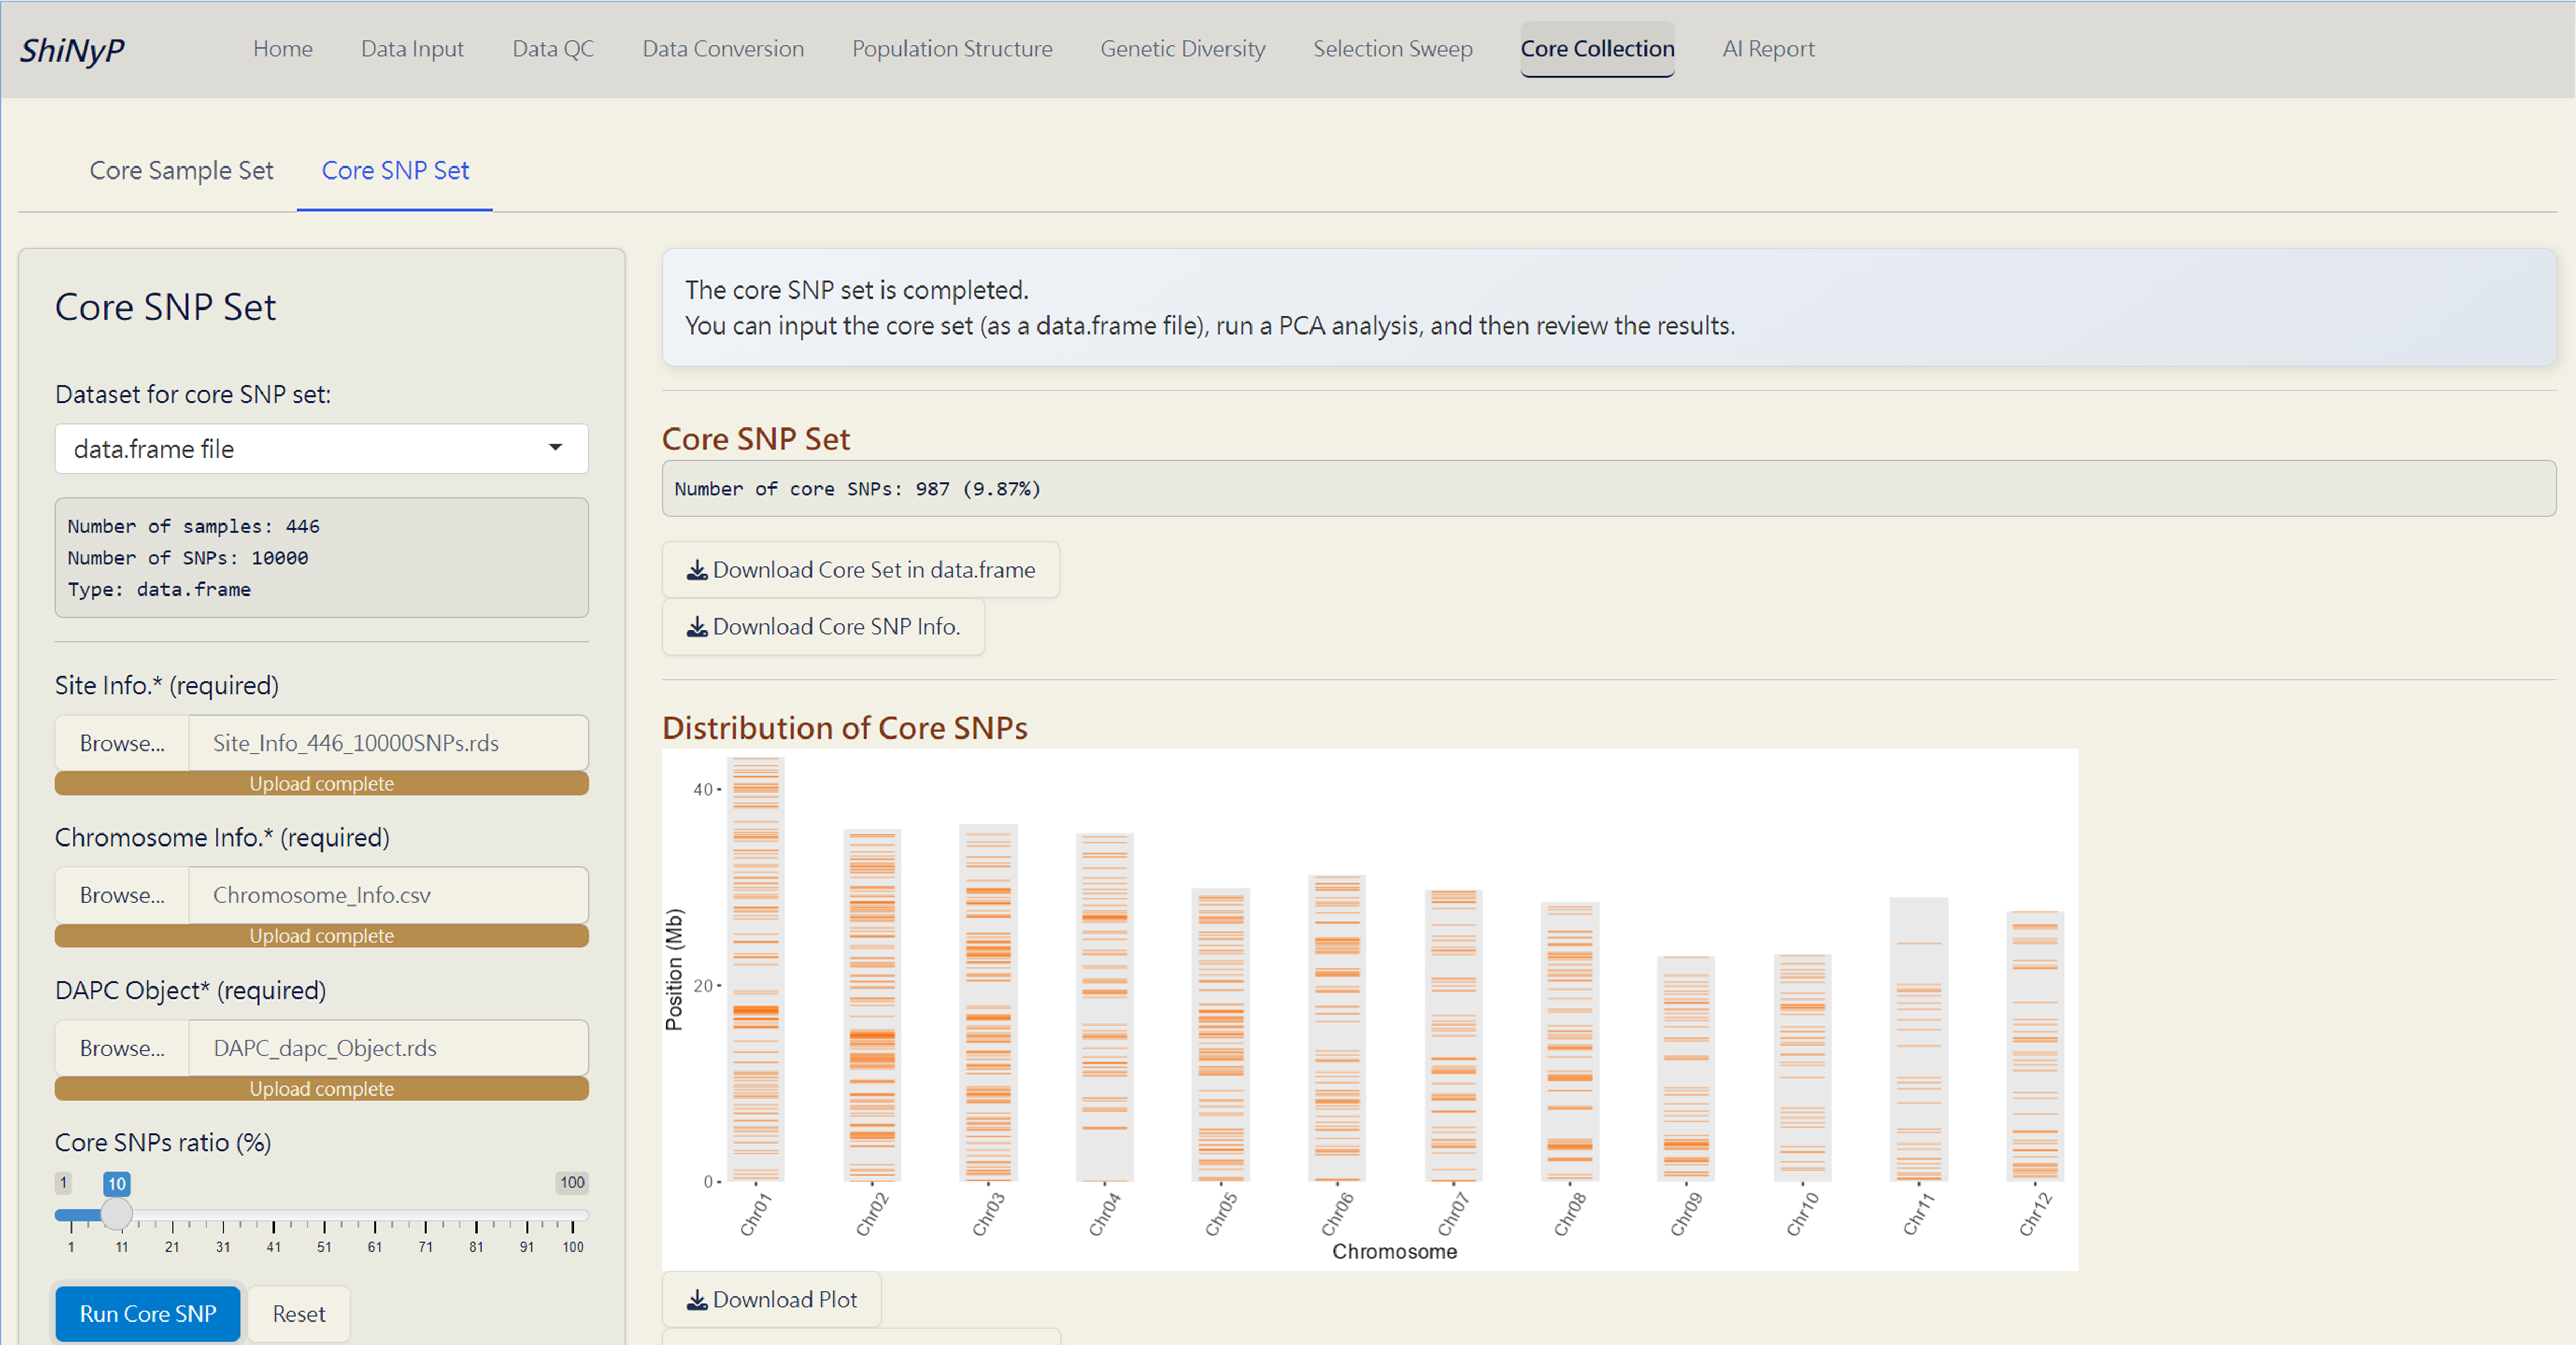
\includegraphics{images/clipboard-1144175211.png}

\emph{The Core SNP Set Complete!}

\chapter{AI Report}\label{sec-ai-report}

➡️ This page allows you to generate your preliminary results from prior analysis, input your OpenAI API key, select an AI model, and get an AI-driven report. Powered by the \emph{openai} package https://github.com/irudnyts/openai.

\paragraph*{Step 1: Preliminary Results}\label{step-1-preliminary-results}
\addcontentsline{toc}{paragraph}{Step 1: Preliminary Results}

\begin{enumerate}
\def\labelenumi{\arabic{enumi}.}
\item
  Enter the species name for the current study.
\item
  Click the {\textbf{Auto-generate}} button to obtain \textbf{Preliminary Results} from the {\textbf{\emph{ShiNyP}}} workflow.
\end{enumerate}

\begin{quote}
\textbf{Note}: You can download the Preliminary Results as a \texttt{.txt} file, edit it as needed, and upload it again for `AI-driven Report' use.
\end{quote}

\paragraph*{Step 2: AI-driven Report}\label{step-2-ai-driven-report}
\addcontentsline{toc}{paragraph}{Step 2: AI-driven Report}

\begin{enumerate}
\def\labelenumi{\arabic{enumi}.}
\item
  Select an AI model. We recommend using \textbf{GPT-4o mini}, which offers the most cost-efficient performance. For more information, see below \ref{how-to-get-the-openai-api-key} and visit: https://platform.openai.com/docs/models.
\item
  Specify the task for your Preliminary Results to OpenAI models (see below \ref{tasks-for-ai-models}).
\item
  Upload the \texttt{.txt} file containing your OpenAI API key (e.g., ``sk-\ldots\ldots{}'').

  ▼ Example of API key file (TXT).

  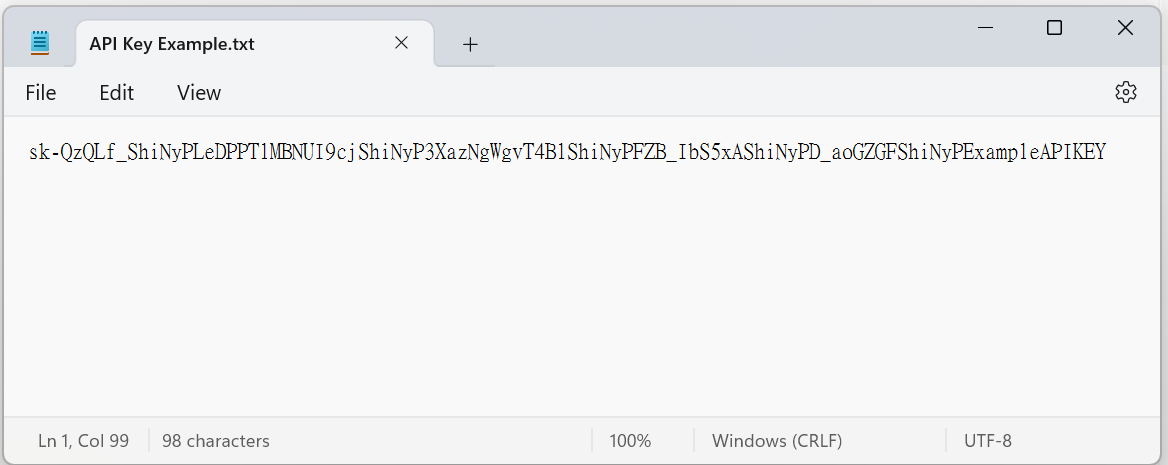
\includegraphics[width=4.6875in,height=\textheight]{images/clipboard-3104956900.png}
\item
  Click the {\textbf{Get Report}} button to obtain \textbf{AI-driven Report}.
\end{enumerate}

\begin{center}\rule{0.5\linewidth}{0.5pt}\end{center}

\paragraph*{Tasks for AI models:}\label{tasks-for-ai-models}
\addcontentsline{toc}{paragraph}{Tasks for AI models:}

\begin{itemize}
\item
  \textbf{Summary Request}: Generate a \ul{succinct overview of the key findings} from a genome-wide SNP analysis, ensuring clarity and a structured presentation of results.
\item
  \textbf{Data Interpretation}: Facilitate the analysis of genome-wide SNP data by \ul{elucidating findings and offering insights} into population structure and genetic variation.
\item
  \textbf{Report Structuring}: Develop a comprehensive framework for organizing and presenting the results of genome-wide SNP analysis in a \ul{scientific report} format.
\item
  \textbf{Idea Expansion}: Assist in brainstorming potential \ul{future research directions or experiments informed} by the results of the SNP analysis.
\end{itemize}

\begin{center}\rule{0.5\linewidth}{0.5pt}\end{center}

\paragraph*{\texorpdfstring{\textbf{How to get the OpenAI API key}:}{How to get the OpenAI API key:}}\label{how-to-get-the-openai-api-key}
\addcontentsline{toc}{paragraph}{\textbf{How to get the OpenAI API key}:}

\begin{enumerate}
\def\labelenumi{\arabic{enumi}.}
\item
  \textbf{Sign Up or Log In} to the OpenAI website: \url{https://platform.openai.com/docs/overview}.
\item
  \textbf{Check Your Usage} to track (free) credits and current consumption: \url{https://platform.openai.com/usage}.
\item
  If your (free) credits are \textbf{insufficient}, you can manage billing and payments by visiting: \url{https://platform.openai.com/settings/organization/billing/overview}.
\item
  \textbf{Generate a New API Key} by going to: \url{https://platform.openai.com/api-keys}.
\item
  \textbf{Copy and Paste} the generated key into a Notepad file and save it as a \texttt{.txt} file for {\textbf{\emph{ShiNyP}}} use.
\end{enumerate}

Upon signing up, OpenAI provides free credits valid for 3 months. After the free trial credits expire or are exhausted, you'll be billed based on your usage. Costs depend on the model and the number of tokens processed.

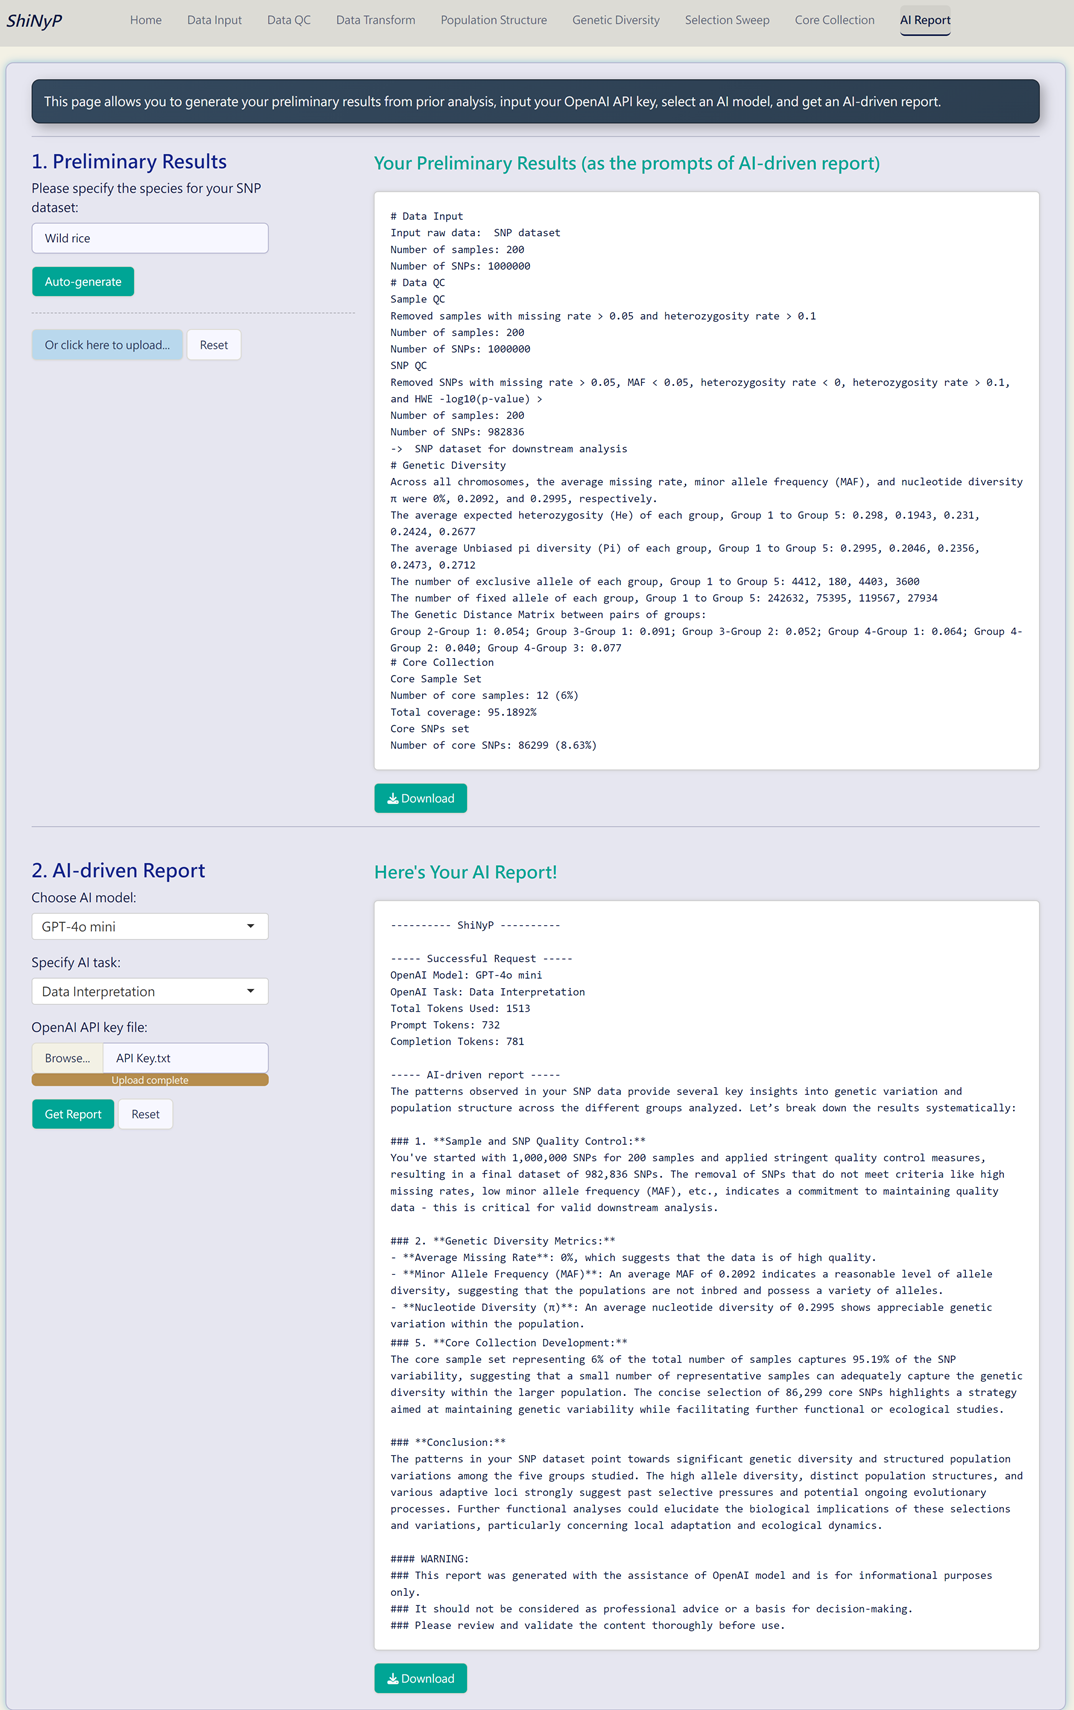
\includegraphics{images/clipboard-420815584.png}

\emph{The AI Report Complete!}

\begin{center}\rule{0.5\linewidth}{0.5pt}\end{center}

\paragraph*{Encountered an error? Let's fix it!}\label{encountered-an-error-lets-fix-it}
\addcontentsline{toc}{paragraph}{Encountered an error? Let's fix it!}

\begin{description}
\item[Error: HTTP 401 Unauthorized]
This error message indicates that your authentication credentials are invalid. This could happen for several reasons, such as:

\begin{itemize}
\item
  You are using a revoked API key.
\item
  You are using a different API key than one under the requesting organization.
\item
  You are using an API key that does not have the required permissions for the endpoint you are calling.
\end{itemize}

To resolve this error, first check that you are using the correct API key and organization ID in your request header. You can find your API key and organization ID in your account settings \href{https://platform.openai.com/account/api-keys}{here}.
\item[Error: Failed to Perform HTTP Request]
This error may indicate that the request timed out, possibly due to an excessive input token count, which prevents the OpenAI model from completing the task within the allotted time.

To resolve this issue, try selecting the `GPT-3.5 Turbo' model to generate the report first. If successful, you can then switch to other models for subsequent tasks.
\end{description}

\chapter{INDEX}\label{sec-index}

\begin{itemize}
\item
  AI Report \href{https://teddyenn.github.io/ShiNyP-guide/sec-ai-report.html\#sec-ai-report}{10}
\item
  AMOVA (Analysis of MOlecular VAriance) \href{https://teddyenn.github.io/ShiNyP-guide/sec-genetic-diversity.html\#amova-analysis-of-molecular-variance}{7.4}
\item
  API key \href{https://teddyenn.github.io/ShiNyP-guide/sec-ai-report.html\#step-2-ai-driven-report}{10}
\item
  Bayesian Information Criterion (BIC) \href{https://teddyenn.github.io/ShiNyP-guide/sec-population-structure.html\#step-2-dapc-analysis}{6.2}
\item
  Chromosome Info. \href{https://teddyenn.github.io/ShiNyP-guide/sec-data-qc.html\#snp-density}{4.3} \href{https://teddyenn.github.io/ShiNyP-guide/sec-genetic-diversity.html\#circos-plot}{7.2} \href{https://teddyenn.github.io/ShiNyP-guide/sec-selection-sweep.html\#ibs-identity-by-state}{8.3} \href{https://teddyenn.github.io/ShiNyP-guide/sec-selection-sweep.html\#manhattan-plot-plus}{8.4} \href{https://teddyenn.github.io/ShiNyP-guide/sec-core-collection.html\#core-snp-set}{9.2}
\item
  Circos Plot \href{https://teddyenn.github.io/ShiNyP-guide/sec-genetic-diversity.html\#circos-plot}{7.2}
\item
  Core Sample Set \href{https://teddyenn.github.io/ShiNyP-guide/sec-core-collection.html\#core-sample-set}{9.1}
\item
  Core SNP Set \href{https://teddyenn.github.io/ShiNyP-guide/sec-core-collection.html\#core-snp-set}{9.2}
\item
  DAPC (Discriminant Analysis of Principal Components) \href{https://teddyenn.github.io/ShiNyP-guide/sec-population-structure.html\#dapc-discriminant-analysis-of-principal-components}{6.2}
\item
  data.frame \href{https://teddyenn.github.io/ShiNyP-guide/sec-data-input.html\#step-2-transform-to-data.frame}{3.1}
\item
  Demo Data \href{https://teddyenn.github.io/ShiNyP-guide/sec-data-input.html\#step-1-input-your-vcf-file}{3.1}
\item
  Diversity Parameter \href{https://teddyenn.github.io/ShiNyP-guide/sec-genetic-diversity.html\#diversity-parameter}{7.1}
\item
  Genetic Distance \href{https://teddyenn.github.io/ShiNyP-guide/sec-genetic-diversity.html\#genetic-distance}{7.3}
\item
  genind \href{https://teddyenn.github.io/ShiNyP-guide/sec-data-conversion.html\#step-1-transform-data.frame-to-genind}{5}
\item
  genlight \href{https://teddyenn.github.io/ShiNyP-guide/sec-data-conversion.html\#step-2-transform-genind-to-genlight}{5}
\item
  Group Info. \href{https://teddyenn.github.io/ShiNyP-guide/sec-data-conversion.html\#step-1-transform-data.frame-to-genind}{5} \href{https://teddyenn.github.io/ShiNyP-guide/sec-population-structure.html\#kinship-analysis}{6.5} \href{https://teddyenn.github.io/ShiNyP-guide/sec-population-structure.html\#scatter-plot-plus}{6.6} \href{https://teddyenn.github.io/ShiNyP-guide/sec-genetic-diversity.html\#diversity-parameter}{7.1} \href{https://teddyenn.github.io/ShiNyP-guide/sec-selection-sweep.html\#outflank}{8.2}
\item
  Hardy-Weinberg equilibrium (HWE) \href{https://teddyenn.github.io/ShiNyP-guide/sec-data-qc.html\#snp-qc}{4.2}
\item
  Heterozygosity rate \href{https://teddyenn.github.io/ShiNyP-guide/sec-data-qc.html\#sample-qc}{4.1}
\item
  IBS (Identity By State) \href{https://teddyenn.github.io/ShiNyP-guide/sec-selection-sweep.html\#ibs-identity-by-state}{8.3}
\item
  Kinship Analysis \href{https://teddyenn.github.io/ShiNyP-guide/sec-population-structure.html\#kinship-analysis}{6.5}
\item
  Manhattan Plot \href{https://teddyenn.github.io/ShiNyP-guide/sec-selection-sweep.html\#manhattan-plot-plus}{8.4}
\item
  Minor allele frequency (MAF) \href{https://teddyenn.github.io/ShiNyP-guide/sec-data-qc.html\#snp-qc}{4.2}
\item
  Missing rate \href{https://teddyenn.github.io/ShiNyP-guide/sec-data-qc.html\#sample-qc}{4.1}
\item
  NJ (Neighbor-Joining) Tree \href{https://teddyenn.github.io/ShiNyP-guide/sec-population-structure.html\#nj-neighbor-joining-tree}{6.4}
\item
  OutFLANK \href{https://teddyenn.github.io/ShiNyP-guide/sec-selection-sweep.html\#outflank}{8.2}
\item
  PCA (Principal Component Analysis) \href{https://teddyenn.github.io/ShiNyP-guide/sec-population-structure.html\#pca-principal-component-analysis}{6.1}
\item
  pcadapt \href{https://teddyenn.github.io/ShiNyP-guide/sec-selection-sweep.html\#pcadapt}{8.1}
\item
  Permutation Test \href{https://teddyenn.github.io/ShiNyP-guide/sec-genetic-diversity.html\#step-2-run-permutation-test}{7.4}
\item
  Sample QC \href{https://teddyenn.github.io/ShiNyP-guide/sec-data-qc.html\#sample-qc}{4.1}
\item
  Scatter Plot \href{https://teddyenn.github.io/ShiNyP-guide/sec-data-qc.html\#sample-qc}{6.6}
\item
  \emph{ShiNyP} \href{https://teddyenn.github.io/ShiNyP-guide/sec-shinyp.html\#sec-shinyp}{2}
\item
  Site Info. \href{https://teddyenn.github.io/ShiNyP-guide/sec-data-input.html\#step-2-transform-to-data.frame}{3.1} \href{https://teddyenn.github.io/ShiNyP-guide/sec-data-qc.html\#sample-qc}{4.1} \href{https://teddyenn.github.io/ShiNyP-guide/sec-data-qc.html\#snp-qc}{4.2} \href{https://teddyenn.github.io/ShiNyP-guide/sec-data-qc.html\#snp-density}{4.3} \href{https://teddyenn.github.io/ShiNyP-guide/sec-genetic-diversity.html\#diversity-parameter}{7.1} \href{https://teddyenn.github.io/ShiNyP-guide/sec-selection-sweep.html\#pcadapt}{8.1} \href{https://teddyenn.github.io/ShiNyP-guide/sec-selection-sweep.html\#outflank}{8.2} \href{https://teddyenn.github.io/ShiNyP-guide/sec-selection-sweep.html\#ibs-identity-by-state}{8.3} \href{https://teddyenn.github.io/ShiNyP-guide/sec-core-collection.html\#core-snp-set}{9.2}
\item
  SNP Density \href{https://teddyenn.github.io/ShiNyP-guide/sec-data-qc.html\#snp-density}{4.3}
\item
  SNP QC \href{https://teddyenn.github.io/ShiNyP-guide/sec-data-qc.html\#snp-qc}{4.2}
\item
  Tree Plot \href{https://teddyenn.github.io/ShiNyP-guide/sec-population-structure.html\#tree-plot-plus}{6.7}
\item
  UPGMA (Unweighted Pair Group Method with Arithmetic mean) Tree \href{https://teddyenn.github.io/ShiNyP-guide/sec-population-structure.html\#upgma-unweighted-pair-group-method-with-arithmetic-mean-tree}{6.3}
\item
  VCF \href{https://teddyenn.github.io/ShiNyP-guide/sec-data-input.html\#vcf}{3.1}
\end{itemize}

\begin{center}\rule{0.5\linewidth}{0.5pt}\end{center}

\subsubsection*{Bibliography}\label{bibliography}
\addcontentsline{toc}{subsubsection}{Bibliography}

  \bibliography{book.bib,packages.bib}

\end{document}
